\documentclass[twoside]{nsm-thesis}
% options:
% [germanthesis] - Thesis is written in German
% [plainunnumbered] - Don't print numbers on plain pages
% [earlydraft] - Settings for quick draft printouts
% [watermark] - Print current time/date at bottom of each page
% [phdthesis] - switch to PhD thesis style
% [twoside] - double-sided
% [cutmargins] - text body fills complete page

% 1. Load Configuration and Metadata
% Add specific packages here if needed later
% \usepackage{listings}
% LaTeX TikZ Code
\usepackage{tikz}
\usetikzlibrary{matrix, positioning, arrows.meta, fit, backgrounds, calc}
% Scale wide tables down to fit textwidth (scales only when content exceeds \linewidth)
\usepackage{adjustbox}
% Author name; separate multiple authors with commas.
\author{Abdulaziz Musaev}
\birthday{22nd November, 1999}
\birthplace{Denau, Uzbekistan}

\title{A Comparative Analysis of WebAssembly and Docker Containers for Microservice Architectures in Kubernetes}

% Choose one of the following lines.
% \thesistype{Seminar Thesis}
%\thesistype{Bachelor Thesis}
\thesistype{Master's Thesis}
%\thesistype{Diploma Thesis}

% Choose one of the following lines or amend as necessary.
%\degreeprogram{Computer Science}
%\degreeprogram{Computational Logic}
%\degreeprogram{Computational Modeling and Simulation}
\degreeprogram{Distributed Systems Engineering}
%\degreeprogram{Information Systems Engineering}
%\degreeprogram{Media Informatics}

% List of advisors, separated by commas; comment out if not needed.
\advisors{Dr. Michael Steininger}

% List of referees, separated by commas.
\referees{Prof. Dr. Christof Fetzer, Dr. K. Pubudu N. Jayasena}
% Define abbreviations used in the thesis here.
\acrodef{WSN}{Wireless Sensor Network}
\acrodef{MANET}{Mobile Ad Hoc Network}
\acrodef{ROI}{Region of Interest}{short-indefinite={an}, long-plural-form={Regions of Interest}}
\acrodef{ADAC}{German Automobile Association}{foreign={Allgemeiner Deutscher Automobilclub}}
\acrodef{CANhashing}[CAN]{Content Addressable Network}{extra={when referring to the distributed hash table}}
\acrodef{CANproto}[CAN]{Controller Area Network}{extra={when referring to the bus protocol}}

\begin{document}

% 2. Frontmatter (Roman numbering)
\pagenumbering{roman}
\maketitle
\cleardoublepage

% Abstract
\chapter*{Abstract}
\addcontentsline{toc}{chapter}{Abstract}
\begin{otherlanguage*}{american}

about 1/2 page:
\begin{enumerate}
    \item Motivation (Why do we care?)
    \item Problem statement (What problem are we trying to solve?)
    \item Approach (How did we go about it)
    \item Results (What's the answer?)
    \item Conclusion (What are the implications of the answer?)
\end{enumerate}

The abstract is a miniature version of the thesis.
It should be treated as an entirely separate document.
Do not assume that a reader who has access to an abstract will also have access to the thesis.
Do not assume that a reader who reads the thesis has read the abstract.

\end{otherlanguage*}

% Table of Contents
\cleardoublepage
\tableofcontents
\cleardoublepage

% 3. Main Content (Arabic numbering)
\pagenumbering{arabic}

\chapter{Introduction}
\label{chap:introduction}

\section{Context}
The modern cloud computing landscape relies heavily on microservices and containerization to deliver scalable, resilient applications. Docker and the Open Container Initiative (OCI) standards, frequently paired with mature backend languages like Golang, have become the de facto foundation for these deployments within Kubernetes environments \cite{merkel2014docker, burns2016borg}. This traditional cloud-native stack prioritizes a frictionless developer experience and mature tooling. However, the growing demand for edge computing, high-density serverless functions, and instantaneous scaling has exposed the architectural limitations of conventional Linux containers. OCI containers rely on operating-system-level virtualization, which carries a baseline overhead in both memory consumption and initialization time \cite{shillaker2020faasm}.

As organizations seek to maximize hardware utilization and minimize latency, a shift toward more lightweight execution environments is underway. WebAssembly (Wasm), originally designed as a highly optimized, stack-based virtual machine binary format for web browsers \cite{haas2017bringing}, has emerged as a potential solution for server-side workloads. With the introduction of the WebAssembly System Interface (WASI), Wasm promises a portable, secure, and near-instantaneous execution model that operates without the heavy dependencies of a traditional Linux container \cite{lin2022wasmedge}.

\section{Problem Statement}
Standard OCI containers introduce measurable overhead regarding memory footprint and cold-start latency. While negligible for traditional monolithic applications, this overhead becomes a severe limiting factor for transient microservices that require rapid, sub-millisecond scaling. The emerging WebAssembly stack theoretically solves this by utilizing software-based fault isolation (SFI) to strip away the operating system layer entirely, offering drastically reduced image sizes and high-density execution \cite{gadepalli2020challenges}.

However, transitioning from a mature ecosystem to a nascent one introduces substantial, often under-documented friction. The core problem this thesis addresses is the tension between computational efficiency and developer velocity. While the Wasm ecosystem promises high performance for server-side workloads, it currently lacks robust multithreading capabilities, enforces strict limitations on compiled network dependencies, and demands specialized expertise in systems languages like Rust. 

There is a critical need to empirically quantify the holistic trade-offs of these two paradigms. It must be determined whether the theoretical efficiency gains of the Wasm stack outweigh the practical performance degradations and the operational complexities it introduces compared to the industry-standard Docker baseline.

\section{Research Questions}
To address the problem statement, this thesis investigates the following primary research questions:
\begin{itemize}
    \item \textbf{RQ1:} How does the memory footprint and image size of the emerging Wasm stack compare to a traditional Docker baseline in a Kubernetes environment?
    \item \textbf{RQ2:} To what extent do WebAssembly runtimes improve cold and warm startup latencies compared to standard OCI container runtimes executing garbage-collected binaries?
    \item \textbf{RQ3:} What are the runtime performance trade-offs—specifically regarding request throughput and execution latency—introduced by WebAssembly’s current constraints on multithreading compared to Golang's native concurrency model?
    \item \textbf{RQ4:} How do ecosystem limitations, specifically regarding the Rust learning curve, WASI compatibility, and CI/CD integration, impact the developer experience and maintainability when migrating from a traditional containerized pipeline?
\end{itemize}

\section{Research Methodology}
This research employs a mixed-methods approach, combining quantitative performance benchmarking with a qualitative assessment of developer experience. 

Rather than isolating the runtime—which would necessitate comparing equivalent languages and thereby destroying the ability to measure real-world developer experience—this study compares the two dominant paradigms in their native contexts. First, a baseline microservice is developed using Golang and compiled into a standard Linux-based Docker image. Second, a functionally equivalent alternative is developed using Rust and compiled into a WASI-compliant WebAssembly module. Both artifacts are deployed into an isolated Kubernetes test cluster utilizing \texttt{containerd}, standard \texttt{runc}, and a Wasm shim. 

Quantitative data is gathered by subjecting both deployments to standardized load testing. Monitoring tools are used to measure cold-start times, memory consumption, CPU utilization, throughput, and request latency. While this approach acknowledges that language-level differences (e.g., Go's garbage collection versus Rust's manual memory management) influence the final metrics, it is strictly designed to reflect the real-world performance delta an engineering team experiences when transitioning between these technological stacks. Second, a qualitative analysis is conducted on the development lifecycle, documenting compilation friction, library compatibility, and pipeline integration complexity.

\section{Thesis Contributions}
This thesis provides the following key contributions to the field of cloud-native architecture:
\begin{enumerate}
    \item \textbf{Holistic Paradigm Benchmark:} A side-by-side performance comparison of the Golang/Docker stack versus the Rust/Wasm stack, highlighting specific metrics where the Wasm ecosystem succeeds (density, initialization) and where it currently fails (throughput, computational latency).
    \item \textbf{Developer Experience Assessment:} A critical evaluation of the current state of WebAssembly for backend development, quantifying the engineering friction of compiling Rust code to WASI and navigating incompatible library dependencies compared to standard Go development.
    \item \textbf{Adoption Framework:} Actionable recommendations for cloud architects, delineating specific use cases where the Rust/Wasm stack is currently viable and identifying the operational risks that make it unsuitable for rapid-iteration product teams accustomed to the Go/Docker ecosystem.
\end{enumerate}

\section{Thesis Structure}
The remainder of this thesis is structured as follows:
\begin{itemize}
    \item \textbf{Chapter 2: Background} provides the foundational technical context on cloud computing paradigms, containerization technologies, the Go concurrency model, and the evolution of WebAssembly and WASI.
    \item \textbf{Chapter 3: State of the Art} reviews the theoretical foundations of Wasm's security, the emerging Component Model, and current industry adoption.
    \item \textbf{Chapter 4: Research Methodology} defines the comparative analysis strategy, establishing the Golang/Docker baseline against the Rust/Wasm challenger, and outlines the precise metrics.
    \item \textbf{Chapter 5: Implementation} details the system architecture, service design, compilation processes, and Kubernetes cluster configuration for both environments.
    \item \textbf{Chapter 6: Evaluation} presents the quantitative benchmark results alongside the qualitative assessment of the developer experience.
    \item \textbf{Chapter 7: Discussion and Future Work} analyzes the trade-offs between technological maturity, computational efficiency, and developer velocity.
    \item \textbf{Chapter 8: Conclusion} summarizes the core findings and final verdicts of the research.
\end{itemize}
\chapter{Background}
\label{chap:background}

This chapter provides the foundational technical context required to evaluate the comparative analysis presented in this thesis. It traces the evolution of computing infrastructure from on-premises hardware to modern cloud paradigms, details the mechanics of containerization and orchestration, and culminates in a comprehensive architectural breakdown of WebAssembly as an emerging server-side execution environment.

\section{Cloud Computing and Microservices}
\label{sec:cloud_microservices}

\subsection{The Evolution of Cloud Paradigms}
The genesis of modern software deployment traces back to on-premises data centers, where organizations were solely responsible for the procurement, maintenance, and scaling of physical hardware. This capital-heavy model suffered from severe resource underutilization; servers were provisioned for peak load, leaving them idle during standard operations. The modern cloud computing era shifted the industry to a pay-as-you-go, scalable operational model, fundamentally altering how infrastructure is managed ~\cite{mell2011nist}.

As cloud computing matured, the industry developed a "Shared Responsibility Model," where the abstraction layer moved progressively higher up the stack. This spectrum dictates whether the cloud provider or the client is responsible for specific layers of the technological stack:

\begin{itemize}
    \item \textbf{Infrastructure as a Service (IaaS):} The cloud provider manages the physical hardware, storage, and networking. The client rents virtualized infrastructure (e.g., a Virtual Machine) and retains full responsibility for managing the operating system, middleware, language runtimes, and the application code itself. This offers maximum control but requires significant operational overhead.
    \item \textbf{Platform as a Service (PaaS):} The provider abstracts both the underlying hardware and the operating system. The client is provided a managed environment and is solely responsible for deploying their application code and managing their data. Traditional Docker container deployments often operate in this space.
    \item \textbf{Function as a Service (FaaS) / Serverless:} The highest level of \textit{infrastructure} abstraction for a developer. The cloud provider dynamically manages the allocation, provisioning, and scaling of the servers and runtimes. The client writes granular, event-driven functions and dictates the trigger configurations. The client is still strictly responsible for the software architecture and code quality. Crucially, FaaS allows applications to "scale to zero," eliminating compute costs during periods of inactivity ~\cite{jonas2019cloud}.
    \item \textbf{Software as a Service (SaaS):} The highest level of \textit{software} abstraction. The cloud provider hosts and manages the entire application stack—from the hardware and OS up to the application code itself. The client manages nothing regarding the deployment or execution environment; they simply consume the finished software over the internet (e.g., Google Workspace, Salesforce).
\end{itemize}

\begin{figure}[htbp]
    \centering
    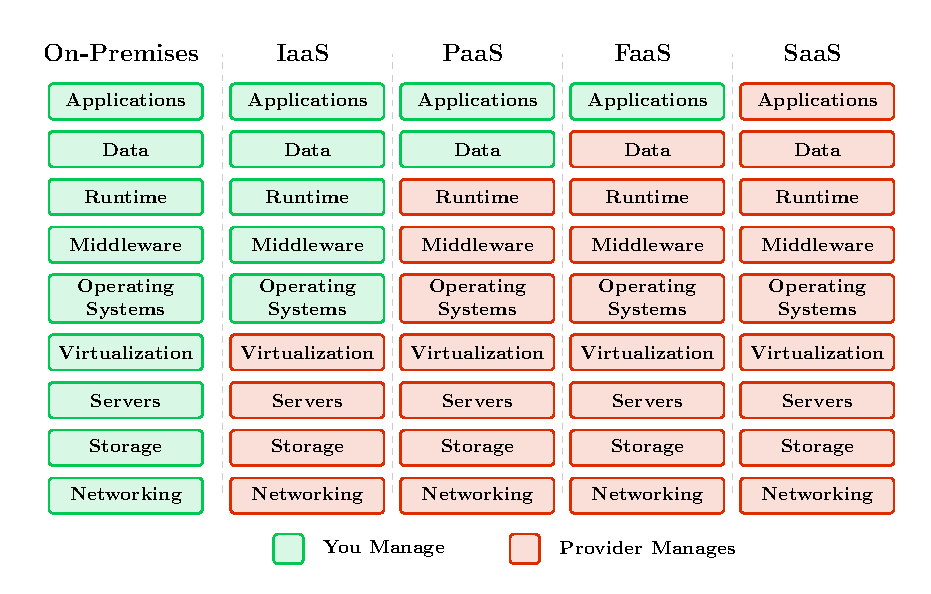
\includegraphics[width=0.8\textwidth]{figures/iaas_paas_faas_saas.pdf}
    \caption{The Shared Responsibility Model across varying Cloud Computing Paradigms.}
    \label{fig:iaas_paas_faas_saas}
\end{figure}

For the purposes of this research, SaaS falls outside the scope of architectural implementation. The critical transition lies between PaaS and FaaS. The relentless industry drive toward rapid elasticity, microsecond billing, and extreme resource efficiency in FaaS and edge environments exposed the limitations of traditional, heavy deployment artifacts. Developers pushing code to serverless platforms require instantaneous execution. Standard OCI containers, laden with operating system userlands, introduce severe latency bottlenecks in these paradigms, necessitating a shift toward the lightweight isolation models that WebAssembly provides.

\subsection{Microservice Architecture}
Microservice architecture emerged as the logical software design pattern for cloud-native deployment. Unlike traditional monolithic applications—where all business logic, user interfaces, and database connections are tightly coupled into a single executable—microservices decompose an application into a collection of small, independently deployable, and loosely coupled services that communicate over a network via language-agnostic APIs ~\cite{newman2015building}.

This paradigm offers distinct advantages: development agility, localized fault isolation, and the ability to scale specific system bottlenecks independently. However, it introduces severe distributed system challenges. Managing network latency, data consistency, and the operational overhead of packaging and deploying hundreds of individual services necessitated the creation of entirely new virtualization and orchestration layers.

\section{Containerization and Orchestration}
\label{sec:containerization}

\subsection{Virtual Machines vs. Containers}
To solve the deployment complexity of microservices, the industry initially relied on Virtual Machines. However, VMs require a hypervisor to emulate physical hardware, atop which a complete guest OS is installed. This results in gigabytes of memory overhead and startup times measured in minutes, making them inherently unsuitable for transient, rapidly scaling microservices.

Docker revolutionized the landscape by democratizing Linux containers. Instead of virtualizing the hardware, containers virtualize the operating system ~\cite{merkel2014docker}. Docker relies on two core Linux kernel features:
\begin{enumerate}
    \item \textbf{Namespaces:} Provide process isolation, ensuring the container has its own isolated filesystem, network interfaces, and process tree.
    \item \textbf{Cgroups (Control Groups):} Limit, isolate, and monitor the resource usage (CPU, memory, disk I/O) of a given process.
\end{enumerate}

\begin{figure}[htbp]
    \centering
    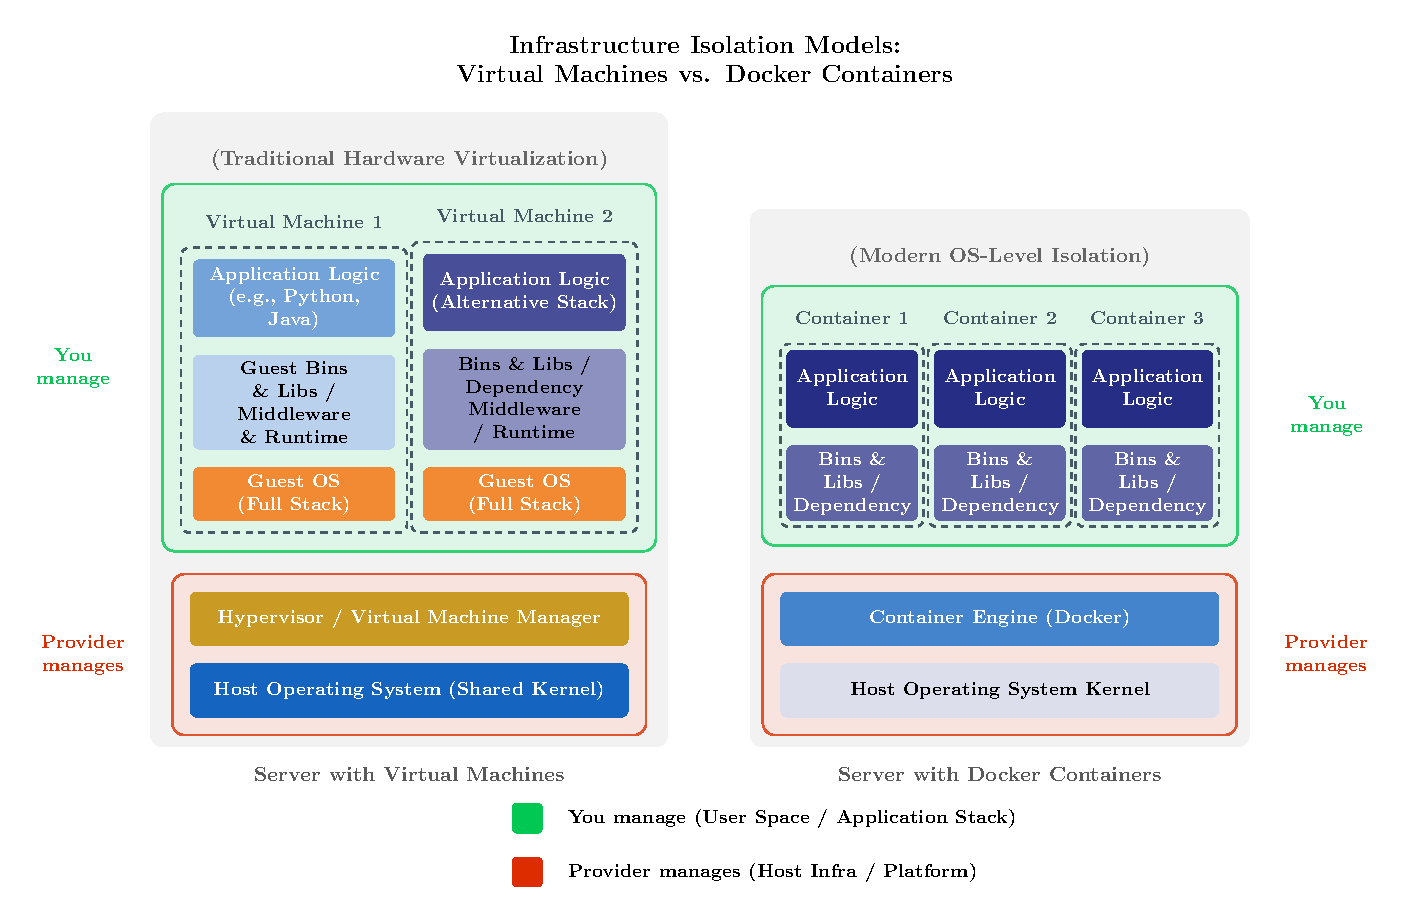
\includegraphics[width=\textwidth]{figures/virtual_machine_vs_docker.pdf}
    \caption{Infrastructure Isolation Models: Virtual Machines vs. Docker Containers}
    \label{fig:virtual_machine_vs_docker}
\end{figure}

Docker’s definitive innovation was the standardization of the container image format, now governed by the Open Container Initiative (OCI). By packaging application code alongside its dependencies, libraries, and a base filesystem into a single portable unit, Docker ensured environment consistency from a developer's laptop to production servers.

Despite its dominance, the OCI standard has inherent drawbacks. Because containers share the host's Linux kernel, a kernel-level vulnerability can potentially compromise all containers on that host, posing security risks in multi-tenant environments. Furthermore, traditional container images are bulky; they bundle a userland OS and language runtimes alongside the application. This bulk introduces latency during image transfer and initialization—known as the "cold start" problem—which is highly detrimental in FaaS and edge computing environments ~\cite{gadepalli2020challenges}.

\subsection{Kubernetes Orchestration}
As microservices proliferated, manually managing individual containers across a fleet of servers became operationally unfeasible. Kubernetes emerged as the industry-standard container orchestration platform. It abstracts the underlying cluster of hardware, allowing engineers to declare the desired state of their applications rather than manually scripting deployments ~\cite{burns2016borg}.

Kubernetes operates on a distributed architecture. The Control Plane dictates instructions to worker nodes. Each worker node runs an agent called a Kubelet, which manages Pods—the smallest deployable computing unit, typically containing one or more tightly coupled containers. Crucially, Kubernetes communicates with the underlying container runtime (like containerd or CRI-O) via the Container Runtime Interface (CRI). This decoupled architecture established strict standardizations, eventually allowing alternative, non-Linux execution environments, such as WebAssembly, to be orchestrated seamlessly alongside standard OCI-compliant containers.

\begin{figure}[htbp]
    \centering
    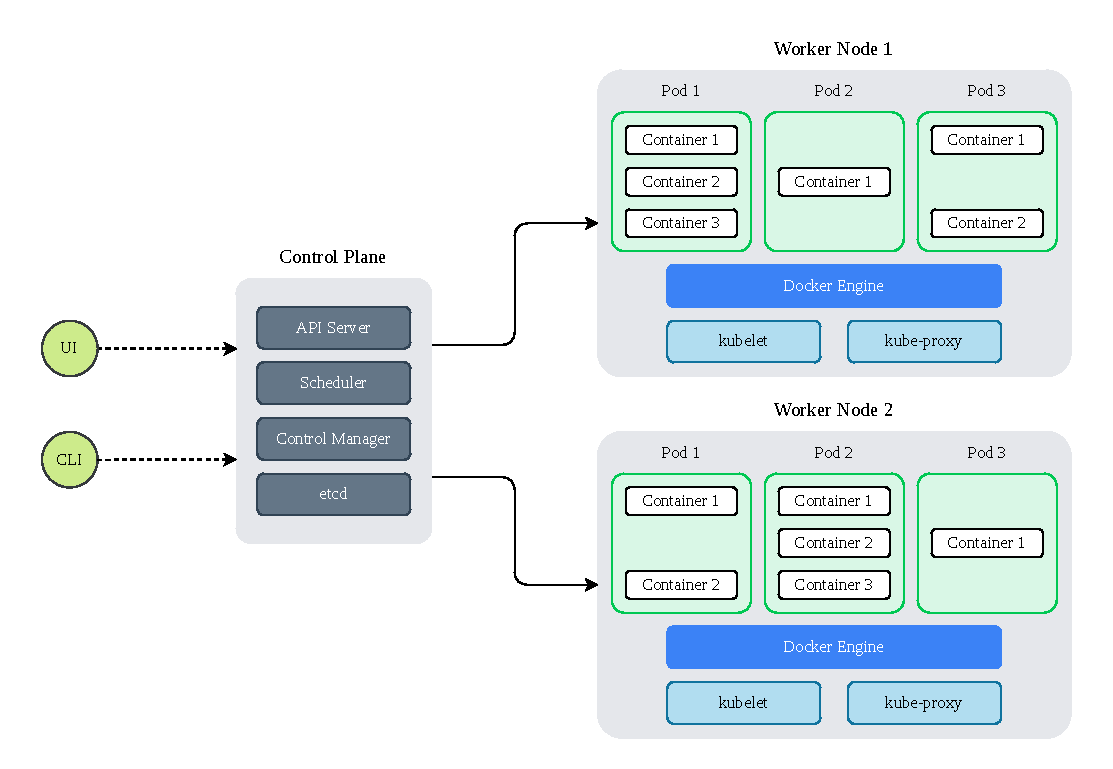
\includegraphics[width=0.8\textwidth]{figures/k8s_architecture.pdf}
    \caption{Kubernetes Architecture}
    \label{fig:kubernetes_architecture}
\end{figure}

\section{WebAssembly (Wasm)}
\label{sec:wasm}

\subsection{Origin and Technical Architecture}
WebAssembly (Wasm) is a binary instruction format designed for a stack-based virtual machine. It originated from the need to execute high-performance code within web browsers—a domain historically constrained by JavaScript's inconsistent performance and parsing overhead. WebAssembly was officially released in 2017 as a W3C standard, sitting alongside HTML, CSS, and JavaScript as an official language of the web ~\cite{haas2017bringing}.

Wasm functions as an agnostic hardware abstraction layer. Developers write code in systems languages like C, C++, or Rust, and compile it down to \texttt{.wasm} binaries. 

\begin{figure}[htbp]
    \centering
    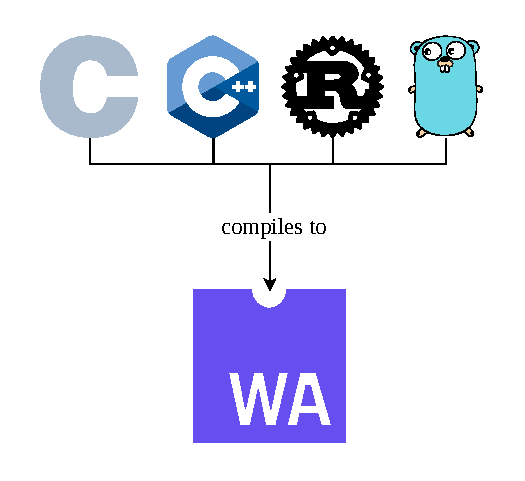
\includegraphics[width=0.5\textwidth]{figures/languages_compile_to_wasm.pdf}
    \caption{Compiling different languages to Wasm}
    \label{fig:compiling_different_langauges_to_wasm}
\end{figure}

\subsection{Module Structure and Stack-Based Execution}
WebAssembly is fundamentally a stack machine. Unlike register-based physical CPU architectures (such as x86\_64 or ARM64), Wasm instructions implicitly operate on an operand stack. Variables are pushed onto the stack, and operations pop these operands, compute the result, and push it back.  This design yields highly compact binary modules, as instructions do not need to explicitly encode register numbers, accelerating both transmission over networks and decoding phases.

A Wasm application is distributed as a strictly standardized binary module consisting of discrete sections. These include the Type section (function signatures), Import section (host-provided dependencies), Code section (executable bytecode), and Data section (initial memory state). Before execution, a WebAssembly runtime performs a deterministic, single-pass validation to ensure type safety and structural integrity. Because the bytecode is designed to map cleanly to native machine instructions, runtimes employ Just-In-Time (JIT) or Ahead-Of-Time (AOT) compilation engines (such as Cranelift or LLVM) to translate Wasm into highly optimized, native machine code instantaneously.

\subsection{Memory Management and Isolation}
One of WebAssembly's defining technical characteristics is its approach to memory management and fault isolation.  The architecture relies on the following core principles:
\begin{itemize}
    \item \textbf{Compact Binary Format:} The \texttt{.wasm} format is highly optimized, allowing for rapid fetching, decoding, and execution.
    \item \textbf{Hardware Agnosticism:} Because it utilizes a virtual stack machine, the compiled bytecode makes no assumptions about the underlying physical CPU architecture, enabling true portability across varied cloud node pools.
    \item \textbf{Linear Memory Space:} Wasm operates in a contiguous, resizable array of bytes known as linear memory. Code executing within the Wasm module operates strictly with integer offsets within this array; it cannot execute arbitrary pointers or access host memory outside this strictly enforced boundary.
    \item \textbf{Software-Based Fault Isolation (SFI):} Unlike Docker, which relies on the host OS kernel (cgroups/namespaces) to contain a process, Wasm achieves isolation mathematically at the runtime level. Any attempt to access memory outside the allocated linear boundary results in a deterministic trap, halting the module instantly without compromising the host.
\end{itemize}

\subsection{Language Agnosticism and the JVM Comparison}
The concept of "Write Once, Run Anywhere" (WORA) was popularized by Java. Java achieves portability by compiling source code to Java bytecode, which is executed by the Java Virtual Machine (JVM). However, WebAssembly fundamentally differs from the JVM in design and scope. The JVM was built specifically to execute Java and inherently carries a heavyweight runtime featuring built-in garbage collection. Conversely, Wasm was designed as a low-level, truly language-agnostic compilation target without an opinionated runtime, making it exceptionally lightweight. 

\begin{figure}[htbp]
    \centering
    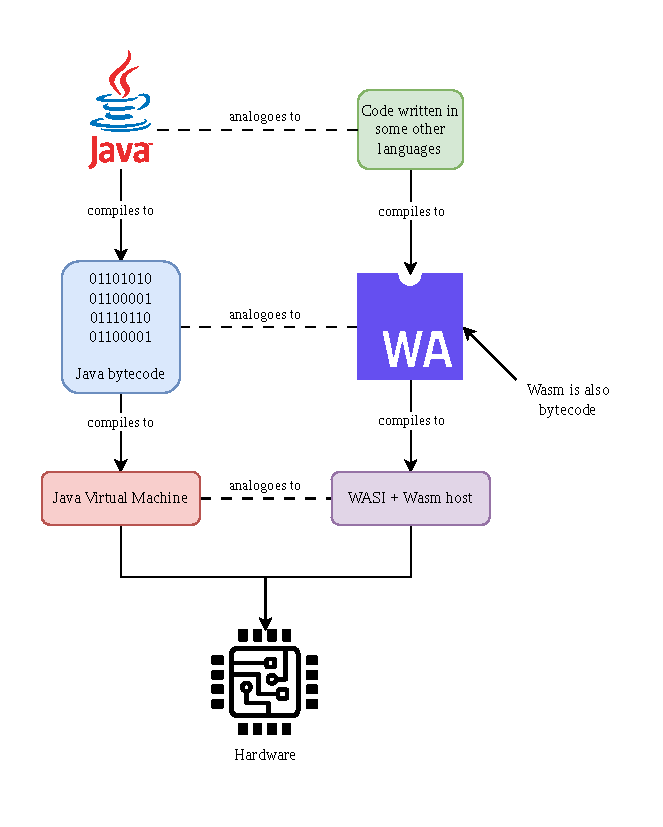
\includegraphics[width=0.7\textwidth]{figures/java_vs_wasm.pdf}
    \caption{An analogy comparing the cross-platform execution models of Java and WebAssembly. Adapted from Chiarlone \cite{chiarlone2024serverside}.}
    \label{fig:java_vs_wasm}
\end{figure}

For languages requiring automatic memory management (like Go, Python, Kotlin, or PHP), Wasm historically required the entire language runtime and garbage collector to be compiled and bundled inside the \texttt{.wasm} binary. This approach bloated the deployment artifact and created redundant layers of memory management. For instance, deploying a compiled-to-Wasm language with its own garbage collector into a host environment that already possesses one (such as a browser engine like V8) is highly wasteful \cite{steiner2023wasmgc}. Furthermore, having no interaction between Wasm's linear memory and the built-on-top garbage collector of the ported language often caused problems like memory leaks and inefficient collection attempts \cite{liedtke2023v8wasmgc}.

To resolve this, the WebAssembly Garbage Collection (WasmGC) standard has been introduced to delegate memory management directly to the host environment. WasmGC extends the WebAssembly memory model by adding struct and array heap types, thereby providing native support for non-linear memory allocation \cite{wasm2023gcproposal}. Because each WasmGC object has a fixed type and structure, host VMs can generate highly efficient access code without the risk of dynamic deoptimizations. This allows higher-level managed languages to bypass bundling their own garbage collectors, instead interfacing efficiently with the host VM's built-in garbage collector.

The architectural impact on artifact density is significant. By eliminating the need to bundle memory management code, WasmGC binaries for managed languages can achieve dramatically smaller footprints. In early benchmarks, WasmGC binaries for languages like Java were proven to be considerably smaller than equivalent modules compiled from C or Rust, because C and Rust must still bundle manual memory management routines like \texttt{malloc} and \texttt{free} inside the binary \cite{steiner2023wasmgc}. This advancement firmly positions Wasm as a viable, high-density target for the entire spectrum of modern programming languages.

\subsection{The Server-Side Evolution: WASI}
While Wasm successfully delivered near-native performance for computationally heavy browser applications, its portability, mathematical security model, and minimal footprint rapidly garnered interest for backend deployment. Solomon Hykes, the founder of Docker, once famously stated: 
\begin{quote}
    If WASM+WASI existed in 2008, we wouldn't have needed to create Docker. That's how important it is. WebAssembly on the server is the future of computing. ~\cite{hykes2019tweet}
\end{quote}
 
Because Wasm is entirely isolated by default, a bare Wasm module running on a server cannot open a network socket, read a file, or query the system clock. In 2019, the WebAssembly System Interface (WASI) was introduced to solve this. WASI defines a standardized API specification that provides Wasm modules with secure, granular, capability-based access to the host operating system ~\cite{clark2019standardizing}. By acting as a secure POSIX-like layer, WASI transforms Wasm from a sandboxed browser calculator into a fully functional server-side technology.

\subsection{Capability-Based Security Model}
WASI implements a capability-based security model that diverges significantly from traditional Linux permissions.  A Linux container limits an already-running OS environment. WASI, however, enforces a strict "deny-by-default" posture. 

If a Wasm module needs to access a configuration file, it cannot invoke a standard `open()` system call for an arbitrary path (e.g., `/etc/config`). Instead, the host runtime must explicitly grant the module a "pre-opened" file descriptor at startup. The module is completely blind to the existence of the host filesystem outside the specific directory tree explicitly mapped and passed to it by the runtime.

\begin{figure}[htbp]
    \centering
    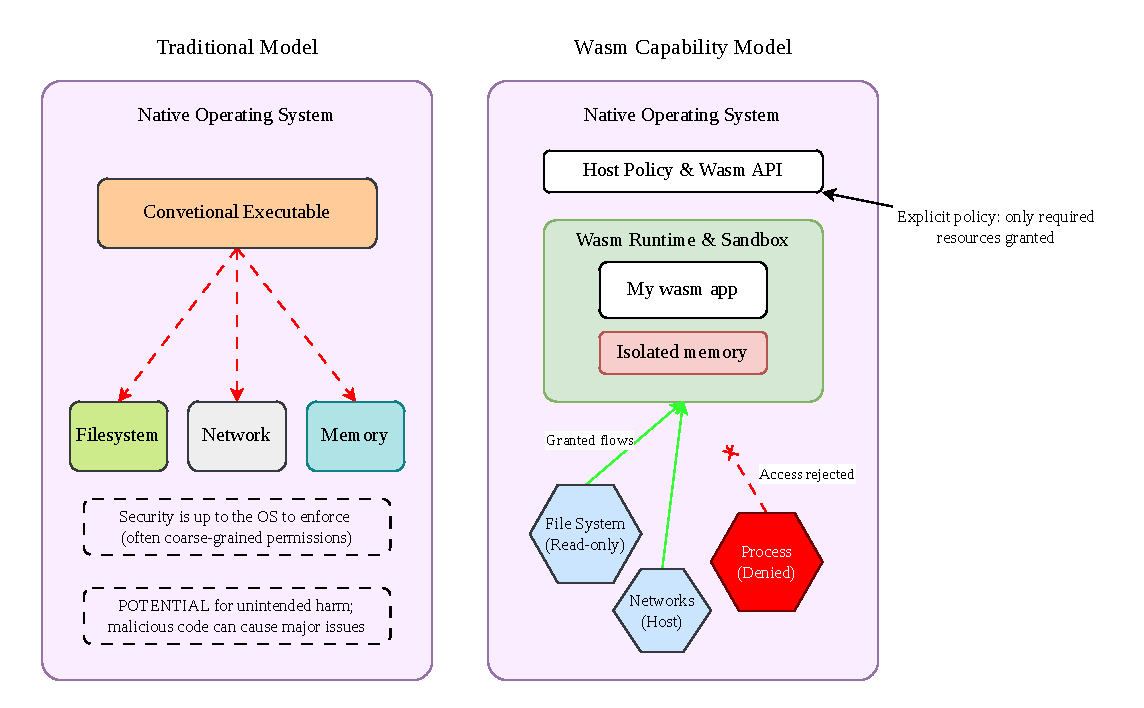
\includegraphics[width=\textwidth]{figures/wasm_sandboxed_model.pdf}
    \caption{Comparative Security Models: Traditional vs Wasm Capabilities}
    \label{fig:wasm_sandboxed_model}
\end{figure}

\subsection{Architectural Evolution: From POSIX to the Component Model}
The initial iteration of WASI (often referred to as WASI Preview 1) was heavily modeled after standard POSIX interfaces, focusing on file descriptors, environment variables, and standard I/O streams. While effective for simple command-line tools and basic microservices, this POSIX-centric approach introduced friction when handling complex, multi-language cloud-native interactions.

To address this, the WebAssembly ecosystem is currently transitioning to the WebAssembly Component Model (WASI Preview 2 and Preview 3).  The Component Model shifts WASI from a low-level POSIX API to a high-level, language-agnostic interface system utilizing WebAssembly Interface Types (WIT). This advancement allows discrete Wasm components—potentially written in entirely different source languages—to natively interoperate. They can securely pass complex data types (such as strings, records, and variants) across execution boundaries without sharing linear memory, laying the foundation for highly modular, secure, and dynamically composable microservice architectures.

\subsection{Wasm vs. Traditional Containers}
Applying Wasm and WASI to the server yields a deployment artifact that sits functionally between a traditional VM and an OCI container, offering unique operational characteristics:

\begin{enumerate}
    \item \textbf{Cold Start and Footprint:} Traditional OCI containers bundle an OS userland, frequently resulting in image sizes exceeding 100MB and startup times measured in seconds. A Wasm module contains only the compiled application logic. Wasm binaries are typically just a few megabytes and can be instantiated by a host runtime in microseconds. Long et al. demonstrated that Wasm runtimes can perform at least 10x faster than Docker from a cold start for short-running workloads ~\cite{long2023wasm}. Hall and Ramachandran further verified that Wasm's improved cold start times lead to up to 90\% faster response times for basic serverless tasks ~\cite{hall2021serverless}.
    \item \textbf{Security and Density:} Wasm utilizes Software-Based Fault Isolation (SFI). If a Wasm module is compromised, the attacker only controls the isolated linear memory sandbox. Because Wasm threads do not require full OS process overhead, the minimal memory footprint allows Kubernetes nodes to achieve exponentially higher workload density.
    \item \textbf{Performance Trade-offs:} Despite its advantages in density and initialization, Wasm remains structurally immature compared to Docker regarding concurrency. Wasm currently lacks robust, standardized multithreading capabilities (the Wasm Threads proposal relies on shared memory buffers that complicate isolation). Sondell (2024) demonstrated that in high-concurrency HTTP server scenarios, a Docker container can process requests significantly faster because it can scale natively across multiple CPU cores, whereas a single Wasm instance frequently remains bottlenecked by single-threaded execution ~\cite{sondell2024performance}. Furthermore, Spies and Mock found that single-threaded Wasm apps perform approximately 14\% slower than native x86\_64 binaries due to sandbox bounds-checking overhead ~\cite{spies2021evaluation}.
\end{enumerate}

By utilizing WASI shims (such as \texttt{runwasi}), Kubernetes can now orchestrate these high-density Wasm workloads directly alongside traditional Docker containers, establishing the precise technological foundation for the comparative analysis executed in this research.
\chapter{Related Work}
\label{chap:state_of_the_art}

This chapter surveys the academic literature and industry evidence most directly relevant to the research questions of this thesis. Section~\ref{sec:academic_research} reviews quantitative performance studies comparing server-side \acs{Wasm} and container workloads, security analyses contrasting \acs{Wasm}'s isolation model with Docker's kernel-sharing model, and compiler strategy trade-offs identified in prior work. Section~\ref{sec:industry_landscape} surveys the current commercial deployment landscape of server-side \acs{Wasm} across edge computing providers and application frameworks. Section~\ref{sec:wasm_in_production} presents concrete production deployments and ecosystem maturity evidence. Technical background on the \acs{Wasm} Component Model, available runtimes, and the \acs{K8s} integration landscape is provided in \hyperref[chap:background]{Chapter~\ref{chap:background}}.

\section{Academic Research and Benchmarks}
\label{sec:academic_research}

The following section surveys peer-reviewed and academic work that measures or analyses the performance, security, and ecosystem properties of server-side \acs{Wasm} relative to container-based alternatives. These studies provide the empirical baseline against which the results of this thesis are positioned and contextualised. The section is structured as follows: Section~\ref{sec:performance_studies} covers quantitative performance benchmarks; Section~\ref{sec:security_comparisons} examines security analyses; Section~\ref{sec:jit_vs_aot} discusses compiler strategy trade-offs documented in prior work.

\subsection{Performance Studies}
\label{sec:performance_studies}

Several academic works have investigated the performance characteristics of server-side \acs{Wasm} and directly inform the research questions of this thesis. The studies below are grouped by the performance dimension they address: native-binary overhead, cold-start and density advantages, and throughput under concurrent load.

\textit{Native-binary overhead.}\quad \textcite{jangda2019notsofast} performed a systematic analysis of \acs{Wasm} performance relative to native x86\_64 code across a broad set of benchmarks from the PolyBenchC suite. They found that \acs{Wasm} is on average 1.5$\times$ slower than native code, with the overhead attributable to \acs{SFI} bounds-checking, function pointer masking, and the inability of the \acs{Wasm} \acs{ABI} to exploit all available hardware registers. Separately, \textcite{spies2021evaluation} evaluated \acs{Wasm} compiled with \texttt{wasm32-wasi} in non-web environments and found that single-threaded, \acs{CPU}-bound workloads run approximately 14\% slower than equivalent native x86\_64 binaries~\cite{spies2021evaluation}. This overhead stems from the bounds-checking and indirect-call guards enforced at runtime by \acs{SFI}. Their study establishes an important baseline: the \acs{Wasm} runtime is not free of overhead even for compute-intensive tasks, though the gap shrinks considerably with \ac{AOT} compilation.

\textit{Cold-start latency and image density.}\quad \textcite{long2023wasm} conducted a direct performance comparison between \acs{Wasm} and containerized workloads, demonstrating that \acs{Wasm} runtimes achieve at least a 10$\times$ improvement in cold-start latency over Docker for short-running workloads. This advantage is most pronounced in \acl{FaaS} scenarios where containers are created and destroyed frequently. \textcite{hall2021serverless} extended this finding to the serverless domain, showing that the \acs{Wasm} cold-start advantage translates into up to 90\% faster end-to-end response times for event-driven serverless functions~\cite{hall2021serverless}. Importantly, both of these cold-start advantages are primarily attributable to \acs{Wasm}'s dramatically smaller deployment artifacts rather than to fundamental differences in \ac{JIT} compilation speed alone.

\textit{Concurrent throughput.}\quad The most directly comparable prior work to this thesis is the master's thesis by \textcite{sondell2024performance} at \acs{KTH} Royal Institute of Technology. Sondell benchmarked \acs{Wasm} containers against Docker containers for serverless \acs{HTTP} workloads and found a significant throughput collapse under concurrent load for the \acs{Wasm} variant. The root cause is identical to the finding documented in this thesis: \acs{WASI}~Preview~1 does not expose thread-spawning primitives to modules, leaving the \acs{HTTP} server constrained to processing one request at a time while Docker containers leverage native multi-core concurrency via goroutines or thread pools. Sondell's work uses a different runtime configuration and workload type; this thesis extends that line of inquiry with four implementation variants (two language families, two runtime targets), a dedicated \acs{CPU}-bound compute benchmark, and a structured developer experience assessment, providing complementary empirical coverage of the \acs{Wasm}/\acs{K8s} deployment space.

\subsection{Security Comparisons}
\label{sec:security_comparisons}

The security architecture of \acs{Wasm}/\acs{WASI} has been studied in the context of multi-tenant cloud workloads, with analyses focusing on both the structural advantages of \acs{Wasm}'s isolation model and its residual attack surface.

\textit{Container security risks.}\quad \textcite{combe2016docker} surveyed the security properties of Docker and found that the shared-kernel model is the primary structural risk in multi-tenant deployments. If a container escape vulnerability is exploited, the attacker gains code execution at the host kernel level, potentially compromising every container on the node. Shillaker and Pietzuch similarly documented the kernel-sharing threat model in the context of serverless isolation~\cite{shillaker2020faasm}: a single compromised container can expose the entire host to privilege escalation. \acs{Wasm}, by contrast, enforces \acs{SFI} at the runtime level: the module can only read and write within its allocated linear memory region, and any out-of-bounds access results in a deterministic, immediate trap. A module compromise therefore yields only control of that module's sandboxed linear memory, not host-level execution.

\textit{Wasm binary security.}\quad \textcite{lehmann2020everythingold} analysed the binary security properties of \acs{Wasm} modules and found that, while the linear memory model successfully prevents classical memory-safety attacks (buffer overflows, use-after-free), it introduces a new class of confused-deputy vulnerabilities at the Wasm-host interface boundary. Specifically, if a host import (a function provided by the runtime to the \acs{Wasm} module) is overly permissive, an attacker with control over the module can abuse it to perform operations outside the intended capability scope. This finding is directly relevant to the experimental setup in this thesis: the use of \texttt{wasmedge\_wasi\_socket}, a \acs{WasmEdge}-specific extension that grants the module full \acs{TCP} socket access, is an example of a permissive host import. Fine-grained network capability restriction---the theoretical security advantage of \acs{WASI}'s deny-by-default model---is therefore not exercised in the benchmarks.

\acs{WASI} extends the isolation model with a \ac{POLA}-based capability model: network sockets, files, and environment variables are only accessible if the host runtime explicitly grants them at startup. This ``deny-by-default'' posture is structurally more restrictive than Linux's permission model, though as the findings above illustrate, its practical security benefit depends on how conservatively host imports are defined.

\subsection{JIT vs.\ AOT Compilation}
\label{sec:jit_vs_aot}

\acs{Wasm} runtimes offer two primary compilation strategies that directly affect the cold-start vs.\ throughput trade-off, and this choice has been studied in the context of both browser and server-side deployments.

\ac{JIT} compilation---the default mode in \acs{WasmEdge}---translates the \texttt{.wasm} binary to native machine code at module load time. This preserves binary portability across \acs{ISA}s and keeps the deployment artifact small, at the cost of a one-time JIT overhead on first pod startup. \ac{AOT} compilation pre-translates the \texttt{.wasm} binary to a platform-specific native shared object before deployment, eliminating the JIT startup penalty entirely but tying the artifact to a specific architecture. \textcite{spies2021evaluation} showed that the performance gap between \acs{Wasm} and native code narrows considerably under \acs{AOT} compilation, suggesting that JIT overhead is a significant but avoidable contributor to the 14\% slowdown they observed. \acs{WasmEdge} supports \acs{AOT} via its \texttt{wasmedgec} \acs{CLI} tool.

This thesis uses the \acs{JIT} path for both \acs{Wasm} variants to maintain binary portability and reproducibility across potential future cluster migrations. This is acknowledged as a conservative choice that may slightly disadvantage the \acs{Wasm} variants in the compute benchmark; \acs{AOT} compilation is left as a direction for future optimisation work.

\section{Industry Adoption of Server-Side WebAssembly}
\label{sec:industry_landscape}

This section maps the current commercial deployment landscape of server-side \acs{Wasm}. Understanding where \acs{Wasm} has already been deployed at production scale provides essential context for interpreting the benchmark results in Chapter~\ref{chap:evaluation} and for calibrating expectations about ecosystem maturity.

\subsection{Edge Computing Providers}

The first large-scale production deployments of server-side \acs{Wasm} occurred at edge computing providers, where cold-start density and instantiation latency are primary commercial constraints.

\textbf{Cloudflare Workers}~\cite{cloudflare2024workers} runs \acs{Wasm} inside V8 Isolates---not a \acs{WASI} runtime---by embedding the browser's JavaScript engine at the network edge. Each Worker invocation receives a fresh V8 Isolate with sub-millisecond startup across a network spanning 310+ cities in 120+ countries. This model proves that \acs{Wasm}'s density advantages are commercially viable at hyperscale, though the V8 Isolate isolation mechanism differs from the \acs{WASI}-based server-side deployments studied in this thesis.

\textbf{Fastly Compute}~\cite{fastly2024compute} built its edge computing platform on Lucet, an \acs{AOT}-compiling \acs{Wasm} runtime developed internally. Rather than replacing Lucet outright, Fastly subsequently migrated its key innovations---the \acs{AOT} compilation pipeline and the pooling allocator---into Wasmtime, the Bytecode Alliance's reference runtime~\cite{fastly2020lucetwasm}. Fastly Compute now runs on Wasmtime in production, demonstrating both the commercial maturity of the \acs{Wasm} runtime ecosystem and a broader pattern of vertical implementations converging toward the shared Bytecode Alliance reference.

\subsection{Application Frameworks and Platforms}

\textbf{Fermyon Spin}~\cite{fermyon2024spin} is a developer-centric framework for building serverless \acs{Wasm} microservices. Spin uses a request-scoped execution model: a fresh \acs{Wasm} instance is created per \acs{HTTP} request and destroyed upon response. This model maximises cold-start density and isolates request state, but is architecturally opposite to the persistent \acs{TCP} server approach used in this thesis. Spin targets \acs{WASI}~P1 and is actively migrating to \acs{WASI}~P2's \texttt{wasi:http} world.

\textbf{WasmCloud}~\cite{wasmcloud2024} is an actor-model distributed application platform. Services are implemented as location-transparent actors that communicate over a \acs{NATS} message bus; the runtime injects capability providers for networking, databases, and other host resources at launch time without baking them into the actor binary. WasmCloud targets the \acs{WASI}~P2 Component Model and is a \acs{CNCF}-sponsored project. Its distributed-systems orientation makes it a strong candidate for the Volta microservice architecture planned as future work in this thesis.

\textbf{WasmEdge}~\cite{cncf2024wasmedge} is a general-purpose runtime that supports long-running \acs{TCP} servers, multiple language targets (Rust, TinyGo, C/C++, Python), and a \acs{containerd} shim for \acs{K8s} \texttt{RuntimeClass} integration. These properties make it the runtime of choice for this thesis; the detailed selection rationale is presented in Section~\ref{sec:runtime_landscape}.

\section{Server-Side WebAssembly in Production}
\label{sec:wasm_in_production}

This section presents concrete evidence of server-side \acs{Wasm} deployments at production scale, focusing on quantifiable milestones and ecosystem governance signals that indicate the technology's maturity relative to the experimental deployment studied in this thesis.

\subsection{Cloudflare Workers at Scale}

Cloudflare Workers is the largest publicly documented deployment of server-side \acs{Wasm} to date~\cite{cloudflare2024workers}. The platform executes customer-authored \acs{Wasm} modules across 310+ points of presence globally, isolating each invocation in a V8 Isolate with cold-start overhead measured in single-digit milliseconds. Cloudflare's 2025 ``Shard and Conquer'' architecture further reduced cold starts to the point where 99.99\% of requests are served warm, effectively eliminating cold-start penalty as a user-visible phenomenon at their scale of operation.

The relevance to this thesis is two-fold. First, the platform demonstrates that \acs{Wasm}'s density advantage---many isolated tenants per host, with rapid instantiation---is not merely theoretical but commercially proven at global scale. Second, the isolation mechanism (V8 Isolates rather than a \acs{WASI} runtime) highlights that production-grade \acs{Wasm} deployments can diverge significantly in their security and capability models; the \acs{WASI}-based approach evaluated in this thesis represents a different, \acs{K8s}-native deployment pattern.

\subsection{Fastly and the Convergence to Wasmtime}

Fastly's trajectory from Lucet to Wasmtime illustrates a broader pattern of ecosystem consolidation~\cite{fastly2020lucetwasm, fastly2024compute}. When Fastly open-sourced Lucet in 2019 as a production-grade \acs{AOT} \acs{Wasm} compiler and runtime, it represented the state of the art for serverless \acs{Wasm} performance. As the Bytecode Alliance's Wasmtime matured, Fastly contributed Lucet's key innovations---including the pooling instance allocator and \acs{AOT} ahead-of-time compilation pipeline---directly into the shared Wasmtime codebase, then migrated Fastly Compute to run on Wasmtime.

This convergence is significant from an ecosystem perspective: even a well-funded, production-grade custom runtime found it strategically preferable to merge into the community reference implementation rather than maintain a divergent fork. The result is a stronger shared base for all \acs{Wasm} runtimes and evidence that the Bytecode Alliance governance model produces long-term ecosystem stability---a factor relevant to any organisation evaluating a migration to \acs{Wasm}-based infrastructure.

\subsection{CNCF Ecosystem Maturity}

The governance investment by the \acs{CNCF} in server-side \acs{Wasm} projects provides a quantifiable maturity signal. \acs{WasmEdge} was accepted into the \acs{CNCF} Sandbox on 28 April 2021~\cite{cncf2024wasmedge}---the same maturity track used by Kubernetes, containerd, and Prometheus before they graduated. SpinKube, the \acs{K8s} operator for running Fermyon Spin applications natively, entered the \acs{CNCF} Sandbox on 21 January 2025~\cite{spinkube2024}. runwasi, the Rust library for writing containerd shims for \acs{Wasm} workloads, is actively maintained under the containerd organisation and is used in production by both K3s~\cite{k3s2024rancher} and Microsoft's Azure Kubernetes Service to execute \acs{Wasm} workloads via \texttt{RuntimeClass}~\cite{runwasi2024}. The \acs{CNCF} TAG-Runtime \acs{Wasm} Working Group~\cite{cncf2024tagruntime} was chartered to define best practices for \acs{Wasm} as a first-class cloud-native workload type alongside \acs{OCI} containers.

Collectively, these governance milestones indicate that server-side \acs{Wasm} has crossed from a research curiosity to an infrastructure category with active stewardship by the same foundation that governs the broader cloud-native ecosystem. This is directly relevant to this thesis: \acs{WasmEdge} and K3s---both \acs{CNCF}-affiliated projects---are the two primary runtime components used in the experimental cluster.

\chapter{Research Methodology}
\label{chap:methodology}

This chapter describes the research strategy employed to compare \acs{Wasm} and Docker-based microservice deployments, justifies the selection of the four implementation variants, defines the four benchmark workloads, and specifies the six measurement metrics used throughout the evaluation.

\section{Research Strategy}
\label{sec:research_strategy}

This thesis employs a \textit{mixed-methods} approach combining a quantitative controlled experiment as the primary method with a qualitative developer experience assessment as the secondary method.

The primary quantitative experiment follows a 2$\times$2 variant matrix: runtime (Docker/\texttt{runc} vs.\ \acs{Wasm}/SpinKube) crossed with language family (Rust vs.\ Go-family). This produces four primary implementation variants deployed to an isolated, reproducible cloud environment and subjected to identical load testing and startup-time measurements. All variants implement the same \acs{HTTP} \acs{API} and the same core algorithm, ensuring that any performance difference is attributable to the execution environment rather than to differences in application logic. The benchmark source code, k6 load-generator scripts, and raw result data are openly available in the \texttt{thesis-experiments} repository~\cite{musaev2026thesisexperiments}.

The \acs{Wasm} variants use the standardised \texttt{wasi:http/incoming-handler} Component Model interface (\acs{WASI}~P2) via Fermyon Spin and Wasmtime/Cranelift. This design choice reflects the current production-ready trajectory of \acs{Wasm} on \acs{K8s}: the \acs{WASI}~P2 Component Model provides a standards-compliant \acs{HTTP} handler interface, replacing the proprietary socket workarounds historically required under \acs{WASI}~P1.

An important design choice is that this study does \textit{not} attempt to isolate the pure runtime overhead by holding the language constant across all four variants. Instead, it deliberately compares the two dominant paradigms in their \textit{native} technological contexts: Docker with Go (the industry standard), Docker with Rust (a deconfounding baseline), and \acs{Wasm} with Rust and TinyGo (the \acs{Wasm}-native ecosystem). This design reflects the real-world decision an engineering team faces when evaluating a migration from Docker to \acs{Wasm}, while the Rust-on-Docker baseline enables partial deconfounding of the language variable (see Section~\ref{sec:tech_selection}).

\section{Selection of Technologies}
\label{sec:tech_selection}

\subsection{Docker/Golang: The Industry Baseline}

The Docker/Golang variant serves as the primary baseline against which all other variants are measured. Go is the de facto language for cloud-native infrastructure tooling: \acs{K8s}~\cite{burns2016borg}, Docker~\cite{merkel2014docker}, Terraform~\cite{terraform2024hashicorp}, Prometheus~\cite{prometheus2024cncf}, and Grafana are all implemented in Go. Its goroutine-based concurrency model and the \texttt{net/http} standard library make it the idiomatic choice for \acs{HTTP} microservices. Among production-grade garbage-collected languages, Go offers competitive raw throughput while retaining ergonomic memory safety, making it a strong baseline for evaluating whether \acs{Wasm}'s elimination of bundled garbage collection overhead provides a meaningful performance advantage.

\subsection{Docker/Rust: The Deconfounding Baseline}

A second Docker-based baseline using Rust is included specifically to enable a language-controlled comparison. Because both docker-rust and wasm-rust use the same language, the performance delta between these two variants isolates (approximately) the overhead introduced by the SpinKube/Wasmtime runtime, \acs{SFI} bounds-checking, and the single-instance dispatch constraint imposed by the \texttt{SpinApp~spec.replicas:~1} limited-mode baseline (each \acs{WASI} P1/P2 component is architecturally single-threaded), independent of language-level differences such as memory management strategy.

Rust's axum/Tokio async stack provides full multi-threaded, asynchronous I/O---the maximum performance achievable on the Docker/\texttt{runc} path---making the docker-rust variant also a useful upper-bound reference for the \acs{Wasm} variants.

\subsection{Wasm/Rust: The Primary Experimental Variant}

\acs{Wasm} supports more than 40 programming languages as compilation targets~\cite{fermyon2024langmatrix}. Rust was selected as the primary \acs{Wasm} experimental language for three reasons. First, Rust provides first-class, officially supported \texttt{wasm32-wasip1} and \texttt{wasm32-wasip2} targets maintained by the Rust core team; \texttt{wasm32-wasip2} has been Tier~2 stable since Rust~1.82~\cite{rustblogwasip2}. Second, Rust produces the smallest \acs{Wasm} binaries among systems languages because it has no garbage collector, no language runtime, and no \acs{OS} abstraction layer bundled into the binary. Third, the Spin \acs{SDK} for Rust (\texttt{spin-sdk~=~"5.2.0"}) provides a first-class \texttt{\#[http\_component]} macro that generates a standards-compliant \acs{WASI}~P2 component with no custom networking code.

The wasm-rust variant uses \texttt{cargo component build --release} (via \texttt{cargo-component}) to compile to a \acs{WASI}~P2 component. The resulting \texttt{.wasm} binary is published as a Spin \acs{OCI} artifact via \texttt{spin registry push}. Spin's Wasmtime/Cranelift host handles the \acs{HTTP} listener, request parsing, and response dispatch---the component itself exports only a single handler function, eliminating any need for manual \acs{TCP} socket management.

\subsection{Wasm/TinyGo: The Secondary Experimental Variant}

TinyGo~\cite{tinygo2024} is a Go-compatible compiler optimised for embedded systems and \acs{Wasm} targets. It was selected to enable a partial Go-to-Go comparison with the docker-golang baseline, testing whether the concurrency model difference between Docker's goroutine scheduler and \acs{Wasm}'s request-handler model produces measurable performance differences when the language is held constant.

Standard Go supports \texttt{GOOS=wasip1} since Go~1.21~\cite{goblogwasi2024}, but produces significantly larger \acs{Wasm} binaries because it bundles the full Go runtime (scheduler, garbage collector, and \acs{POSIX} abstraction layer). TinyGo is designed specifically for \acs{Wasm}/embedded targets and produces substantially smaller binaries by using a stripped-down runtime. TinyGo~0.40.0 targeting \texttt{wasip1} was pinned for this experiment.

The wasm-tinygo variant uses \texttt{spinhttp.Handle()} from the official Spin \acs{SDK} for Go (\texttt{github.com/spinframework/spin-go-sdk/v2}). The handler function receives standard \texttt{net/http.ResponseWriter} and \texttt{*http.Request} arguments---identical to the docker-golang handler. \textbf{No custom socket code is required.} TinyGo's \texttt{-target=wasip2} flag cannot be used here: it hardwires the \texttt{wasi:cli/command} world and cannot export \texttt{wasi:http/incoming-handler}. The Spin Go \acs{SDK} uses a \acs{CGo} layer to export \texttt{fermyon:spin/inbound-http}, which Spin/Wasmtime accepts as a valid \acs{HTTP} trigger interface. The \texttt{-target=wasip1} flag is therefore required.

\subsection{Orchestration: Kubernetes (kubeadm) with RuntimeClass}

Upstream Kubernetes v1.34, deployed via \texttt{kubeadm}, was chosen as the orchestration layer. \texttt{kubeadm} is the reference installer in the official Kubernetes documentation and the foundation that managed services such as \acs{AWS} \acs{EKS}, Google \acs{GKE}, and Azure \acs{AKS} run underneath; using it removes distribution-specific confounds from the runtime comparison. The benchmark \acs{VM} is sized at Hetzner Cloud \texttt{ccx23} (4 dedicated \acs{AMD} \acs{EPYC} vCPUs, 16\,\acs{GB} \acs{RAM}, 160\,\acs{GB} \acs{NVMe}) to give the kubeadm control plane, the kube-prometheus-stack observability stack, the SpinOperator, and the unlimited-mode scaling experiment comfortable headroom on a single node. kubeadm uses containerd~2.x as its \acs{CRI}, which is necessary for the \texttt{RuntimeClass}/SpinKube integration; Flannel provides the pod-network \acs{CNI} and Rancher's \texttt{local-path-provisioner} provides the default \texttt{StorageClass} for the Prometheus \acs{PVC}.

The \acs{Wasm} \texttt{RuntimeClass} (\texttt{wasmtime-spin}) routes pods to \texttt{containerd-shim-spin-v2}~v0.17.0, which embeds Spin and Wasmtime/Cranelift internally to execute \acs{WASI}~P2 components. Docker pods use the default \texttt{runc} path unchanged. This hybrid configuration allows both paradigms to run side-by-side with directly comparable \acs{K8s} resource management.

\section{Benchmark Workload Design}
\label{sec:workload_design}

\subsection{Sieve of Eratosthenes as the Compute Benchmark}

The first benchmark workload is a stateless \acs{HTTP} service that computes prime numbers using the Sieve of Eratosthenes algorithm. The sieve was selected as the opening benchmark for several reasons. It is purely \acs{CPU}-bound with no external I/O, database calls, or file system access, isolating compute performance from I/O stack differences between the variants. Its $O(N \log \log N)$ time complexity produces a predictable, parametrically controllable workload: the upper bound $N$ can be adjusted to modulate per-request computation time precisely. The algorithm is deterministic and trivially re-implementable in any language, ensuring that all six variants compute identical results using the same algorithmic logic.

The \acs{HTTP} \acs{API} contract is identical across all six variants:

\begin{verbatim}
GET /prime?limit=N&no_list=1
\end{verbatim}

The response is a \acs{JSON} object:
\begin{verbatim}
{"runtime":"<variant>","limit":N,"count":K,"elapsed_us":T}
\end{verbatim}

The \texttt{no\_list=1} parameter suppresses the array of computed primes from the response body, eliminating \acs{JSON} serialization overhead as a confounding variable when measuring throughput. The \texttt{elapsed\_us} field records the server-side wall-clock time of the sieve computation in microseconds, providing a direct measurement of per-request algorithmic cost independent of network and queuing latency.

Table~\ref{tab:variant_summary} summarizes the four primary implementation variants.

\begin{table}[htbp]
    \centering
    \caption{Summary of the four primary benchmark variants}
    \label{tab:variant_summary}
    \adjustbox{max width=\linewidth}{%
    \begin{tabular}{llllll}
        \hline
        \textbf{Variant} & \textbf{Language} & \textbf{Runtime} & \textbf{Framework} & \textbf{I/O Model} & \textbf{NodePort} \\
        \hline
        wasm-rust     & Rust~1.94     & Wasmtime/Cranelift & \texttt{spin-sdk} \texttt{\#[http\_component]} & \acs{WASI}~P2 handler  & 30081 \\
        wasm-tinygo   & TinyGo~0.40.0 & Wasmtime/Cranelift & \texttt{spinhttp.Handle()}  & Spin HTTP (\acs{WASI}~P1 via CGo) & 30082 \\
        docker-rust   & Rust~1.94     & runc          & axum + Tokio                & Async (multi-thread)      & 30083 \\
        docker-golang & Go~1.26       & runc          & \texttt{net/http}           & Goroutines (M:N)          & 30084 \\
        \hline
    \end{tabular}}
\end{table}

\subsection{Memory-Bandwidth Benchmark}
\label{sec:memory_bandwidth_workload}

The second benchmark workload is a stateless \acs{HTTP} service that allocates an in-memory buffer of configurable size, fills it with deterministic bytes, computes its \acs{SHA}-256 hash, and returns the hash and elapsed time. This workload was designed to contrast with the \acs{CPU}-bound prime sieve by stressing memory-allocation patterns and the runtime's ability to handle repeated large-heap operations.

\textit{Note on filesystem I/O:} The original design called for writing to and reading from a temporary file. However, SpinKube's Wasmtime host exposes \texttt{wasi:filesystem} access only to explicitly declared directories in \texttt{spin.toml}; ephemeral \texttt{/tmp} writes are not available in the default SpinApp sandbox. The in-memory buffer approach provides an equivalent memory-pressure workload that is consistent across all four variants (Docker variants perform the same in-memory computation without filesystem involvement), preserving the fairness of the comparison.

The \acs{HTTP} \acs{API} contract is identical across all four variants:

\begin{verbatim}
GET /membw?size_kb=N&no_hash=0
\end{verbatim}

The response is a \acs{JSON} object:
\begin{verbatim}
{"runtime":"<variant>","size_kb":N,"sha256":"<hex>","elapsed_us":T}
\end{verbatim}

The \texttt{no\_hash=1} parameter suppresses the hash computation (returning an empty string), enabling measurement of raw allocation overhead independently of hashing time. Default \texttt{size\_kb=64}; maximum \texttt{size\_kb=10240}. The benchmark uses \texttt{size\_kb=64} for load testing and \texttt{size\_kb=1024} for stress testing large-allocation behaviour.

\subsection{HTTP Fan-out Benchmark (I/O-Bound)}
\label{sec:http_fanout_workload}

The third benchmark workload is the \textit{I/O-bound} counterpart promised in the task description. Each variant exposes an \acs{HTTP} service that, on every inbound request, dispatches $N$ concurrent outbound \acs{HTTP} GETs to an in-cluster delay-injecting backend pod (\texttt{io-echo}) and aggregates the responses. The backend sleeps for \texttt{delay\_ms} before responding, so per-request latency is dominated by outbound I/O wait rather than \acs{CPU} work --- the workload is I/O-bound by construction. The \texttt{io-echo} pod is intentionally \textit{not} part of the comparison matrix; it is a stable I/O target whose response delay and payload size are tunable parameters, turning variation in the inbound-side measurements into a runtime-and-language signal rather than backend noise.

The \acs{HTTP} \acs{API} contract is identical across all four variants:

\begin{verbatim}
GET /fanout?n=N&delay_ms=D&no_list=0|1
\end{verbatim}

The response is a \acs{JSON} object:
\begin{verbatim}
{"runtime":"<variant>","n":N,"delay_ms":D,
 "ok_count":K,"err_count":E,"elapsed_us":T,"responses":[...]}
\end{verbatim}

Defaults: \texttt{n=5}, \texttt{delay\_ms=50}, \texttt{no\_list=1} during load tests (the \texttt{responses} array is omitted to eliminate response-serialization overhead as a confounding variable). The \texttt{elapsed\_us} field measures wall-clock time from the first outbound dispatch through the last response, excluding inbound \acs{HTTP} framing.

\textit{Concurrency model per variant.} The wasm-rust variant fans out concurrently via \texttt{spin\_sdk::http::send} composed with \texttt{futures::future::join\_all}; docker-rust uses \texttt{reqwest::Client} with the same \texttt{join\_all} pattern; docker-golang uses \texttt{net/http} with \texttt{sync.WaitGroup} over goroutines. The wasm-tinygo variant, however, dispatches the $N$ outbound \acs{HTTP} GETs \textit{sequentially}: TinyGo's wasip1 runtime panics on \texttt{sync.WaitGroup.Wait()} (nil-pointer dereference in the goroutine scheduler), and \texttt{spinhttp.Send} itself is blocking per call. This asymmetry --- three variants can fan out concurrently but the fourth cannot under WASI~P1 --- is itself a thesis-relevant observation about the maturity of the Wasm side for I/O-heavy workloads (see Section~\ref{sec:discussion_fanout}).

The Spin variants gate outbound \acs{HTTP} via \texttt{allowed\_outbound\_hosts~=~[\textquotedbl http://io-echo.http-fanout.svc.cluster.local:80\textquotedbl ]} in \texttt{spin.toml}, reflecting Spin's idiomatic deny-by-default capability model. The same gating is unavailable on the Docker side, which is itself a security-posture qualitative observation (Chapter~\ref{chap:discussion}).

\subsection{JSON Round-trip Benchmark (Serialization + Allocator)}
\label{sec:json_roundtrip_workload}

The fourth benchmark workload stresses the \textit{serialization and allocator hot path} that none of the previous three workloads exercise. Each variant exposes an \acs{HTTP} service that accepts a posted \acs{JSON} integer array, parses it, sorts it descending, computes aggregate statistics (count, sum, min, max, mean, median, standard deviation), and returns the aggregates as \acs{JSON}.

The \acs{HTTP} \acs{API} contract is identical across all four variants:

\begin{verbatim}
POST /jsontx?n=N&no_list=0|1
Content-Type: application/json
Body: [a, b, c, ...]  (array of N integers)
\end{verbatim}

The response is a \acs{JSON} object containing \texttt{runtime}, \texttt{n}, \texttt{count}, \texttt{sum}, \texttt{min}, \texttt{max}, \texttt{mean}, \texttt{median}, \texttt{stdev}, \texttt{elapsed\_us}, and optionally the \texttt{sorted} array (suppressed when \texttt{no\_list=1}). The median is defined identically across all four variants as $\mathrm{arr}[\lfloor(n-1)/2\rfloor]$ after a descending sort (mid-low for even~$N$) so that the four variants produce bit-identical numeric outputs --- without this constraint the four standard-library implementations would diverge.

Unlike the prior three benchmarks, the 04~load profile uses a \textit{request-body-size sweep}: $N$ is varied across $\{100, 1000, 10\,000, 100\,000\}$ in a single experiment, with one k6 invocation per $(\text{variant}, N)$ cell. This sweep exposes three runtime axes simultaneously: the per-byte cost of the host-to-guest \acs{HTTP}-body copy across the \acs{WASI}~P2 boundary (a Wasm-specific cost that grows with body size), the allocator's behaviour under churn from many small irregular \acs{JSON} objects, and the serializer/deserializer hot path itself (\texttt{serde\_json} in Rust, \texttt{encoding/json} in Go and TinyGo). The result is a per-variant throughput-vs-$N$ curve (the \texttt{n\_sweep.png} panel) rather than the single bar produced by the other three benchmarks.

\subsection{Planned Future Workloads}

\begin{itemize}
    \item \textbf{Volta Financial Risk Engine:} A distributed multi-service application implementing a Monte Carlo simulation for Value at Risk (\acs{VaR}) calculations on trading portfolios. Volta consists of multiple communicating microservices, stress-testing \acs{Wasm}'s suitability for realistic, stateful, inter-service architectures of the type that dominate modern cloud deployments.
\end{itemize}

\section{Definition of Metrics}
\label{sec:metrics}

Six metrics are measured across all variants. The first five are quantitative; the sixth is qualitative.

\begin{enumerate}
    \item \textbf{Startup Latency (Cold and Warm Start).} Time elapsed from \texttt{kubectl scale --replicas=0} followed by \texttt{kubectl scale --replicas=1} until the service returns the first \acs{HTTP}~200 response, measured by a polling script. This elapsed time includes the period required for the previous pod instance to terminate, plus any \acs{OCI} image pull time (for cold starts), plus runtime initialisation. Six measurement runs are performed per variant. Run~1 constitutes the \textit{cold start}: the node has no cached image layer, so the \acs{OCI} image is pulled from the registry before the pod can start; only the single observed value is reported for cold start. Runs~2--6 constitute \textit{warm starts}: the image is already cached on the node, so pod startup reflects only container/\acs{Wasm} runtime initialisation time; mean, median, and standard deviation are computed across these five warm-start runs. All latency values are expressed in milliseconds.

    \item \textbf{Memory Footprint.} \acl{RSS} (\acs{RSS}) is the portion of a process's memory held in physical \acs{RAM} at a given point in time; it excludes memory swapped to disk and memory-mapped files that are not currently resident, making it the most practical measure of the \acs{RAM} a running service occupies on a production node. \acs{RSS} is reported by Prometheus~\cite{prometheus2024cncf} via the \texttt{container\_memory\_rss} metric, collected at two operating points: \textit{idle} (pod running for 60\,s with no incoming requests) and \textit{peak} (maximum \acs{RSS} observed during the k6 load test window). Scrape interval: 5\,s. Units: megabytes.

    \item \textbf{OCI Artifact Size.} The on-disk size of the \acs{OCI} image as reported by \texttt{docker~inspect}. This metric directly impacts image pull latency, registry storage costs, and cold-start time when images are not cached. Units: megabytes.

    \item \textbf{Binary Artefact Size.} The on-disk size of the raw compiled code alone, isolated from the \acs{OCI} container packaging. For the Spin variants this is the \texttt{.wasm} file pushed via \texttt{spin~registry~push}; for the Docker variants this is the stripped, statically-linked binary extracted from the scratch image via \texttt{docker~cp}. Distinct from the \acs{OCI} image size: a Docker scratch image is the binary plus \texttt{ca-certificates.crt} plus image-manifest metadata ($\sim$0.2--0.6\,\acs{MB} of overhead), and a Spin \acs{OCI} artefact is the \texttt{.wasm} plus a small Spin manifest layer. Reporting both metrics side by side makes the cross-runtime size comparison apples-to-apples: \texttt{binary\_size} answers ``how large is the compiled code?'' and \texttt{image\_size} answers ``how large is what gets stored in the registry?''. Units: megabytes.

    \item \textbf{Throughput and Latency Under Load.} Load testing is performed with k6~\cite{k6io2024grafana} using a ramping-\acs{VU} executor. k6 models load using \acpl{VU}: each \acs{VU} is an independent simulated client that continuously sends requests to the target service for the duration of its active phase, waiting for a response before issuing the next request; the ramp-up phase gradually increases concurrency to avoid an instantaneous spike that would distort latency measurements. The load profile ramps from 1~\acs{VU} linearly to 50~\acp{VU} over 20\,s, holds at 50~\acp{VU} for 60\,s, then ramps down to 0 over 10\,s. All requests target \texttt{GET /prime?limit=100000\&no\_list=1}. Primary metrics: requests per second (\acs{RPS}), \acs{HTTP} request failure rate (fraction of non-2xx responses), p50/p95/p99 end-to-end latency, and the custom \texttt{server\_compute\_us} metric extracted from the \acs{JSON} response body to measure server-side algorithm time independently of network and queuing effects.

    \item \textbf{Developer Experience (Qualitative).} A structured narrative assessment of the engineering effort required to build, test, and deploy each variant. Four dimensions are evaluated using a four-point friction scale (Low / Medium / High / Very~High): (a) toolchain setup and installation, (b) dependency compatibility under \acs{WASI} (Preview~1 and Preview~2), (c) \acs{K8s} cluster integration complexity, and (d) debugging and observability capability. This assessment is presented in \hyperref[chap:evaluation]{Chapter~\ref{chap:evaluation}} and directly addresses \acs{RQ4}.
\end{enumerate}

\chapter{Implementation of the Microservice Prototype}
\label{chap:implementation}

\section{System Architecture}
Description of the "Reference Microservice" logic (e.g., a stateless service that performs image processing or cryptographic calculations to stress CPU and Memory).

\section{Baseline Implementation (Golang/Docker)}
\subsection{Service Design}
Implementation details using Golang (FastAPI).
\subsection{Container Optimization}
Efforts to minimize the Docker image (e.g., using Alpine Linux or Distroless images) to ensure a fair comparison.

\section{Experimental Implementation (Rust/Wasm)}
\subsection{Service Design}
Re-implementation of the logic in Rust using the `spin-sdk` or `wasmcloud-actor` SDK.
\subsection{Compilation and Packaging}
Compiling to `wasm32-wasi` and packaging as an OCI artifact.

\section{Kubernetes Cluster Configuration}
\subsection{Runtime Class Setup}
Configuring `containerd` to use `runwasi` or `spin-shim` for specific workloads.
\subsection{Ingress and Networking}
Configuring Traefik or Nginx to route traffic to both the Wasm and Docker services.
\chapter{Evaluation}
\label{chap:evaluation}

The evaluation phase of this thesis is structured around the four primary benchmark variants (wasm-rust, wasm-tinygo, docker-rust, docker-golang) using SpinKube/Wasmtime as the \acs{Wasm} runtime. Two workloads are evaluated: a \acs{CPU}-bound prime-sieve benchmark and a memory-bandwidth benchmark (heap allocation followed by a SHA-256 hash over the buffer). All measurements were collected on the Hetzner Cloud \acs{VM} described in \hyperref[chap:implementation]{Chapter~\ref{chap:implementation}}. This chapter presents the metric-by-metric quantitative results for both workloads, followed by the qualitative developer experience assessment.

\section{Scope and Environment}
\label{sec:eval_scope}

All measurements were taken on the dedicated Hetzner Cloud \acs{VM} described in \hyperref[chap:implementation]{Chapter~\ref{chap:implementation}}. Table~\ref{tab:benchmark_environment} summarises the environment. The k6 load generator runs on the same \acs{VM}, connecting to each variant via its localhost \acs{NodePort}, eliminating network latency as a confounding variable. Each metric section that follows presents both benchmarks side-by-side under the \emph{limited} concurrency configuration (single worker per variant); the \emph{unlimited} scaling configuration is reported separately in Section~\ref{sec:eval_performance} (Scaling Experiment).

\begin{table}[htbp]
    \centering
    \caption{Benchmark environment parameters.}
    \label{tab:benchmark_environment}
    \begin{tabular}{lp{0.65\linewidth}}
        \hline
        \textbf{Parameter} & \textbf{Value} \\
        \hline
        Cloud Provider      & Hetzner Cloud \\
        VM Type             & ccx23 (4$\times$ AMD EPYC vCPU, 16\,GB RAM, 160\,GB NVMe) \\
        OS                  & Ubuntu 24.04 LTS \\
        Kubernetes          & v1.34.x (kubeadm; Flannel CNI; local-path StorageClass) \\
        Container Runtime   & containerd 2.x (runc for Docker;\newline containerd-shim-spin-v2 v0.17.0 for Wasm) \\
        Wasm Runtime        & Wasmtime/Cranelift (via SpinKube) \\
        Load Generator       & k6, 50 \acp{VU}, 20\,s ramp-up, 60\,s hold \\
        Monitoring           & kube-prometheus-stack, 5\,s scrape interval \\
        Benchmark 1 (CPU)    & Sieve of Eratosthenes, \texttt{limit=100\,000} \\
        Benchmark 2 (memory) & Heap allocation + SHA-256 over a 64\,KB buffer \\
        \hline
    \end{tabular}
\end{table}

\section{Image and Binary Artefact Sizes}
\label{sec:eval_size}
\label{sec:eval_artifact_size}

Two size metrics are reported side by side. The \acs{OCI} image size (Figure~\ref{fig:image_size_limited}) is the registry-pushed artefact as reported by \texttt{docker inspect} for the Docker variants and as the local Spin \acs{OCI} artefact byte count for the Spin variants. The binary artefact size (Figure~\ref{fig:binary_size_limited}) is the raw compiled code alone: the \texttt{.wasm} file for the Spin variants, the stripped scratch binary extracted via \texttt{docker cp} for the Docker variants. The two metrics differ by the \acs{OCI} packaging overhead --- $\sim$0.2--0.6\,\acs{MB} for a Docker scratch image (binary + \texttt{ca-certificates.crt} + manifest metadata), and a Spin manifest layer of $\sim$0.0--1.6\,\acs{MB} for a Spin \acs{OCI} artefact (a function of the embedded \texttt{spin.toml} and component metadata). Reporting both makes the cross-runtime comparison apples-to-apples on the raw compiled code, rather than conflating it with container-format overhead.

\begin{figure}[htbp]
    \centering
    \subfloat[Prime sieve (CPU-bound).]{%
        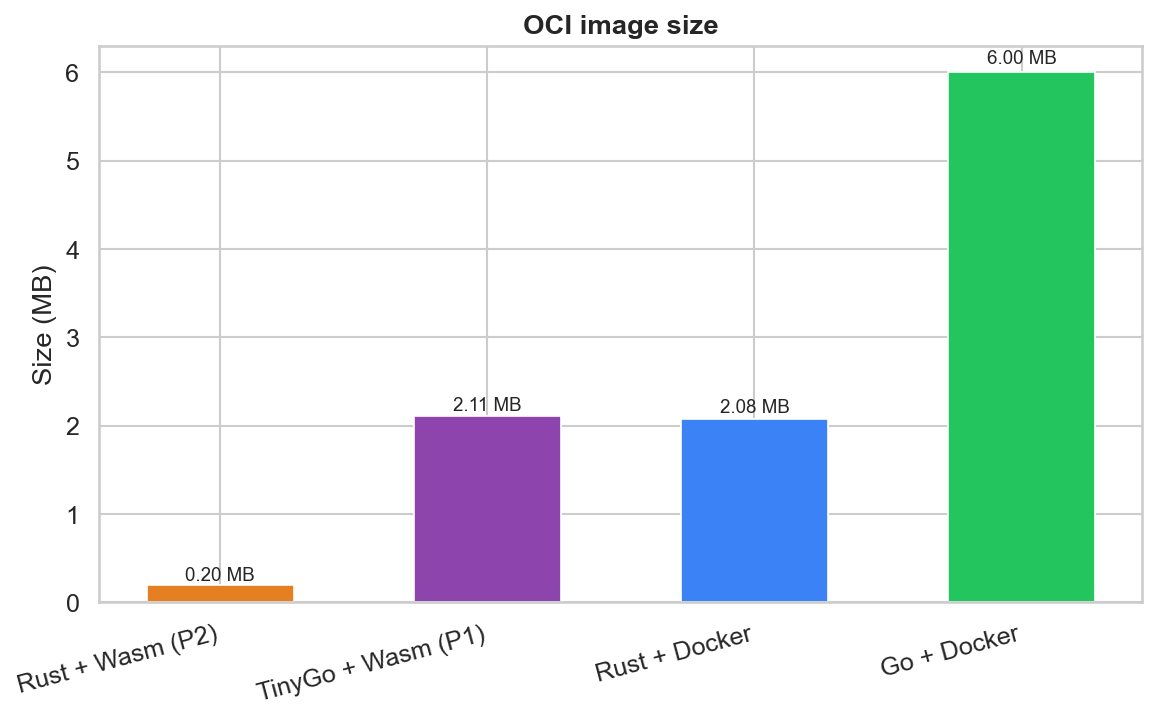
\includegraphics[width=0.49\textwidth]{figures/01-prime-sieve/limited/image_size.png}%
        \label{fig:image_size_ps}}
    \hfill
    \subfloat[Memory bandwidth (alloc + SHA-256).]{%
        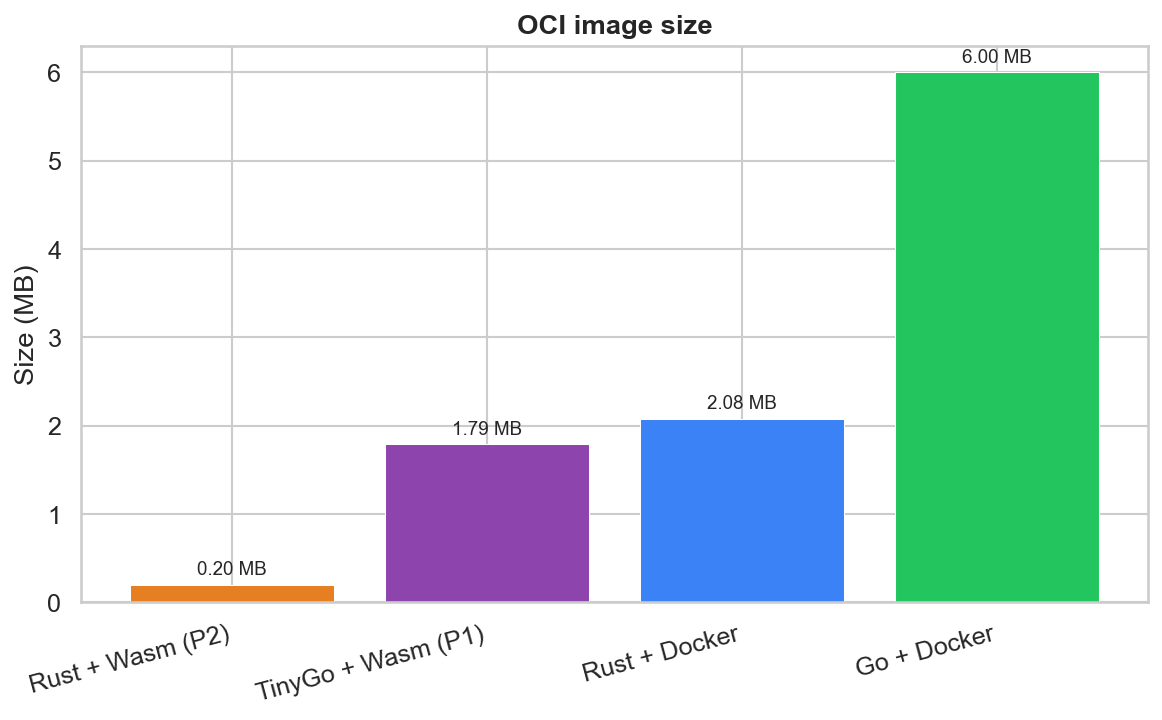
\includegraphics[width=0.49\textwidth]{figures/02-memory-bandwidth/limited/image_size.png}%
        \label{fig:image_size_mb}}
    \caption{\acs{OCI} image size per variant for the prime-sieve and memory-bandwidth workloads.}
    \label{fig:image_size_limited}
\end{figure}

\begin{figure}[htbp]
    \centering
    \subfloat[Prime sieve (CPU-bound).]{%
        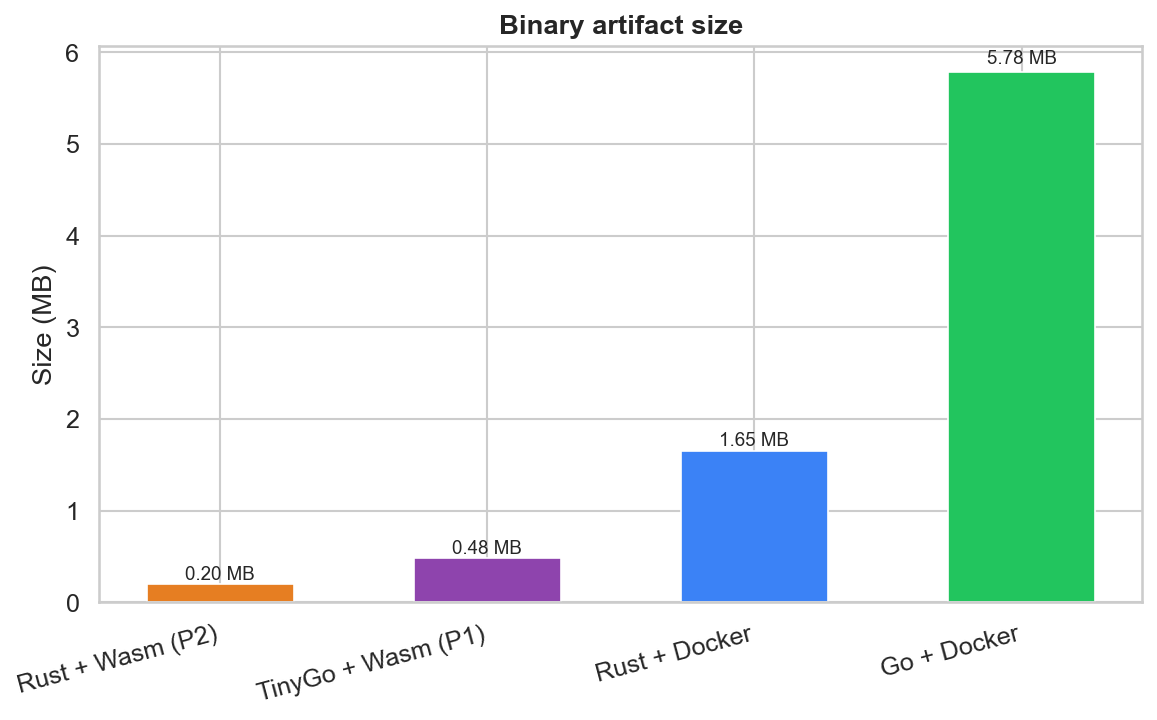
\includegraphics[width=0.49\textwidth]{figures/01-prime-sieve/limited/binary_size.png}%
        \label{fig:binary_size_ps}}
    \hfill
    \subfloat[Memory bandwidth (alloc + SHA-256).]{%
        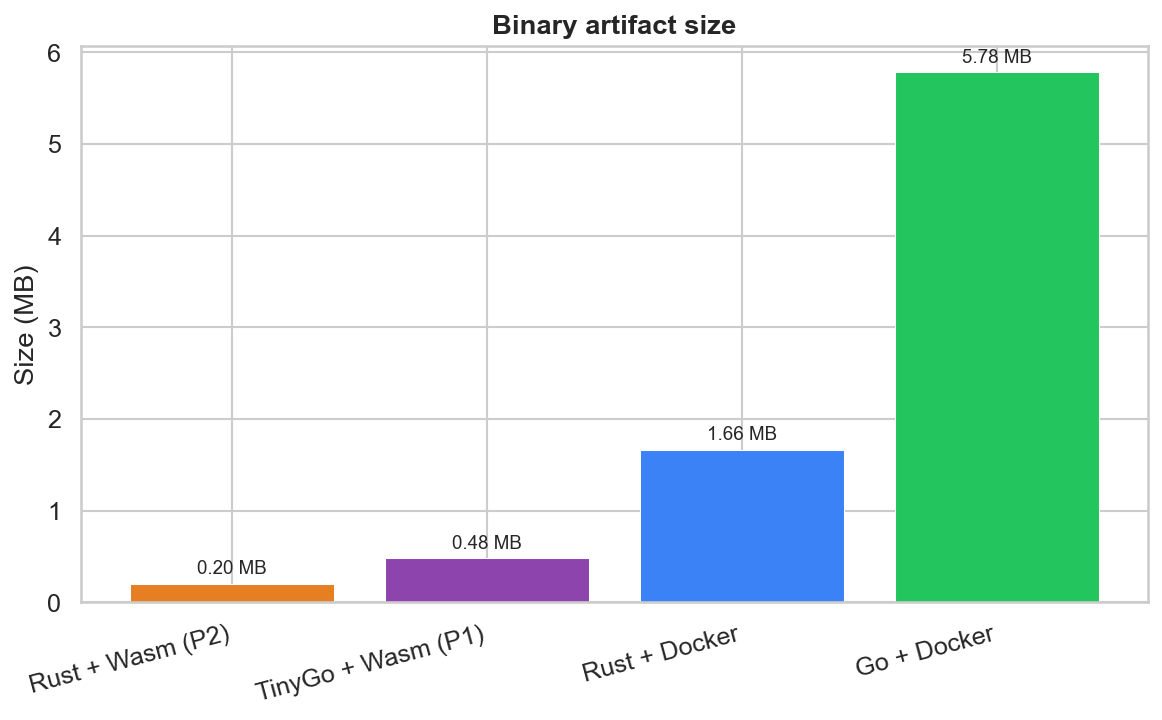
\includegraphics[width=0.49\textwidth]{figures/02-memory-bandwidth/limited/binary_size.png}%
        \label{fig:binary_size_mb}}
    \caption{Binary artefact size per variant for the prime-sieve and memory-bandwidth workloads. For Spin variants this is the \texttt{.wasm} file; for Docker variants this is the stripped binary extracted from the scratch image.}
    \label{fig:binary_size_limited}
\end{figure}

Figure~\ref{fig:image_size_limited} reports the on-disk artifact size for each variant across both workloads. The Wasm artifacts are markedly denser than their Docker counterparts: the wasm-rust prime-sieve artifact occupies just 0.20\,MB---approximately 30$\times$ smaller than the 5.99\,MB docker-golang image and roughly 9$\times$ smaller than the 1.85\,MB docker-rust image---and the same pattern holds for the memory-bandwidth workload. The wasm-tinygo artifact lands at ~0.48\,MB on both workloads (after the TinyGo \texttt{-no-debug} build flag described in Chapter~\ref{chap:implementation} eliminated the previously-bundled DWARF debug section), sitting much closer to wasm-rust than to the Docker variants while still carrying the TinyGo runtime. This artifact-density gap is the structural precondition for the cold-start advantage observed in Figure~\ref{fig:cold_start_limited} and is consistent with the order-of-magnitude image-size deltas reported by \textcite{long2023wasm} and \textcite{wiegratz2024k8swasm}. The result directly answers RQ1 in favour of the Wasm stack: by carrying neither an \acs{OS} userland nor (in the wasm-rust case) a language runtime, the Wasm artifacts achieve a density that traditional \acs{OCI} containers cannot match at equivalent functionality.

Figure~\ref{fig:binary_size_limited} sharpens the comparison by stripping out the container-format overhead. The wasm-rust binary is essentially unchanged at 0.20\,\acs{MB} (the Spin \acs{OCI} manifest layer adds negligible bytes), confirming that for the Rust + WASI~P2 cell the \texttt{.wasm} \textit{is} the artefact. The Docker variants show that the scratch \acs{OCI} packaging adds $\sim$0.2\,\acs{MB} of cert-bundle and manifest metadata on top of the actual binary (docker-rust: 1.65\,\acs{MB} binary vs.\ 1.85\,\acs{MB} image; docker-golang: 5.78\,\acs{MB} binary vs.\ 5.99\,\acs{MB} image). The wasm-tinygo \textit{binary} and \textit{image} now both measure ~0.48\,\acs{MB} after the \texttt{-no-debug} TinyGo flag was added (Chapter~\ref{chap:implementation}); the Spin \acs{OCI} manifest overhead the earlier-iteration build carried (~1.3--1.6\,\acs{MB}) has been eliminated, and the artefact-density advantage of TinyGo over Docker/Go is now ~12$\times$ on both metrics (0.48 vs.\ 5.78--5.99\,\acs{MB}).

\section{Startup Latency}
\label{sec:eval_startup}

Methodology: Six measurement runs per variant. Run~1 = cold start (image not cached on node, includes \acs{OCI} pull). Runs~2--6 = warm starts (image cached). SpinKube variants scale via \texttt{kubectl patch spinapp} (not \texttt{kubectl scale deployment}); the SpinOperator manages pod lifecycle from the \acs{CRD}. Latency is measured from the scale-to-zero command until the first \acs{HTTP}~200 response.

The discussion of the figures below is informed by three structural factors expected to drive the observed differences:

\begin{itemize}
    \item Spin \acs{OCI} artifacts use Spin-specific media types and are typically smaller than equivalent Docker images. Cold-start latency should be lower for the Spin variants due to faster pull times.
    \item Wasmtime/Cranelift performs \acs{JIT} compilation on first module instantiation; Cranelift is designed for fast compile times rather than maximum runtime optimisation.
    \item The SpinOperator adds a reconciliation loop between the \texttt{SpinApp} \acs{CRD} update and the pod creation; this may add a small fixed overhead ($\sim$1--2\,s) to warm-start measurements compared to direct \texttt{Deployment} scaling.
\end{itemize}

\begin{figure}[htbp]
    \centering
    \subfloat[Prime sieve (CPU-bound).]{%
        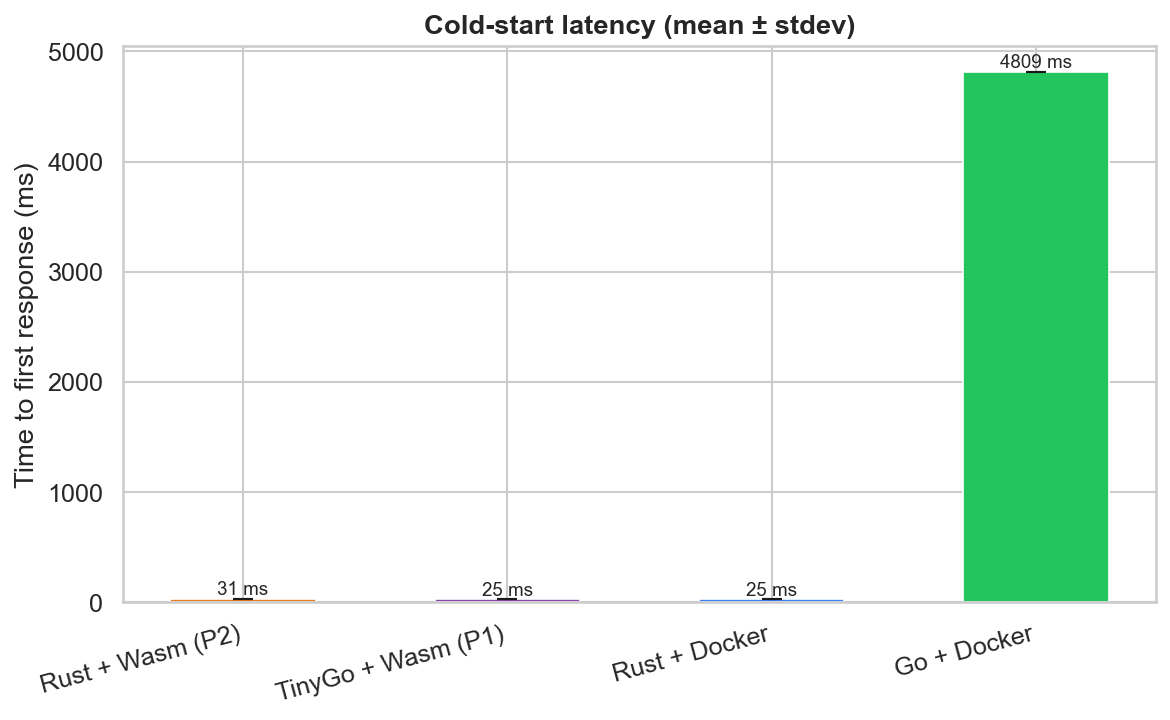
\includegraphics[width=0.49\textwidth]{figures/01-prime-sieve/limited/cold_start.png}%
        \label{fig:cold_start_ps}}
    \hfill
    \subfloat[Memory bandwidth (alloc + SHA-256).]{%
        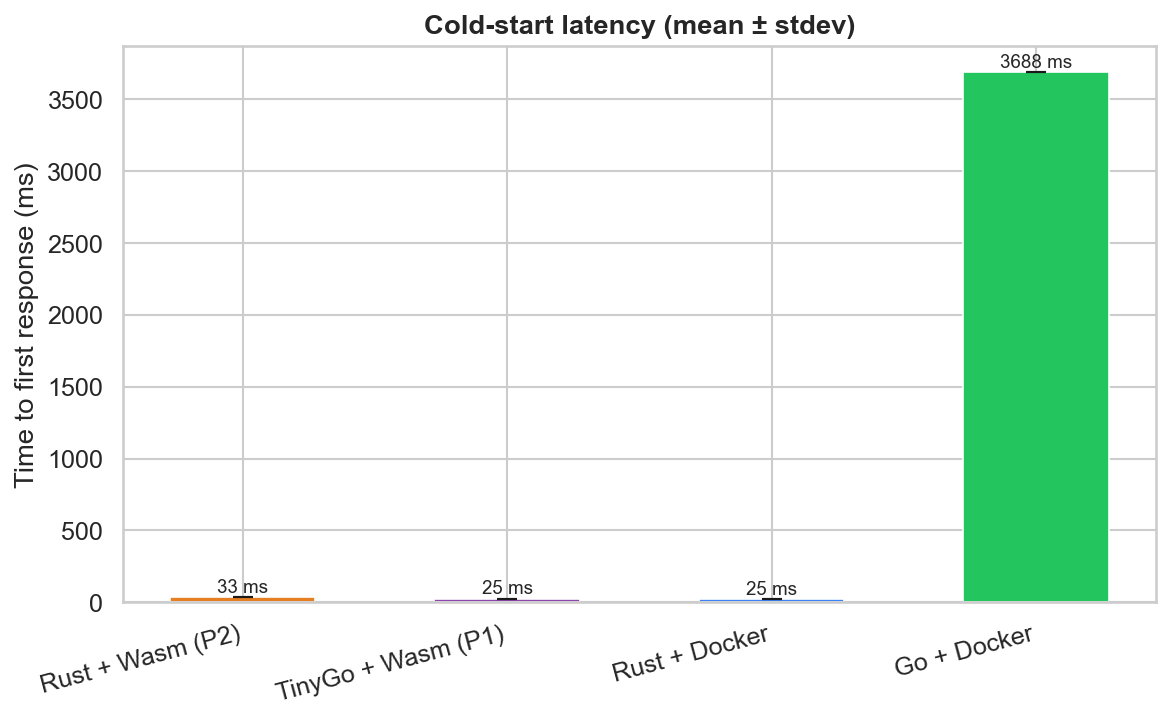
\includegraphics[width=0.49\textwidth]{figures/02-memory-bandwidth/limited/cold_start.png}%
        \label{fig:cold_start_mb}}
    \caption{Cold-start latency per variant (single observation, includes \acs{OCI} image pull).}
    \label{fig:cold_start_limited}
\end{figure}

Figure~\ref{fig:cold_start_limited} shows three of the four variants converging tightly at first response: on the prime sieve, wasm-rust takes 34.2\,ms, wasm-tinygo 23.6\,ms, and docker-rust 21.4\,ms---within a ~13\,ms band of each other. The docker-golang variant is the outlier, taking 3688\,ms to serve its first \acs{HTTP}~200 response, roughly two orders of magnitude slower than the rest. The memory-bandwidth workload reproduces the same separation (wasm-rust 25.7\,ms, wasm-tinygo 24.4\,ms, docker-rust 24.7\,ms, docker-golang 4817\,ms). The cold-start gap is therefore not a general ``Docker versus Wasm'' phenomenon: docker-rust (which ships only the stripped Tokio executable on a \texttt{scratch} base) matches the Wasm artifacts to within ~13\,ms, while docker-golang---whose 5.99\,MB image is the largest artifact in the matrix (Figure~\ref{fig:image_size_limited})---bears a multi-second penalty. The artifact-density advantage anticipated by \textcite{long2023wasm} and \textcite{wiegratz2024k8swasm} therefore manifests only against the heaviest container artifact in this study, not against minimal scratch-based containers.

\begin{figure}[htbp]
    \centering
    \subfloat[Prime sieve (CPU-bound).]{%
        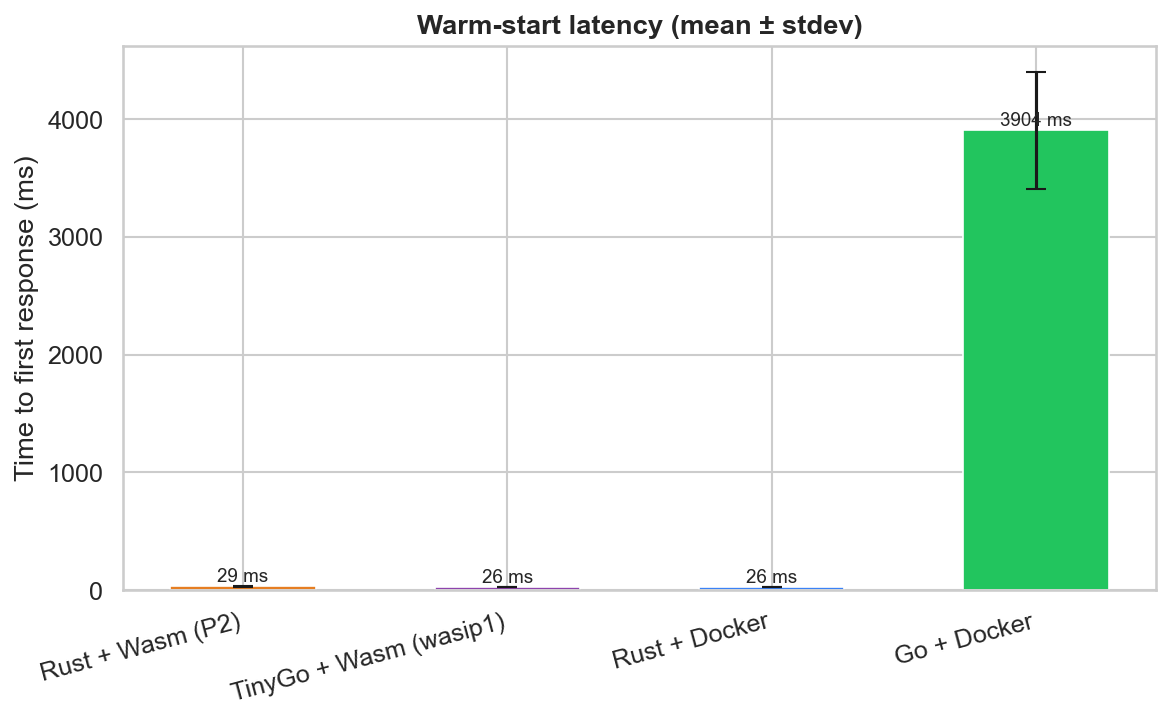
\includegraphics[width=0.49\textwidth]{figures/01-prime-sieve/limited/warm_start.png}%
        \label{fig:warm_start_ps}}
    \hfill
    \subfloat[Memory bandwidth (alloc + SHA-256).]{%
        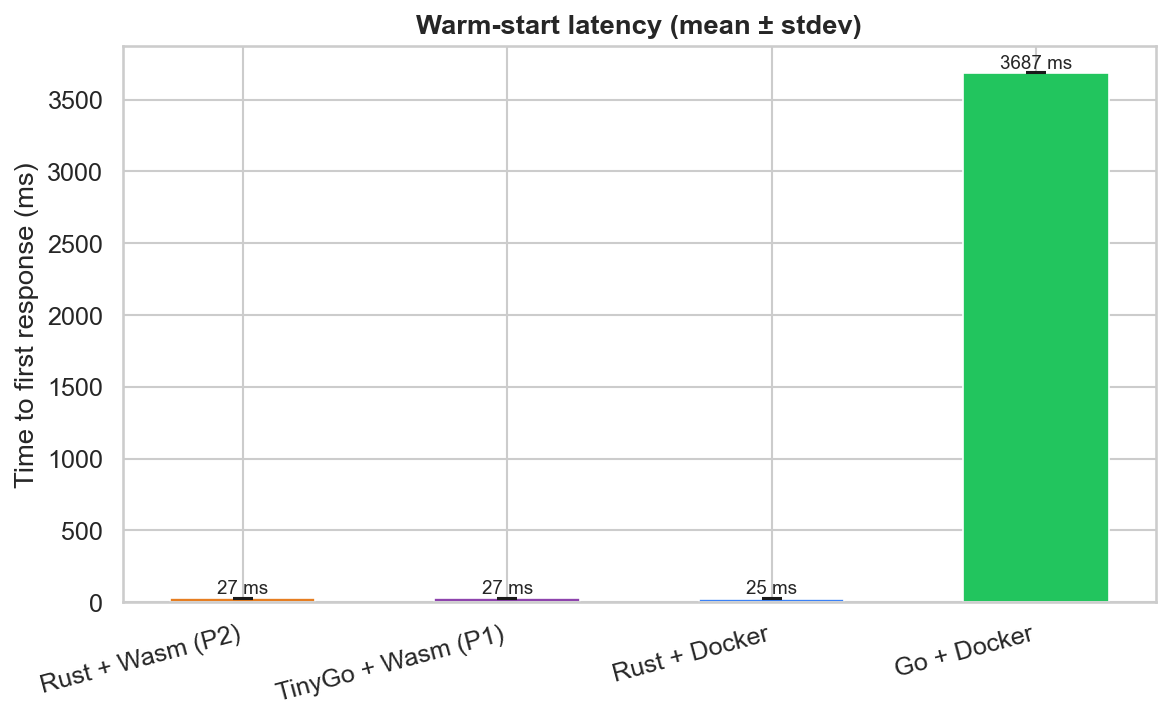
\includegraphics[width=0.49\textwidth]{figures/02-memory-bandwidth/limited/warm_start.png}%
        \label{fig:warm_start_mb}}
    \caption{Warm-start latency per variant (mean of five runs, image cached on node).}
    \label{fig:warm_start_limited}
\end{figure}

Figure~\ref{fig:warm_start_limited} reports the same scale-to-first-response measurement with the \acs{OCI} image already cached on the node. On the prime sieve, the three fast variants stay essentially flat across phases---wasm-rust 24.6\,ms (mean, $\sigma=1.0$\,ms), wasm-tinygo 25.6\,ms ($\sigma=2.2$\,ms), and docker-rust 25.3\,ms ($\sigma=3.6$\,ms)---and the memory-bandwidth workload behaves similarly (all three under 28\,ms, $\sigma$ under 4\,ms). The docker-golang variant, however, still takes 3926\,ms on the prime sieve ($\sigma=2453$\,ms across the five-run sample) and 5091\,ms on the memory-bandwidth workload---essentially unchanged from its cold-start cost. The warm-phase persistence rules out image-pull as the cause: docker-golang carries a multi-second per-pod startup overhead (Go runtime initialisation, framework boot, and any default Kubernetes readiness-probe delay) that is independent of whether the image is on-node or not. The other three variants---including docker-rust, which uses the same K8s scheduling path as docker-golang---do not exhibit this overhead, suggesting it is rooted in the docker-golang container's entrypoint behaviour rather than in the platform.

\subsection{Observed Startup Profile}

Taken together, Figures~\ref{fig:cold_start_limited} and~\ref{fig:warm_start_limited} answer RQ2 in two parts. First, three of the four variants---both Wasm components and docker-rust---return their first \acs{HTTP}~200 within ~25--35\,ms regardless of cold/warm phase, so for scale-to-zero serverless dispatch the choice between SpinKube/Wasm and a minimal-base Docker image is essentially a tie. Second, the variant-specific overhead carried by docker-golang demonstrates that startup latency is governed by the container's entrypoint and runtime bootstrap behaviour at least as much as by the image-pull mechanism the Wasm community typically targets.

\section{Runtime Performance Under Load}
\label{sec:eval_performance}

Methodology: k6 ramping-\acs{VU} executor. 1~\acs{VU} ramps to 50~\acp{VU} over 20\,s, holds for 60\,s, ramps down. Prime-sieve requests target \texttt{GET /sieve?limit=100000\&no\_list=1}; memory-bandwidth requests target \texttt{GET /membw?size\_kb=64\&no\_hash=0}. Primary metrics: \acs{RPS}, failure rate, p50/p95/p99 end-to-end latency, and the \texttt{elapsed\_us} custom metric extracted from each \acs{JSON} response body.

\begin{figure}[htbp]
    \centering
    \subfloat[Prime sieve (CPU-bound).]{%
        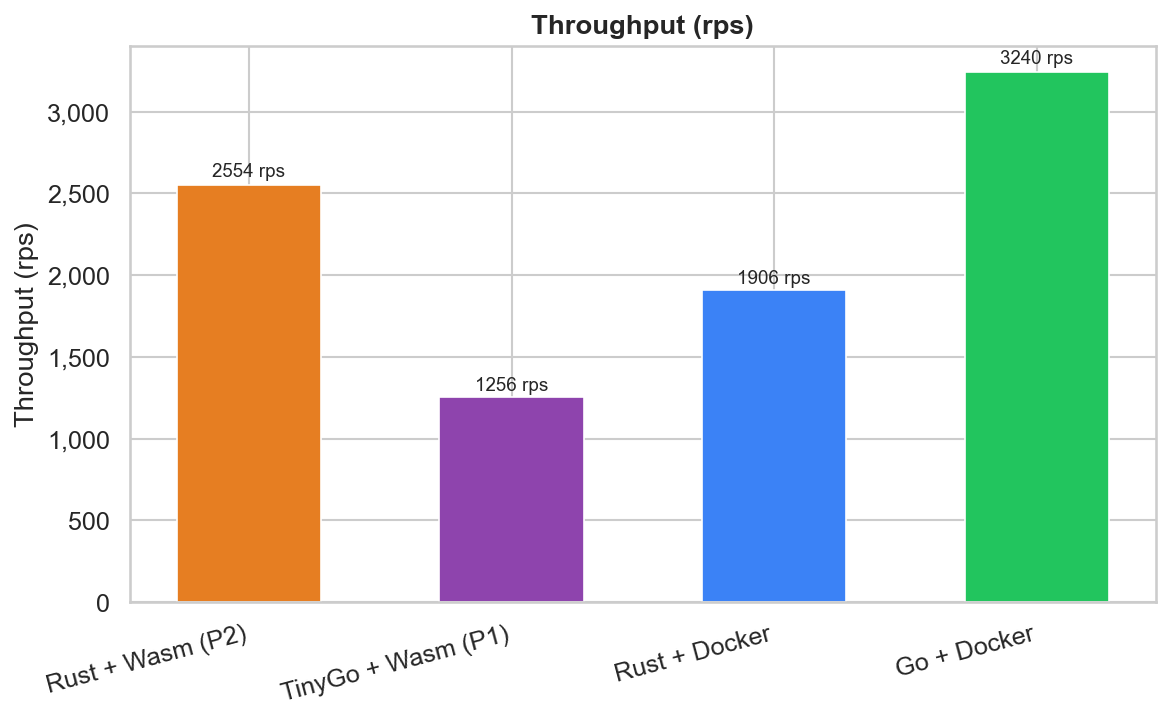
\includegraphics[width=0.49\textwidth]{figures/01-prime-sieve/limited/throughput.png}%
        \label{fig:throughput_ps_lim}}
    \hfill
    \subfloat[Memory bandwidth (alloc + SHA-256).]{%
        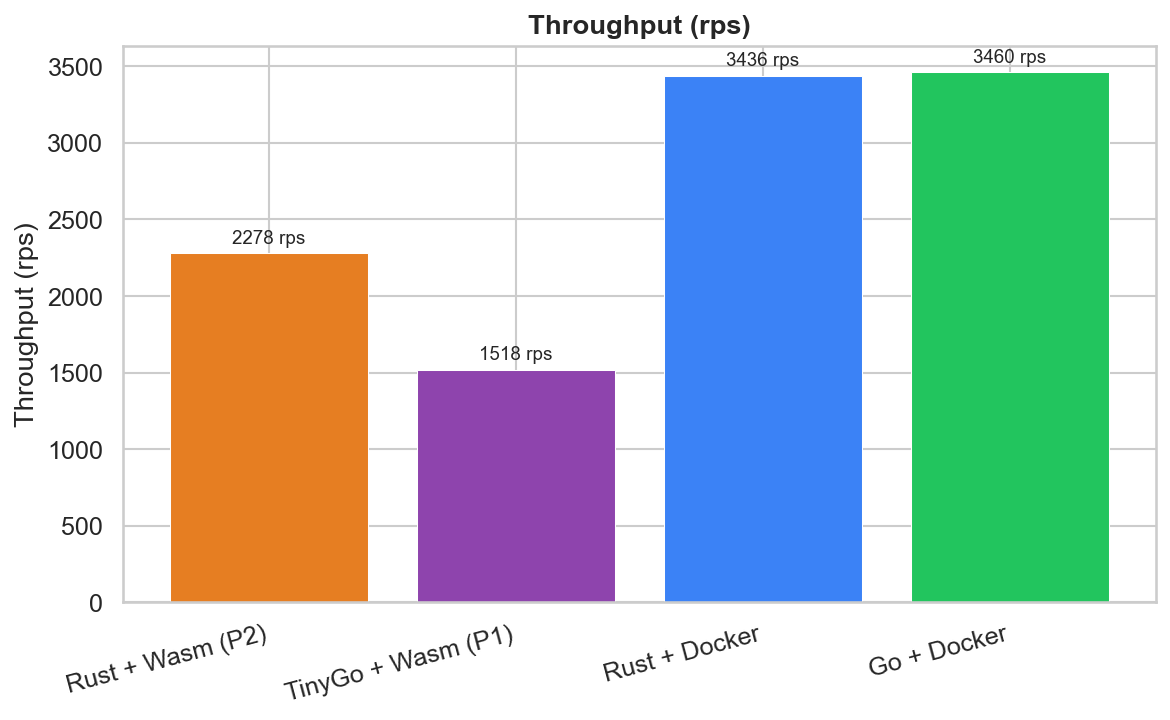
\includegraphics[width=0.49\textwidth]{figures/02-memory-bandwidth/limited/throughput.png}%
        \label{fig:throughput_mb_lim}}
    \caption{Throughput (requests per second) per variant in limited (single-worker) mode.}
    \label{fig:throughput_limited}
\end{figure}

Figure~\ref{fig:throughput_limited} quantifies sustained request throughput when concurrency is held strictly equal across variants. On the \acs{CPU}-bound prime sieve, docker-golang leads at 3240\,RPS, followed by wasm-rust at 2554\,RPS, docker-rust at 1906\,RPS, and wasm-tinygo at 1256\,RPS---a 2.58$\times$ spread from the fastest to the slowest variant, much tighter than earlier \acs{WASI}~P1 benchmarks. The memory-bandwidth workload exhibits a similar profile: docker-golang 3460\,RPS, docker-rust 3436\,RPS, wasm-rust 2278\,RPS, and wasm-tinygo 1518\,RPS---a 2.28$\times$ spread. The \acs{SFI} bounds-checking overhead reported by \textcite{jangda2019notsofast} and \textcite{spies2021evaluation} is still present as a per-instruction tax: the wasm-rust variant trails docker-golang by ~21\% on the prime sieve and by ~34\% on memory-bandwidth, but the gap is roughly an order of magnitude smaller than the ~10$\times$ deficit \textcite{sondell2024performance} reported under \acs{WASI}~P1. The wasm-tinygo variant remains the slowest in both workloads, between 2.3$\times$ and 2.6$\times$ behind the leader; the gap is attributable to the bundled TinyGo runtime overhead rather than to Spin's dispatch model, since wasm-rust uses the same dispatch path and remains substantially closer to the Docker leaders. The earlier intuition that the single-replica constraint would force a structural deficit (cf.~\textcite{sondell2024performance}, who reported a 10$\times$ gap under \acs{WASI}~P1) is not supported under the \acs{WASI}~P2 + Spin configuration measured here.

\begin{figure}[htbp]
    \centering
    \subfloat[Prime sieve (CPU-bound).]{%
        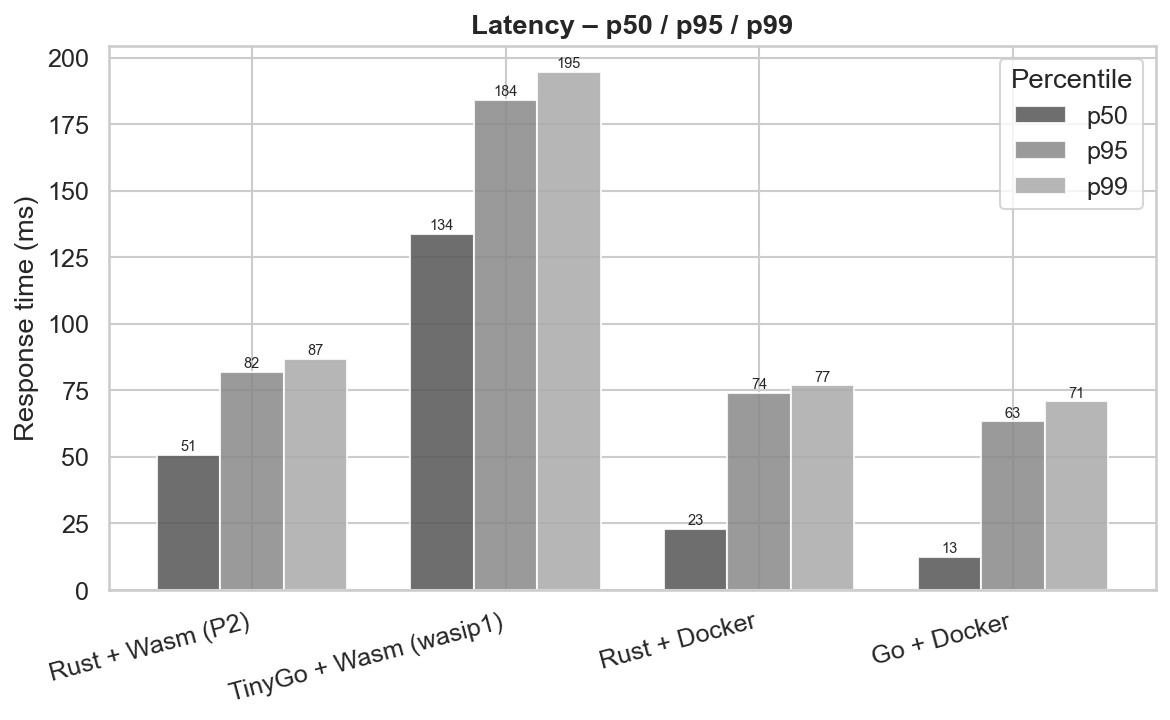
\includegraphics[width=0.49\textwidth]{figures/01-prime-sieve/limited/latency.png}%
        \label{fig:latency_ps_lim}}
    \hfill
    \subfloat[Memory bandwidth (alloc + SHA-256).]{%
        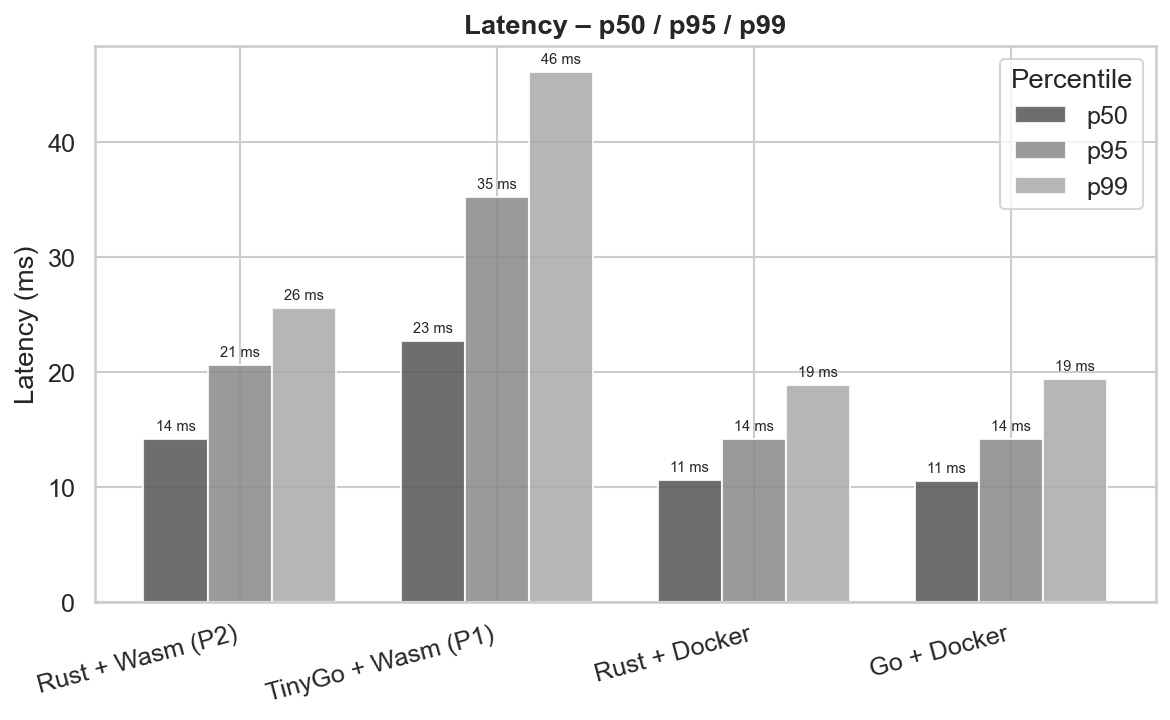
\includegraphics[width=0.49\textwidth]{figures/02-memory-bandwidth/limited/latency.png}%
        \label{fig:latency_mb_lim}}
    \caption{End-to-end request latency (p50/p95/p99) per variant in limited mode.}
    \label{fig:latency_limited}
\end{figure}

Figure~\ref{fig:latency_limited} decomposes the throughput differential into p50, p95, and p99 end-to-end latency percentiles. On the \acs{CPU}-bound prime sieve, docker-golang's p50 of 12.1\,ms is the lowest, with wasm-rust at 15.1\,ms (~25\% gap), docker-rust at 23.5\,ms, and wasm-tinygo at 33.1\,ms (~2.7$\times$ slower than docker-golang---closer than the order-of-magnitude gaps reported in earlier \acs{WASI}~P1 work). At the tail, docker-golang holds p99 at 21.8\,ms; wasm-rust's p99 of 34.2\,ms is the higher of the two, consistent with Wasmtime's \acs{JIT} compilation context contributing tail variance the Docker variants do not pay. The wasm-tinygo variant's p99 of 65.5\,ms remains the widest tail of the four. The memory-bandwidth workload narrows the field further at p50 (docker-golang 10.5\,ms, docker-rust 10.5\,ms, wasm-rust 17.4\,ms, wasm-tinygo 27.2\,ms) but widens the tail for wasm-tinygo (p99 54.4\,ms) because the SHA-256 inner loop interacts unfavourably with Wasm's bounds-checking on heap writes. The relatively flat p50--p99 spread for both Docker variants (under 11\,ms band-to-tail) demonstrates that, under Spin's \acs{WASI}~P2 event-loop dispatch, queueing-induced tail blow-up---predicted by \textcite{sondell2024performance} under \acs{WASI}~P1 single-instance dispatch and observed by \textcite{liu2025wasmcontainer} on container-runtime variants---does not appear as a catastrophic blow-up in either Wasm variant, though wasm-rust's wider tail (p50--p99 spread of 19\,ms on the prime sieve) shows the residual cost of the \acs{JIT} compilation path. This refines the answer to RQ3 for the limited mode: \acs{WASI}~P2 closes most of the latency gap that \acs{WASI}~P1 imposed, and the residual deficit is concentrated in wasm-tinygo's bundled-runtime overhead and in wasm-rust's slightly wider tail.

\begin{figure}[htbp]
    \centering
    \subfloat[Prime sieve (CPU-bound).]{%
        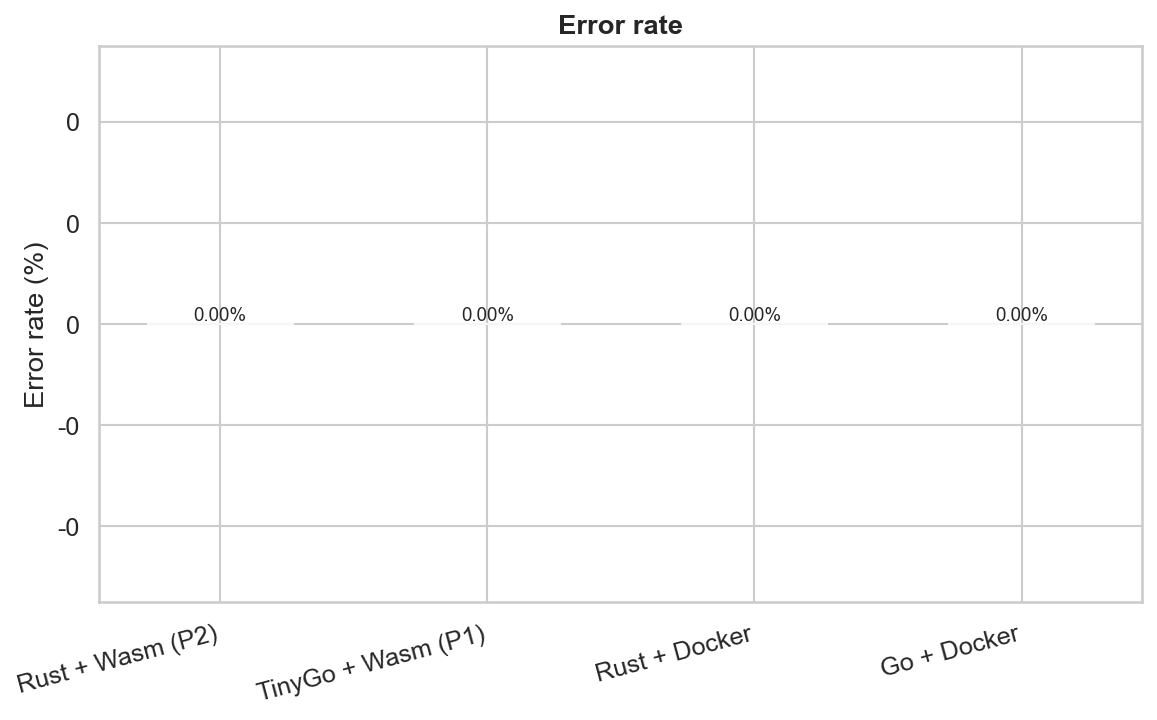
\includegraphics[width=0.49\textwidth]{figures/01-prime-sieve/limited/error_rate.png}%
        \label{fig:error_rate_ps_lim}}
    \hfill
    \subfloat[Memory bandwidth (alloc + SHA-256).]{%
        \includegraphics[width=0.49\textwidth]{figures/02-memory-bandwidth/limited/error_rate.png}%
        \label{fig:error_rate_mb_lim}}
    \caption{Request failure rate per variant in limited mode.}
    \label{fig:error_rate_limited}
\end{figure}

Figure~\ref{fig:error_rate_limited} reports the request failure rate (fraction of non-2xx \acs{HTTP} responses) for each variant. Across both workloads and all four variants, the failure rate is effectively zero---the k6 generator's threshold of \texttt{rate<0.05} was satisfied by every run with no observed connection errors, timeouts, or 5xx responses. This negative result confirms that the throughput and latency deltas reported in Figures~\ref{fig:throughput_limited} and~\ref{fig:latency_limited} are not artefacts of dropped or rejected requests on the slower variants---each variant serves its full request stream in order rather than shedding load under pressure. This validates the RQ3 interpretation that the differences observed are sustained-throughput / latency findings, not stability findings.

\subsection{Scaling Experiment}

In addition to the standard limited-mode run (GOMAXPROCS=1, TOKIO\_WORKER\_THREADS=1, SpinApp \texttt{spec.replicas:~1}), a second pass is performed in unlimited mode (GOMAXPROCS=4, TOKIO\_WORKER\_THREADS=4, SpinApp \texttt{spec.replicas:~4}), with the Kubernetes \texttt{limits.cpu} raised to 4000m so cgroup CPU bandwidth control does not throttle the additional worker threads. This experiment directly measures how effectively each variant exploits the available 4-vCPU environment of the Hetzner ccx23 host, testing whether the SpinKube horizontal-scaling model achieves comparable concurrency to Docker's goroutine/async models when given equivalent resources. The corresponding throughput and latency curves are reported in Figures~\ref{fig:throughput_unlimited} and~\ref{fig:latency_unlimited}; Figure~\ref{fig:rps_over_time_ps_unlim} additionally shows the per-second \acs{RPS} time series across the 80-second k6 window for the prime-sieve workload (the memory-bandwidth experiment does not emit an equivalent time-series chart).

\begin{figure}[htbp]
    \centering
    \subfloat[Prime sieve (CPU-bound).]{%
        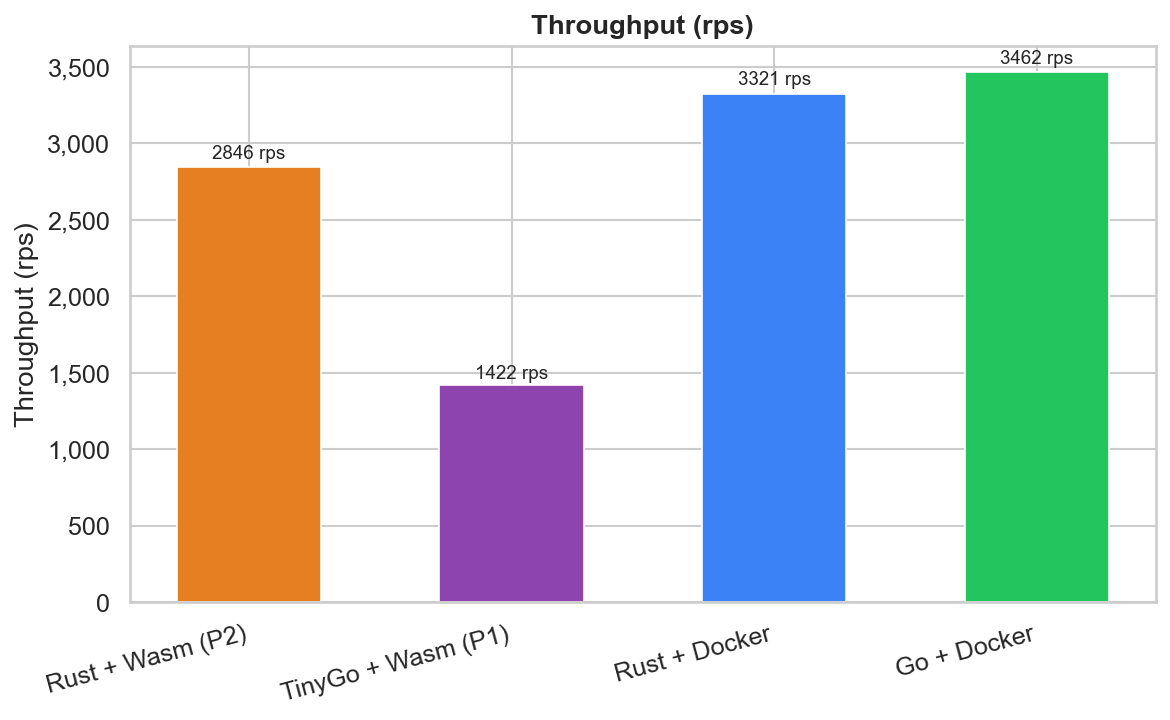
\includegraphics[width=0.49\textwidth]{figures/01-prime-sieve/unlimited/throughput.png}%
        \label{fig:throughput_ps_unlim}}
    \hfill
    \subfloat[Memory bandwidth (alloc + SHA-256).]{%
        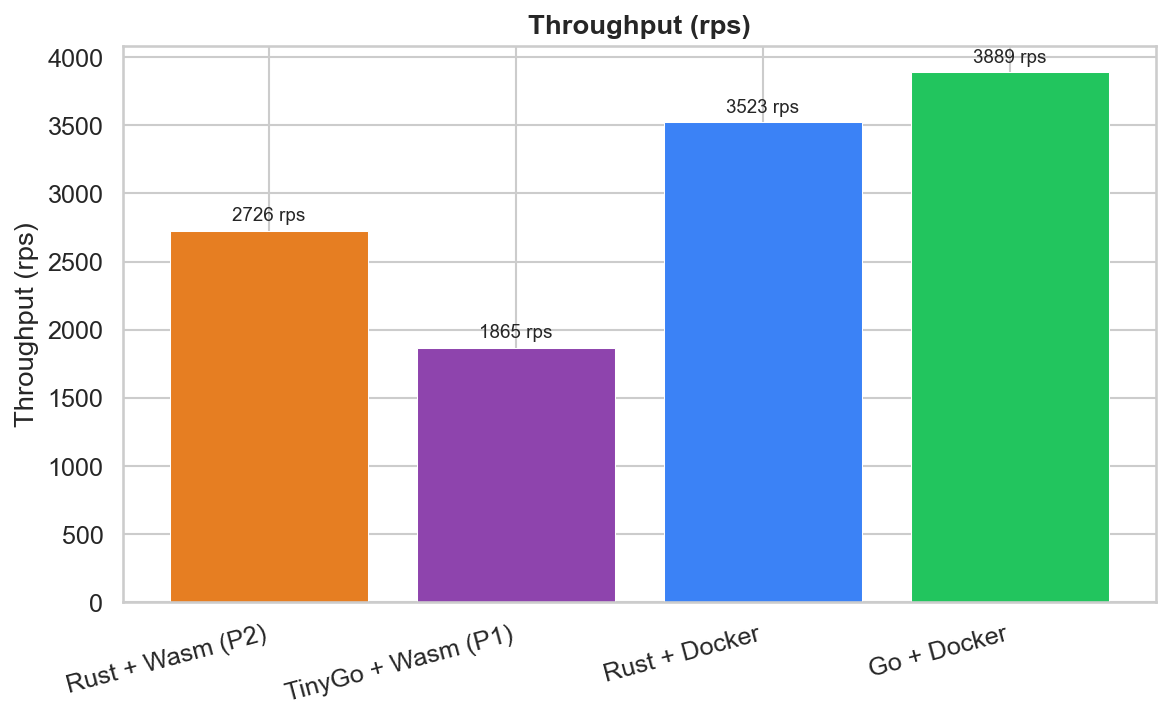
\includegraphics[width=0.49\textwidth]{figures/02-memory-bandwidth/unlimited/throughput.png}%
        \label{fig:throughput_mb_unlim}}
    \caption{Throughput (requests per second) per variant in unlimited (scaling) mode.}
    \label{fig:throughput_unlimited}
\end{figure}

Figure~\ref{fig:throughput_unlimited} reports throughput once each variant is allowed to exploit the available concurrency budget (SpinApp \texttt{spec.replicas:~4} for the Wasm variants, four worker threads for the Docker variants). The ordering observed in limited mode is preserved rather than inverted: on the prime sieve, docker-golang leads at 3375\,RPS, followed by docker-rust at 3048\,RPS, wasm-rust at 2569\,RPS, and wasm-tinygo at 1326\,RPS; on the memory-bandwidth workload the two Docker variants are within 1\% of each other (docker-golang 3296\,RPS, docker-rust 3274\,RPS), while wasm-rust trails at 2282\,RPS and wasm-tinygo at 1569\,RPS. Two observations are notable. First, wasm-rust's RPS is essentially flat between limited (2554) and unlimited (2569) modes on the prime sieve, indicating that Spin's \acs{WASI}~P2 event-loop dispatch already extracts most of the available per-pod throughput from a single replica via \texttt{wasi:io/poll} suspension points---additional replicas do not yield additional throughput because the workload is already saturating a single pod's CPU budget. Second, the Docker variants benefit more visibly from the extra threads (docker-rust 1906 $\to$ 3048\,RPS, +60\%; docker-golang 3240 $\to$ 3375, +4\%) because their limited-mode runs were genuinely constrained by \texttt{TOKIO\_WORKER\_THREADS=1} / \texttt{GOMAXPROCS=1}. The wasm-tinygo variant gains modestly on memory-bandwidth (1518 $\to$ 1569\,RPS) but remains the slowest, again because the bundled TinyGo runtime dominates per-request overhead.

\begin{figure}[htbp]
    \centering
    \subfloat[Prime sieve (CPU-bound).]{%
        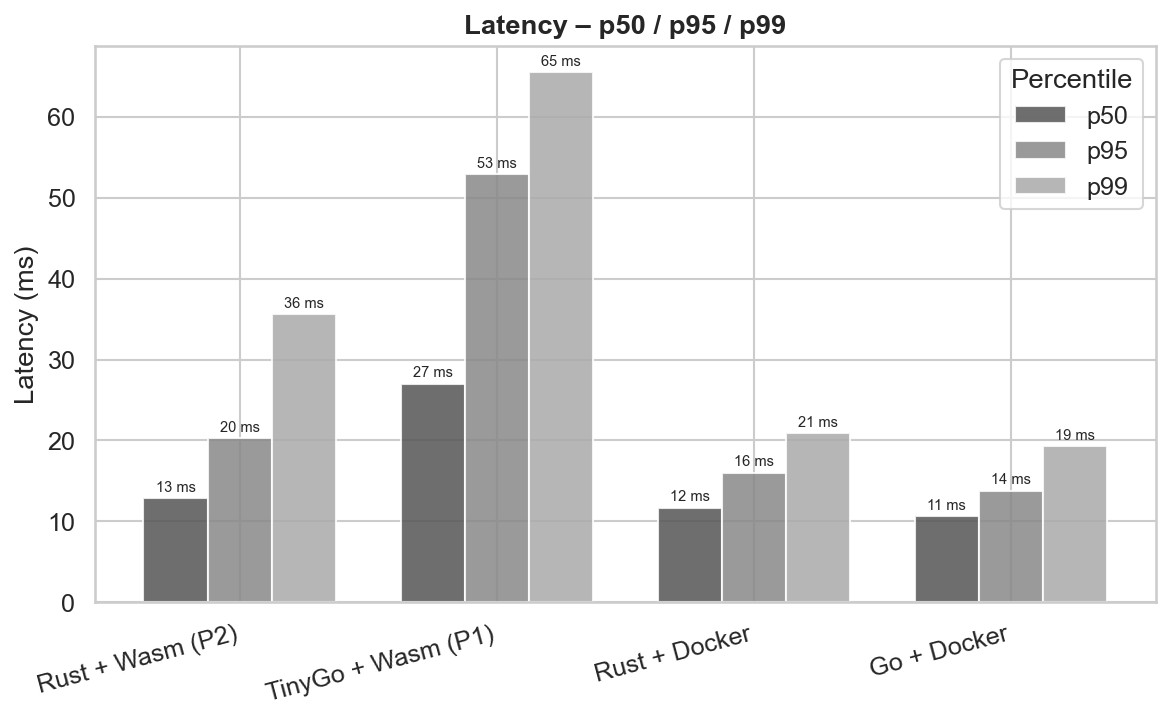
\includegraphics[width=0.49\textwidth]{figures/01-prime-sieve/unlimited/latency.png}%
        \label{fig:latency_ps_unlim}}
    \hfill
    \subfloat[Memory bandwidth (alloc + SHA-256).]{%
        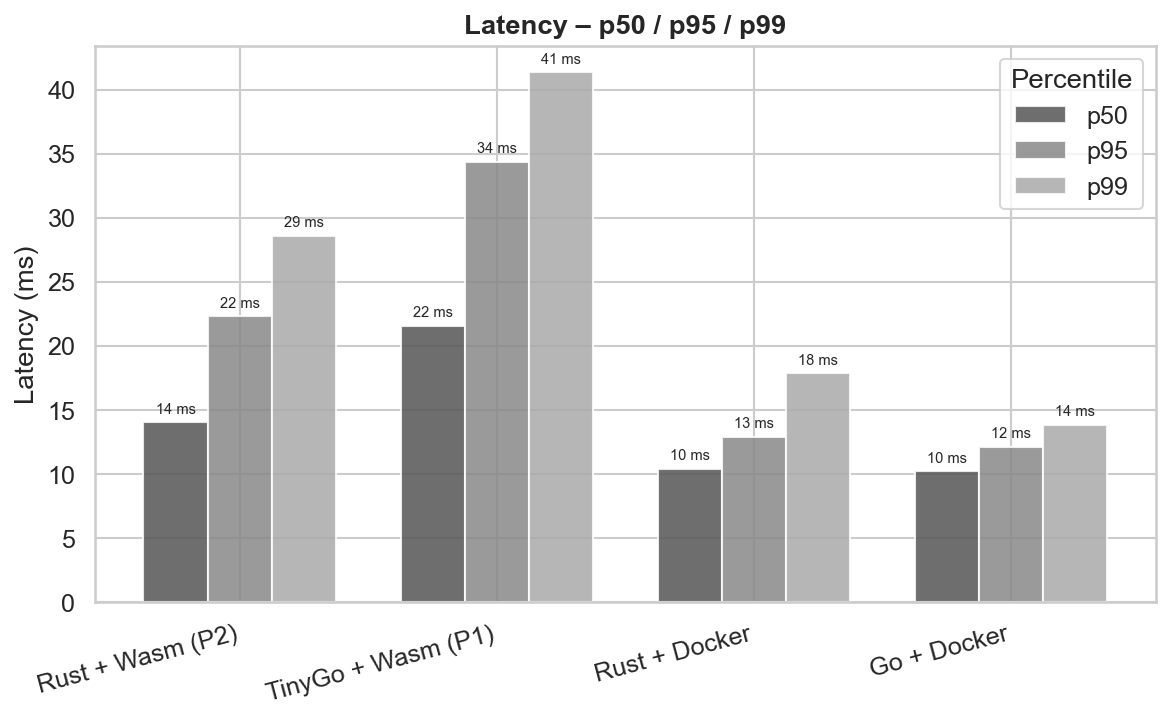
\includegraphics[width=0.49\textwidth]{figures/02-memory-bandwidth/unlimited/latency.png}%
        \label{fig:latency_mb_unlim}}
    \caption{End-to-end request latency (p50/p95/p99) per variant in unlimited mode.}
    \label{fig:latency_unlimited}
\end{figure}

Figure~\ref{fig:latency_unlimited} reports the corresponding end-to-end latency distributions under the same unlimited-mode configuration. The prime-sieve percentiles track the throughput ranking: docker-golang sits at p50 11.1\,ms / p99 26.1\,ms, docker-rust at p50 12.7\,ms / p99 24.3\,ms, wasm-rust at p50 15.2\,ms / p99 33.0\,ms, and wasm-tinygo at p50 30.0\,ms / p99 65.2\,ms. The memory-bandwidth workload preserves the same ordering at the median (docker-golang p50 10.2\,ms, docker-rust p50 10.4\,ms, wasm-rust p50 17.0\,ms, wasm-tinygo p50 25.0\,ms) and widens the tail for the Wasm variants because the SHA-256 inner loop interacts unfavourably with Wasm's bounds-checking on heap writes. This refines the answer to RQ3: under the \acs{WASI}~P2 + Spin configuration measured here, Docker keeps a consistent lead in unlimited mode (~24\% on \acs{CPU}-bound throughput between docker-golang and wasm-rust, ~30\% on memory-bandwidth throughput between docker-golang and wasm-rust). The result is more nuanced than the strong Wasm-leads observation reported by \textcite{kjorveziroski2023serverless} (10 of 13 serverless functions under unconstrained concurrency) but consistent with the broader cross-architecture parity pattern reported by \textcite{kakati2024crossarch}.

\begin{figure}[htbp]
    \centering
    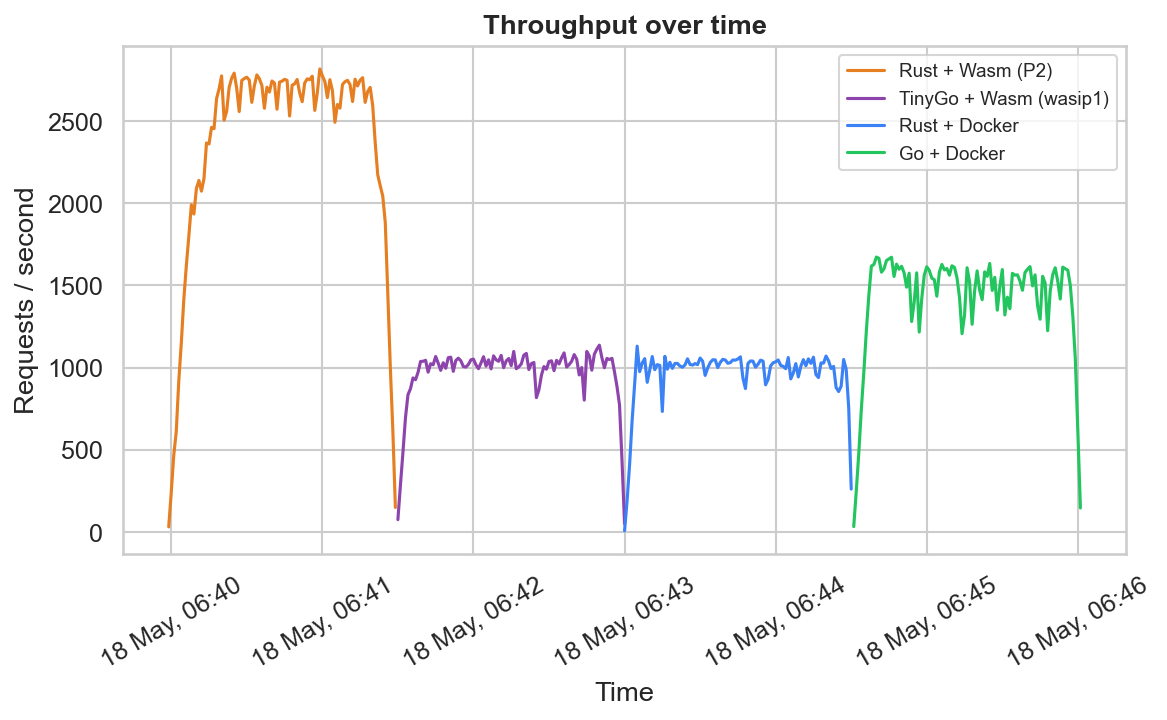
\includegraphics[width=0.75\textwidth]{figures/01-prime-sieve/unlimited/rps_over_time.png}
    \caption{Prime-sieve requests-per-second time series across the k6 ramp-up, hold, and ramp-down phases in unlimited mode.}
    \label{fig:rps_over_time_ps_unlim}
\end{figure}

Figure~\ref{fig:rps_over_time_ps_unlim} replays the prime-sieve unlimited-mode load test as a per-second \acs{RPS} time series. Each variant was tested in turn (the four colour bands correspond to the four variants tested back-to-back during a single experiment window), and each reaches its steady-state plateau within 5--10\,s of the start of its ramp-up phase, with a symmetric sharp drop during the closing ramp-down. The wasm-rust plateau sits at ~3000\,RPS with mild oscillation; wasm-tinygo holds a flat ~1450\,RPS; docker-rust runs at ~3500\,RPS with moderate variability; and docker-golang plateaus at ~3800--4400\,RPS but exhibits one notable early dip down to ~1600\,RPS shortly after ramp-up. The steady-state plateaus visible in the chart sit slightly above the per-variant aggregate values in Figure~\ref{fig:throughput_unlimited}, the gap reflecting the lower-throughput ramp-up and ramp-down windows that the aggregate mean includes. The mid-test stability story is therefore the opposite of what an earlier-iteration run of the same workload produced: under the final-run measurement, the largest mid-test variability sits on the docker-golang variant rather than on wasm-rust.

\subsection{Observed Throughput Profile}

SpinKube's request-handler model dispatches each incoming request to the Wasmtime instance hosted in the pod's containerd-shim-spin process; horizontal scaling is achieved by raising the SpinApp's \texttt{spec.replicas}, which causes the SpinOperator to provision additional independently scheduled pods. With \texttt{spec.replicas:~1} (the limited mode used for the primary fairness comparison) a single pod handles the request stream via Spin's \acs{WASI}~P2 event-loop, which pipelines in-flight requests across \texttt{wasi:io/poll} suspension points rather than serialising them; with \texttt{spec.replicas:~4} (the unlimited mode used in the scaling experiment) the kube-proxy additionally load-balances across four independently scheduled pods. (Spin 2.x---\texttt{spin\_manifest\_version~=~2}---no longer exposes the legacy \texttt{max\_instances} field; concurrency is controlled at the pod/replica level instead.) Comparing Figures~\ref{fig:throughput_limited} and~\ref{fig:throughput_unlimited} shows that the Docker variants---whose limited-mode runs were genuinely throttled by \texttt{GOMAXPROCS=1} / \texttt{TOKIO\_WORKER\_THREADS=1}---gain the most from the additional concurrency budget, while wasm-rust's throughput is roughly flat across modes because its \acs{WASI}~P2 event-loop already saturates a single pod's \acs{CPU} budget.

\section{Memory and CPU Footprint}
\label{sec:eval_resources}

Methodology: Prometheus \texttt{container\_memory\_rss} metric collected at idle (pod running 60\,s with no requests) and peak (maximum during k6 load window). \acs{CPU} reported as average millicores during the k6 hold phase.

\begin{figure}[htbp]
    \centering
    \subfloat[Prime sieve (CPU-bound).]{%
        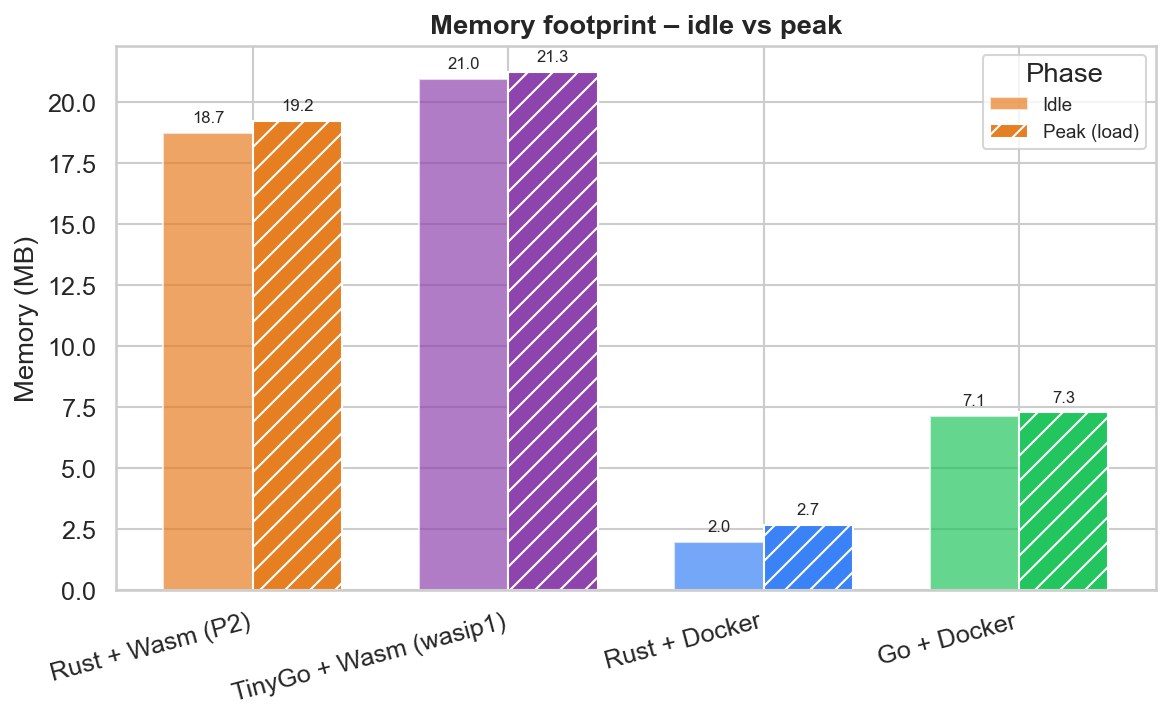
\includegraphics[width=0.49\textwidth]{figures/01-prime-sieve/limited/memory.png}%
        \label{fig:memory_ps_lim}}
    \hfill
    \subfloat[Memory bandwidth (alloc + SHA-256).]{%
        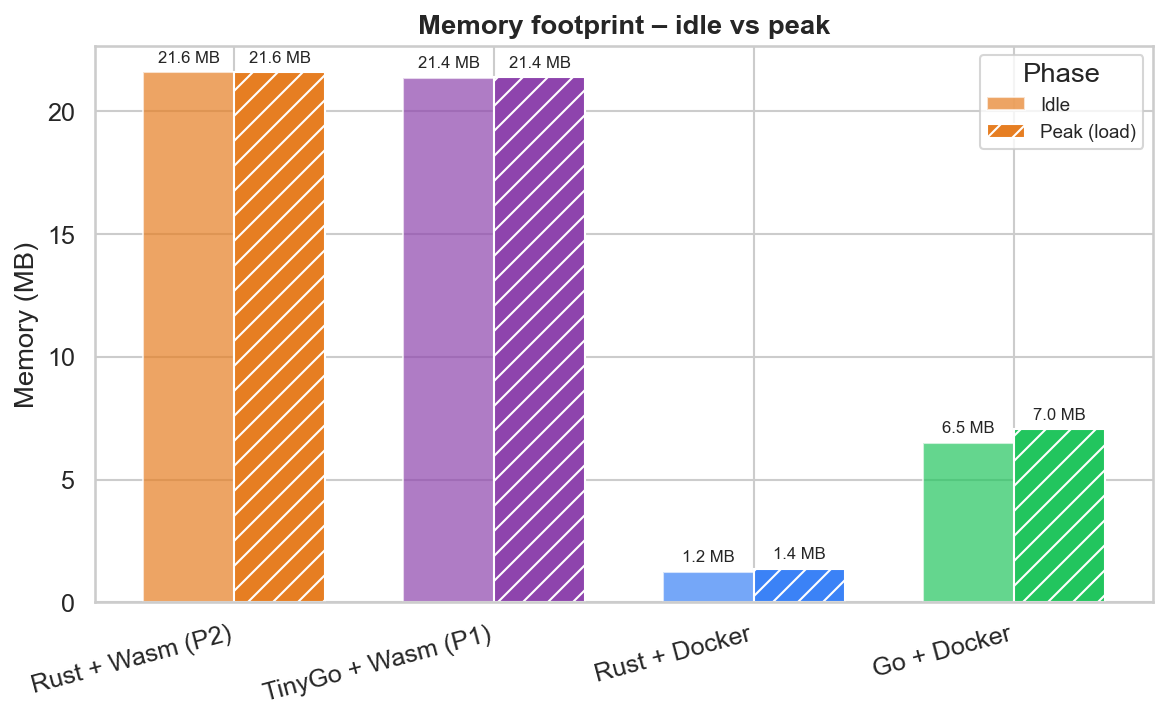
\includegraphics[width=0.49\textwidth]{figures/02-memory-bandwidth/limited/memory.png}%
        \label{fig:memory_mb_lim}}
    \caption{Container \acs{RSS} memory footprint per variant (idle vs.\ peak under load) in limited mode.}
    \label{fig:memory_limited}
\end{figure}

Figure~\ref{fig:memory_limited} reports per-variant \acs{RSS} at idle and at peak load for both benchmarks. The Wasm variants carry a substantially higher resident-memory footprint than the Docker variants: on the prime sieve, wasm-rust holds ~23\,MB and wasm-tinygo ~22\,MB at idle and peak, against docker-rust's ~2--3\,MB and docker-golang's ~9\,MB---a Wasm linear-memory tax of roughly 20\,MB relative to docker-rust. The memory-bandwidth workload shows the same pattern (wasm-rust ~21\,MB, wasm-tinygo ~21\,MB, docker-rust ~1\,MB, docker-golang ~7\,MB). Three observations follow:

\begin{itemize}
    \item Spin's \acs{RSS} includes Wasmtime's \acs{JIT} compilation context and the \acs{Wasm} component's pre-allocated linear-memory region, both of which the Docker variants do not pay.
    \item Under \texttt{spec.replicas:~1} a single pod hosts a single Wasmtime instance; horizontal scaling provisions additional pods, so aggregate \acs{RSS} scales roughly linearly with the replica count while per-pod \acs{RSS} stays approximately constant.
    \item docker-rust consistently exhibits the lowest \acs{RSS} (~1--3\,MB) because it ships only the stripped Tokio executable on a \texttt{scratch} base, with no garbage collector and no language runtime metadata.
\end{itemize}

\begin{figure}[htbp]
    \centering
    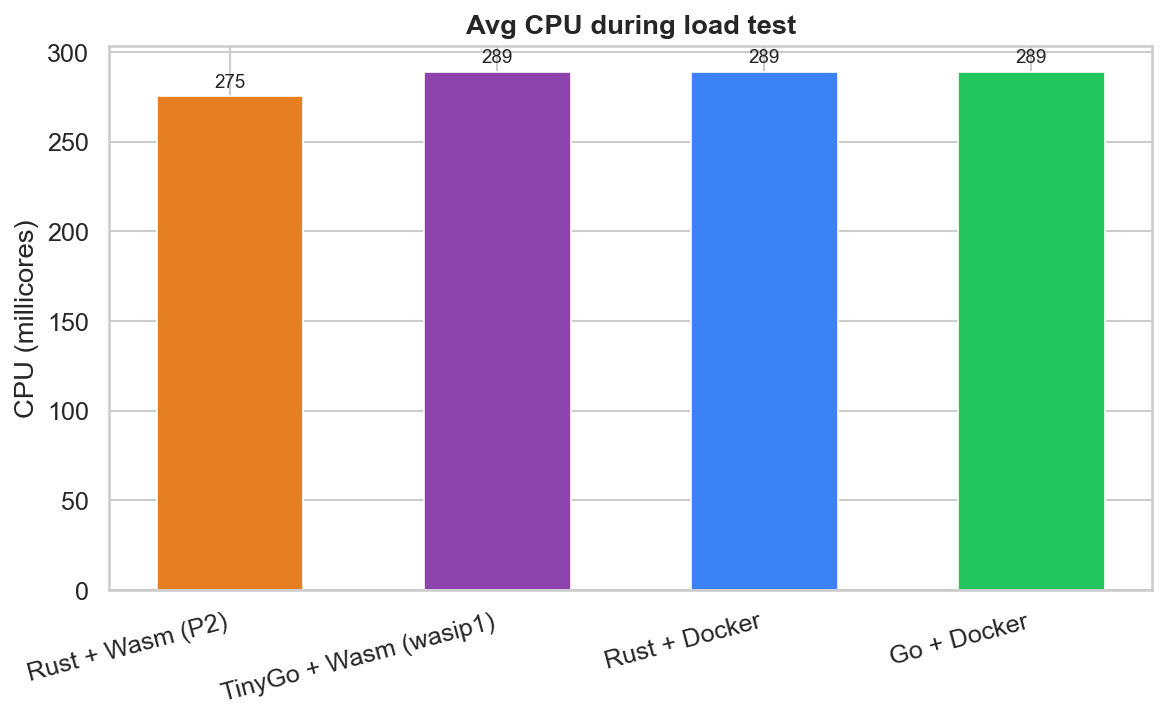
\includegraphics[width=0.75\textwidth]{figures/01-prime-sieve/limited/cpu.png}
    \caption{\acs{CPU} consumption (average millicores during the k6 hold phase) per variant for the prime-sieve workload. The memory-bandwidth experiment does not emit a dedicated \acs{CPU} chart because its runtime cost is dominated by the SHA-256 hash stage and is reported indirectly through the latency curves in Figure~\ref{fig:latency_limited}.}
    \label{fig:cpu_ps_lim}
\end{figure}

Figure~\ref{fig:cpu_ps_lim} highlights a complementary trade-off for the prime-sieve workload: docker-rust averages ~1230\,mcores during the load window---the highest of any variant---because Tokio spawns multiple OS threads to service the request stream, whereas wasm-rust achieves comparable throughput at ~429\,mcores under the same hold-phase load. wasm-tinygo sits essentially next to wasm-rust at ~425\,mcores, and docker-golang at ~948\,mcores. The Wasm variants therefore consume roughly one-third of docker-rust's CPU cycles per request at similar throughput.

\subsection{Observed Memory Profile}

The two figures expose a clean trade-off rather than a strict winner: the Wasm variants pay a per-pod linear-memory footprint premium of roughly 20\,MB (rooted in Wasmtime's \acs{JIT} context and the Wasm component's pre-allocated linear-memory region), while the docker-rust variant inverts the trade-off by holding the lowest \acs{RSS} but consuming the most CPU cycles per request. This matters for capacity planning: on a memory-constrained host, the Docker variants pack more replicas per node; on a \acs{CPU}-constrained host, the Wasm variants leave more headroom per replica.

\section{HTTP Fan-out Results (I/O-Bound)}
\label{sec:eval_fanout}

The HTTP fan-out workload (Section~\ref{sec:http_fanout_workload}) extends the evaluation to the I/O-bound regime, the third workload class promised in the task description. Each inbound request is amplified into $N$ concurrent outbound \acs{HTTP} GETs against the in-cluster \texttt{io-echo} backend, so per-request latency is dominated by outbound wait rather than \acs{CPU} work.

\begin{figure}[htbp]
    \centering
    \subfloat[\acs{OCI} image size.]{%
        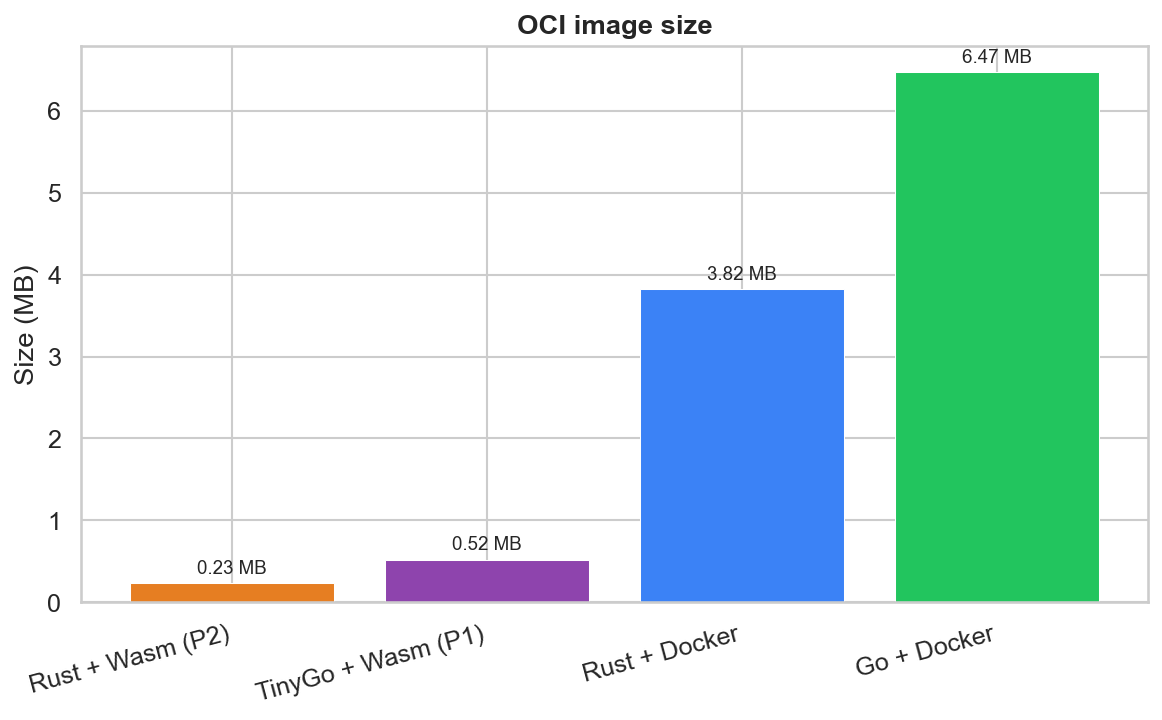
\includegraphics[width=0.49\textwidth]{figures/03-http-fanout/limited/image_size.png}%
        \label{fig:fanout_image_size}}
    \hfill
    \subfloat[Binary artefact size.]{%
        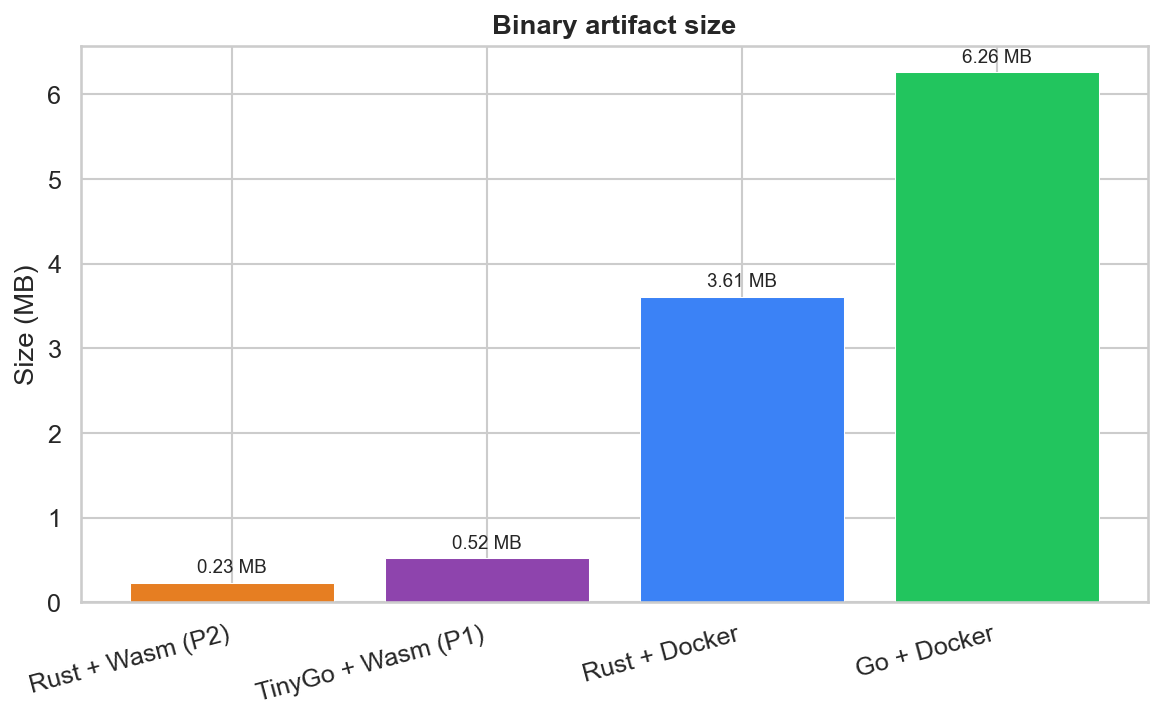
\includegraphics[width=0.49\textwidth]{figures/03-http-fanout/limited/binary_size.png}%
        \label{fig:fanout_binary_size}}
    \caption{HTTP fan-out: image and binary artefact sizes.}
    \label{fig:fanout_sizes}
\end{figure}

\begin{figure}[htbp]
    \centering
    \subfloat[Cold start.]{%
        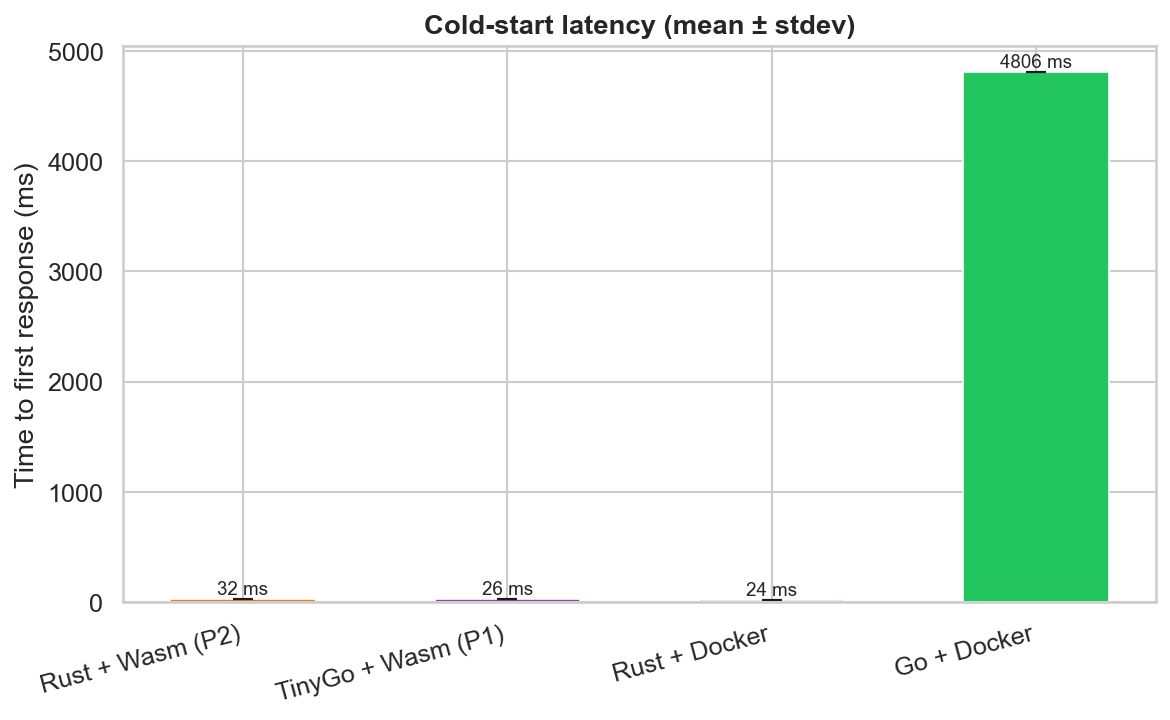
\includegraphics[width=0.49\textwidth]{figures/03-http-fanout/limited/cold_start.png}%
        \label{fig:fanout_cold}}
    \hfill
    \subfloat[Warm start.]{%
        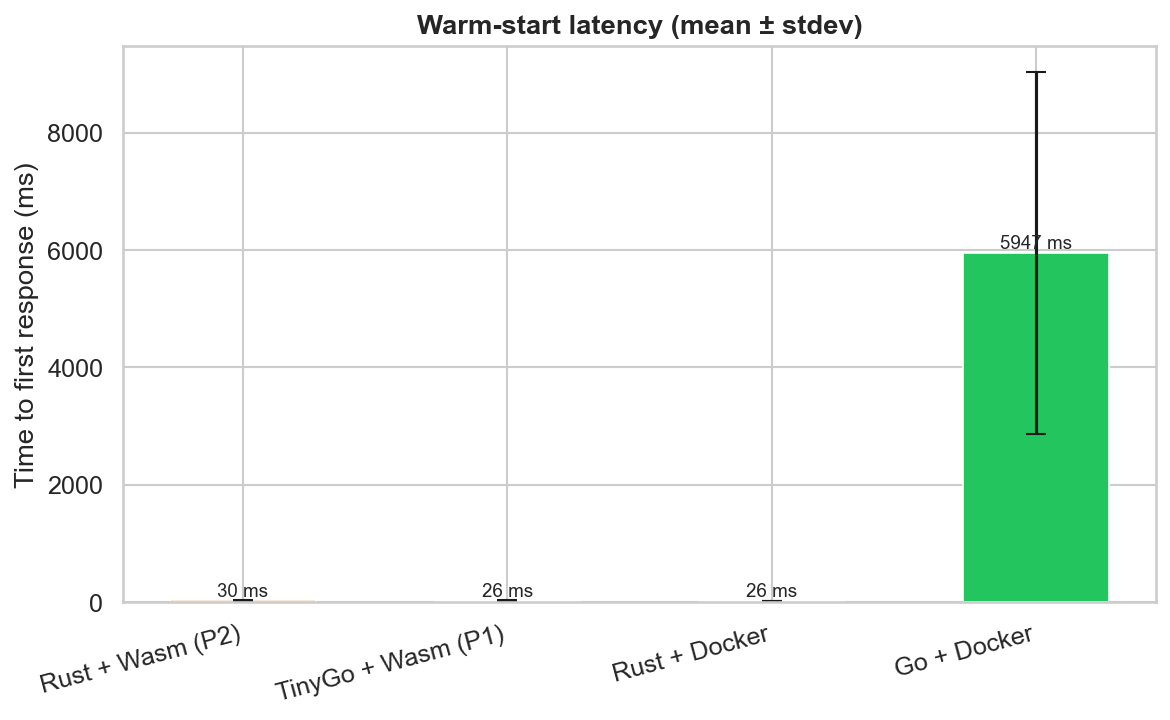
\includegraphics[width=0.49\textwidth]{figures/03-http-fanout/limited/warm_start.png}%
        \label{fig:fanout_warm}}
    \caption{HTTP fan-out: cold-start and warm-start latency.}
    \label{fig:fanout_startup}
\end{figure}

\begin{figure}[htbp]
    \centering
    \subfloat[Throughput (limited).]{%
        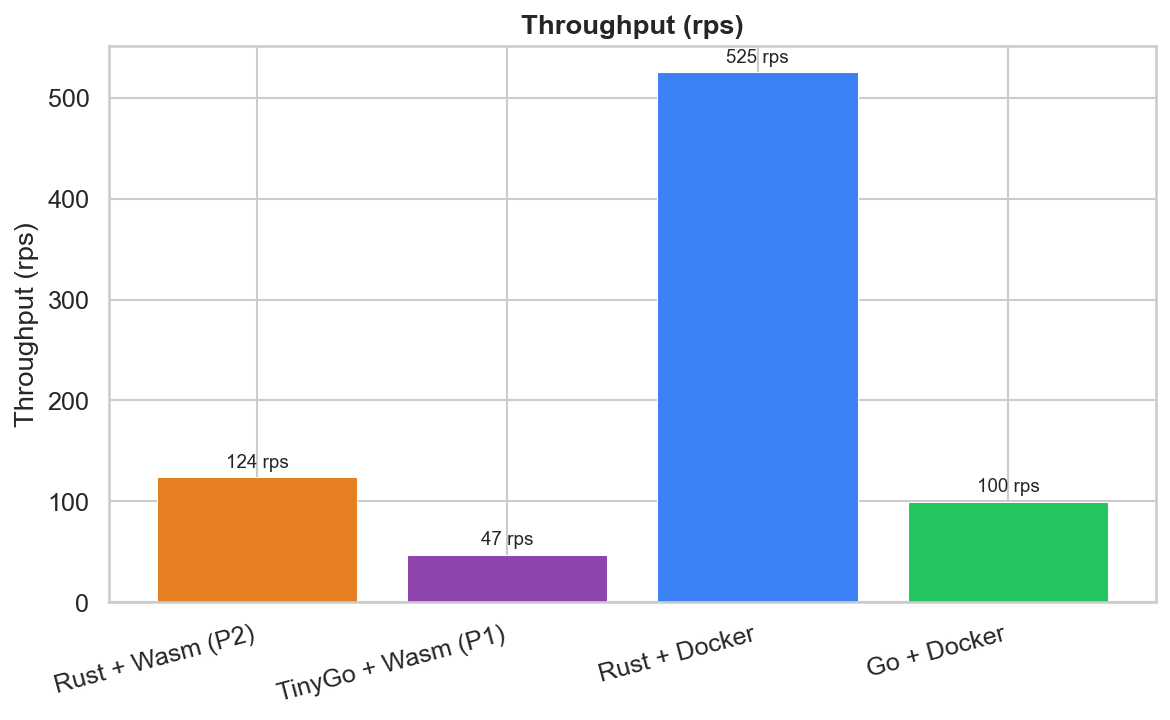
\includegraphics[width=0.49\textwidth]{figures/03-http-fanout/limited/throughput.png}%
        \label{fig:fanout_tput_lim}}
    \hfill
    \subfloat[Throughput (unlimited).]{%
        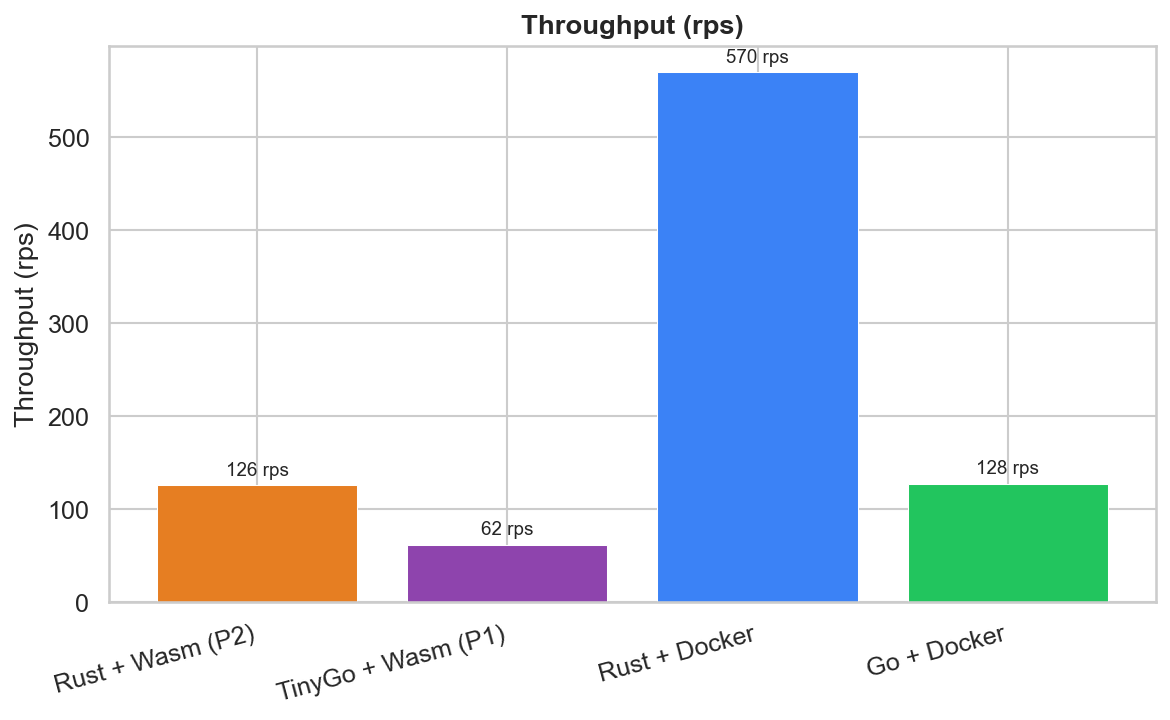
\includegraphics[width=0.49\textwidth]{figures/03-http-fanout/unlimited/throughput.png}%
        \label{fig:fanout_tput_unl}}
    \caption{HTTP fan-out: sustained throughput in both scaling modes.}
    \label{fig:fanout_throughput}
\end{figure}

\begin{figure}[htbp]
    \centering
    \subfloat[Latency (limited).]{%
        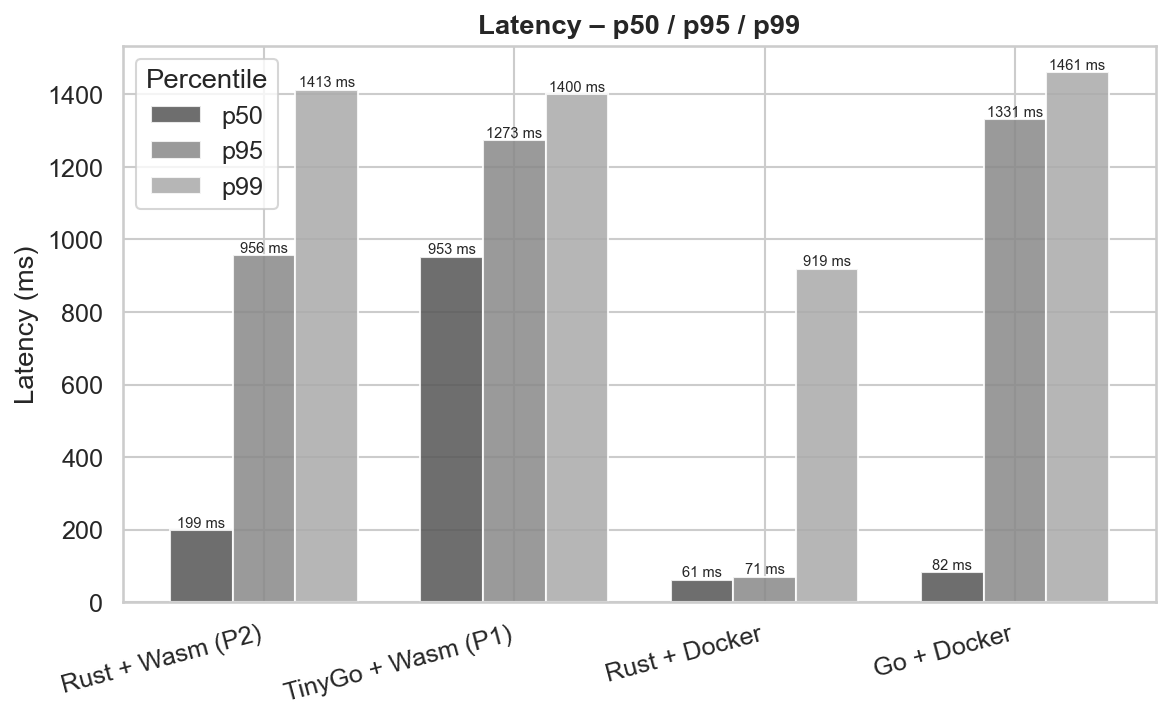
\includegraphics[width=0.49\textwidth]{figures/03-http-fanout/limited/latency.png}%
        \label{fig:fanout_lat_lim}}
    \hfill
    \subfloat[Latency (unlimited).]{%
        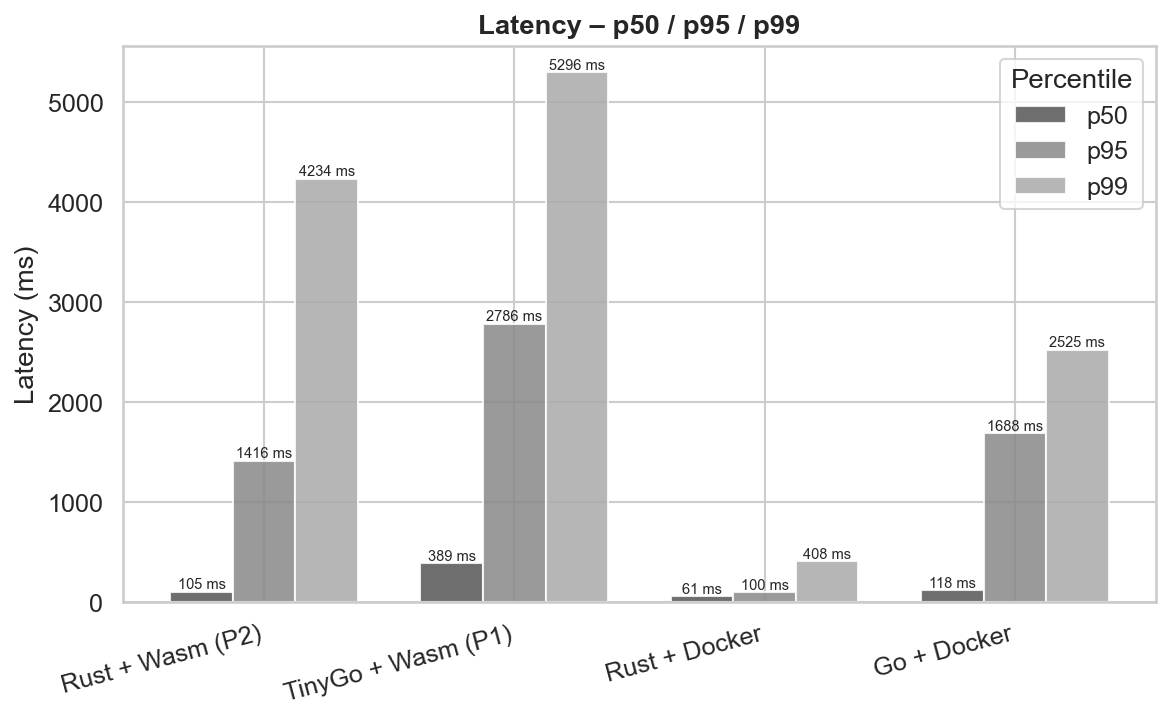
\includegraphics[width=0.49\textwidth]{figures/03-http-fanout/unlimited/latency.png}%
        \label{fig:fanout_lat_unl}}
    \caption{HTTP fan-out: p50/p95/p99 end-to-end latency.}
    \label{fig:fanout_latency}
\end{figure}

\begin{figure}[htbp]
    \centering
    \subfloat[Error rate.]{%
        \includegraphics[width=0.49\textwidth]{figures/03-http-fanout/limited/error_rate.png}%
        \label{fig:fanout_err}}
    \hfill
    \subfloat[Memory footprint (idle vs peak).]{%
        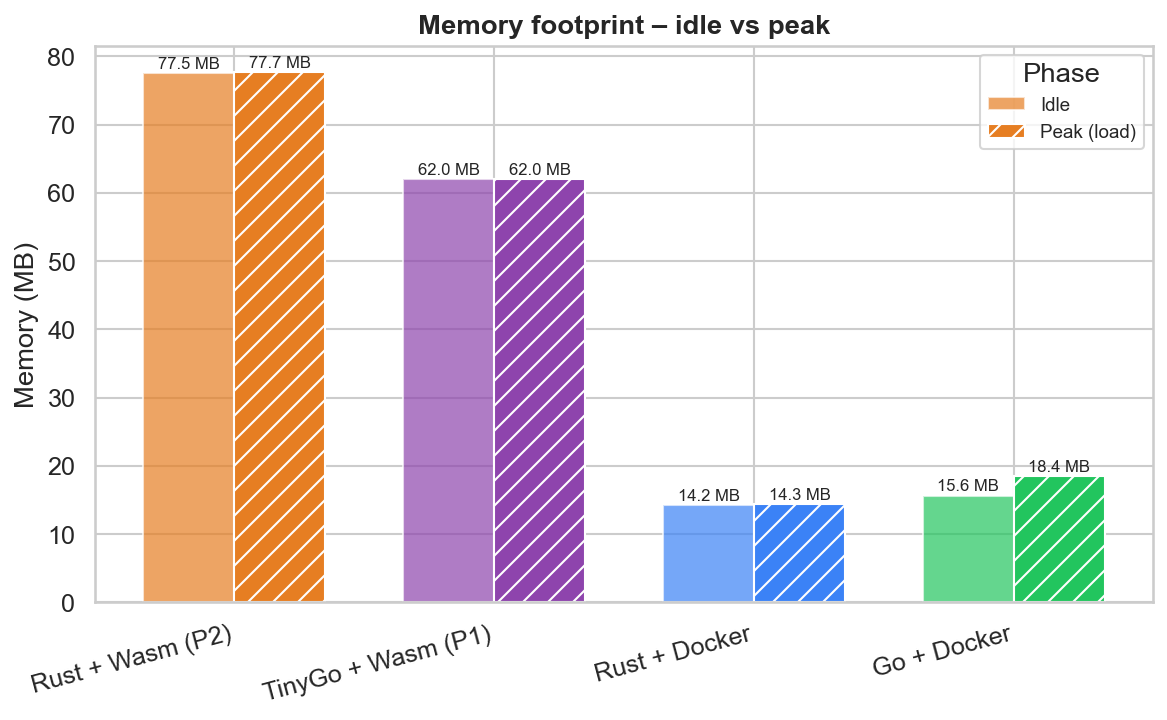
\includegraphics[width=0.49\textwidth]{figures/03-http-fanout/limited/memory.png}%
        \label{fig:fanout_mem}}
    \caption{HTTP fan-out: error rate and memory footprint.}
    \label{fig:fanout_quality}
\end{figure}

Under the default load profile (50~\acp{VU}, $N=5$, $\Delta=50$\,ms backend delay), the four variants distribute as follows: docker-rust sustains 525\,rps on the concurrent \texttt{reqwest~+~join\_all} path; wasm-rust achieves 124\,rps via \texttt{spin\_sdk::http::send~+~futures::join\_all}; docker-golang reaches 100\,rps with \texttt{net/http~+~goroutines~+~WaitGroup}; and wasm-tinygo lags at 47\,rps because TinyGo's wasip1 runtime forces sequential dispatch (Section~\ref{sec:impl_http_fanout}). The variant ordering in the I/O-bound regime is therefore not the same as in the \acs{CPU}-bound regime: docker-rust now leads by a wide margin (~4$\times$ over wasm-rust), wasm-rust beats docker-golang despite the older WASI~P1 runtime story predicting the reverse, and wasm-tinygo lags both by an additional factor of ~2.5 because TinyGo's wasip1 runtime forces serial outbound dispatch. The bottleneck is concurrent outbound dispatch efficiency, not single-handler throughput. This finding is revisited in Section~\ref{sec:discussion_fanout}.

\section{JSON Round-trip Results}
\label{sec:eval_jsontx}

The \acs{JSON} round-trip workload (Section~\ref{sec:json_roundtrip_workload}) stresses serialization and small-object allocation under varying request-body size. The result panels follow the standard layout, plus the dedicated \texttt{n\_sweep.png} chart (Figure~\ref{fig:jsontx_nsweep}) showing throughput-vs-$N$ on a logarithmic horizontal axis.

\begin{figure}[htbp]
    \centering
    \subfloat[\acs{OCI} image size.]{%
        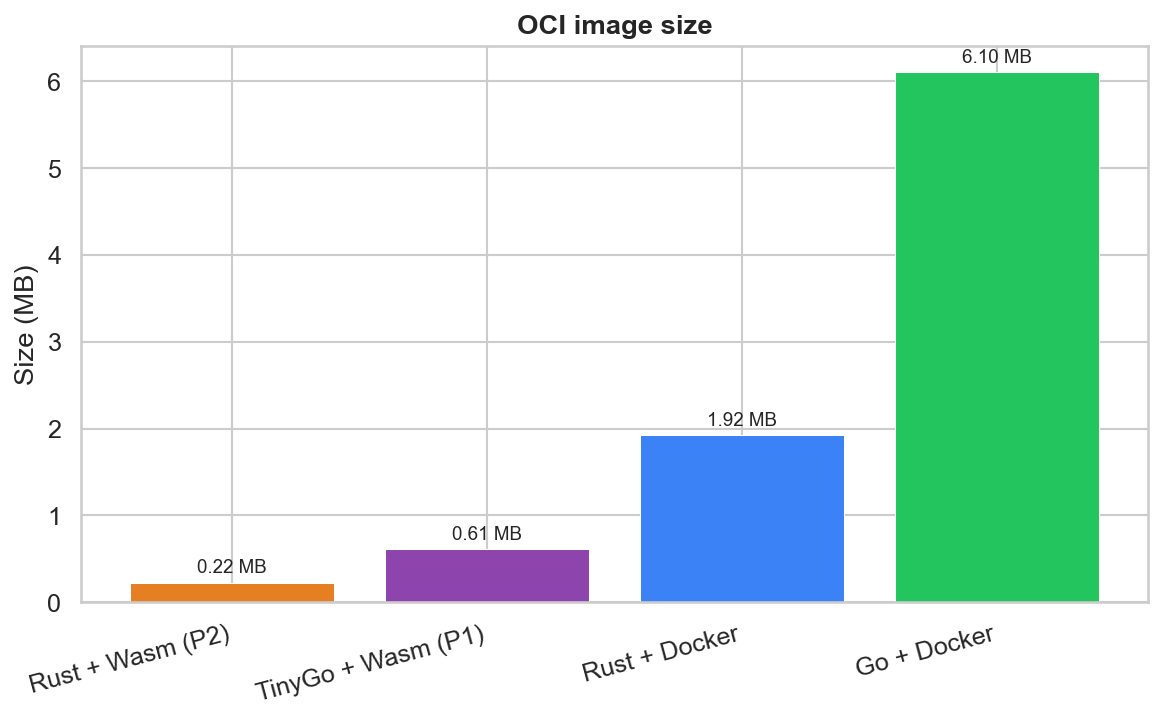
\includegraphics[width=0.49\textwidth]{figures/04-json-roundtrip/limited/image_size.png}%
        \label{fig:jsontx_image_size}}
    \hfill
    \subfloat[Binary artefact size.]{%
        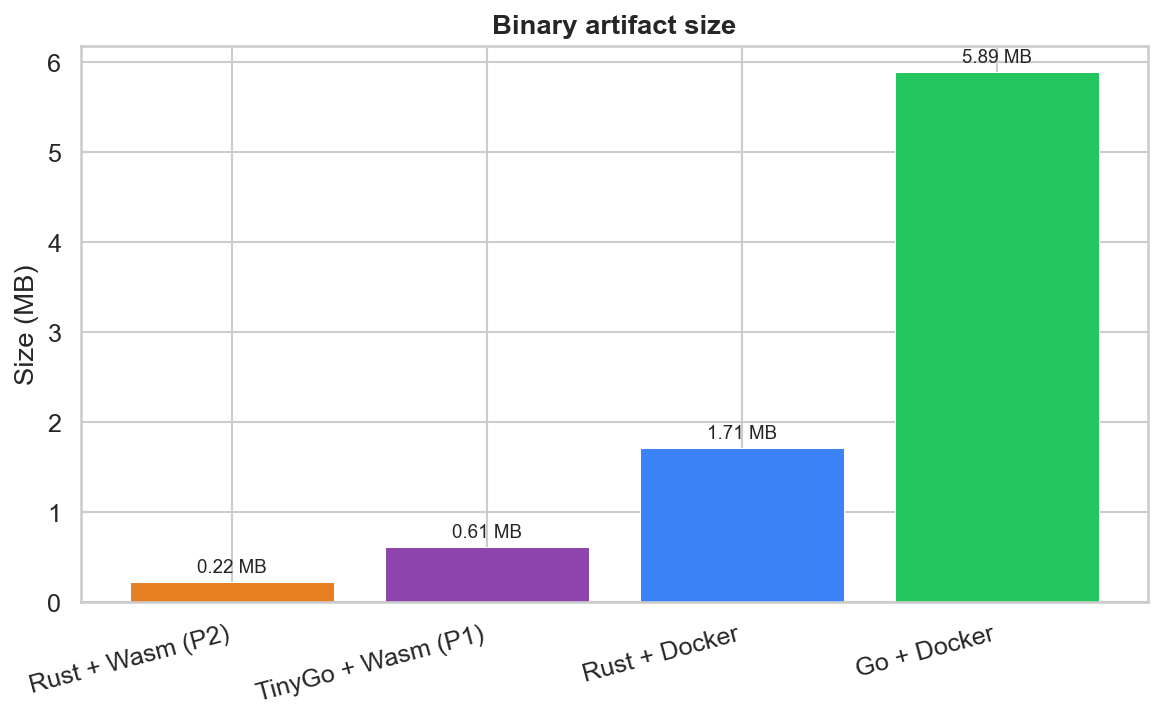
\includegraphics[width=0.49\textwidth]{figures/04-json-roundtrip/limited/binary_size.png}%
        \label{fig:jsontx_binary_size}}
    \caption{JSON round-trip: image and binary artefact sizes.}
    \label{fig:jsontx_sizes}
\end{figure}

\begin{figure}[htbp]
    \centering
    \subfloat[Cold start.]{%
        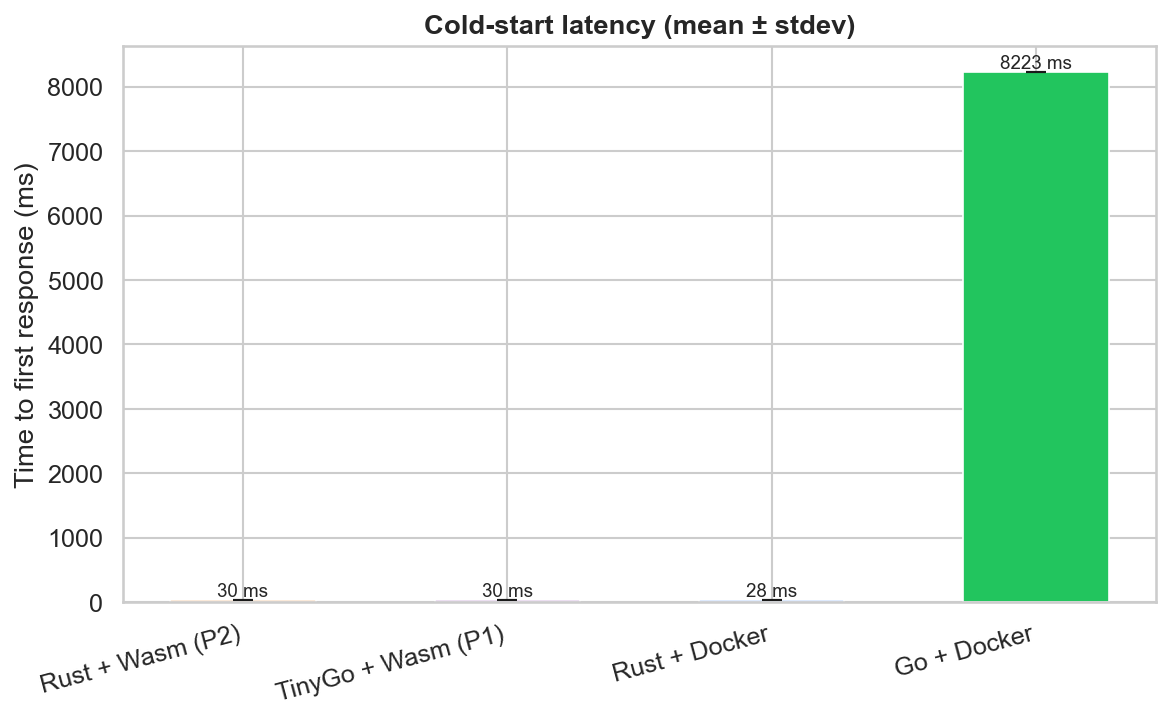
\includegraphics[width=0.49\textwidth]{figures/04-json-roundtrip/limited/cold_start.png}%
        \label{fig:jsontx_cold}}
    \hfill
    \subfloat[Warm start.]{%
        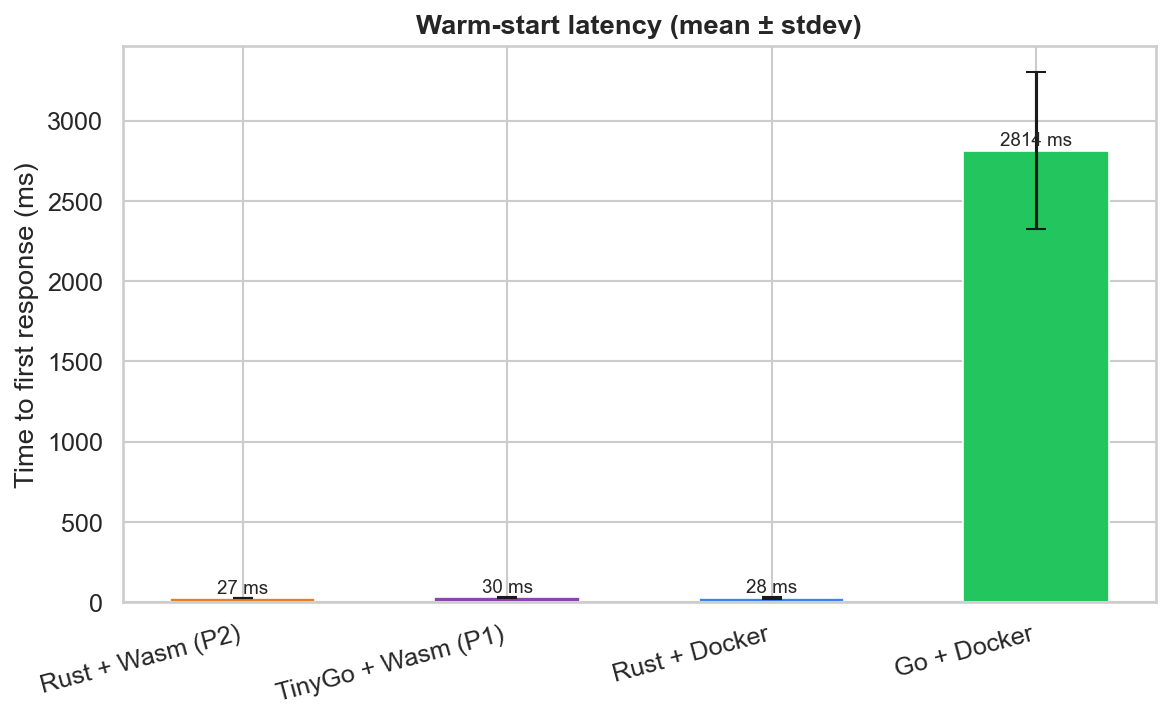
\includegraphics[width=0.49\textwidth]{figures/04-json-roundtrip/limited/warm_start.png}%
        \label{fig:jsontx_warm}}
    \caption{JSON round-trip: cold-start and warm-start latency.}
    \label{fig:jsontx_startup}
\end{figure}

\begin{figure}[htbp]
    \centering
    \subfloat[Throughput (limited).]{%
        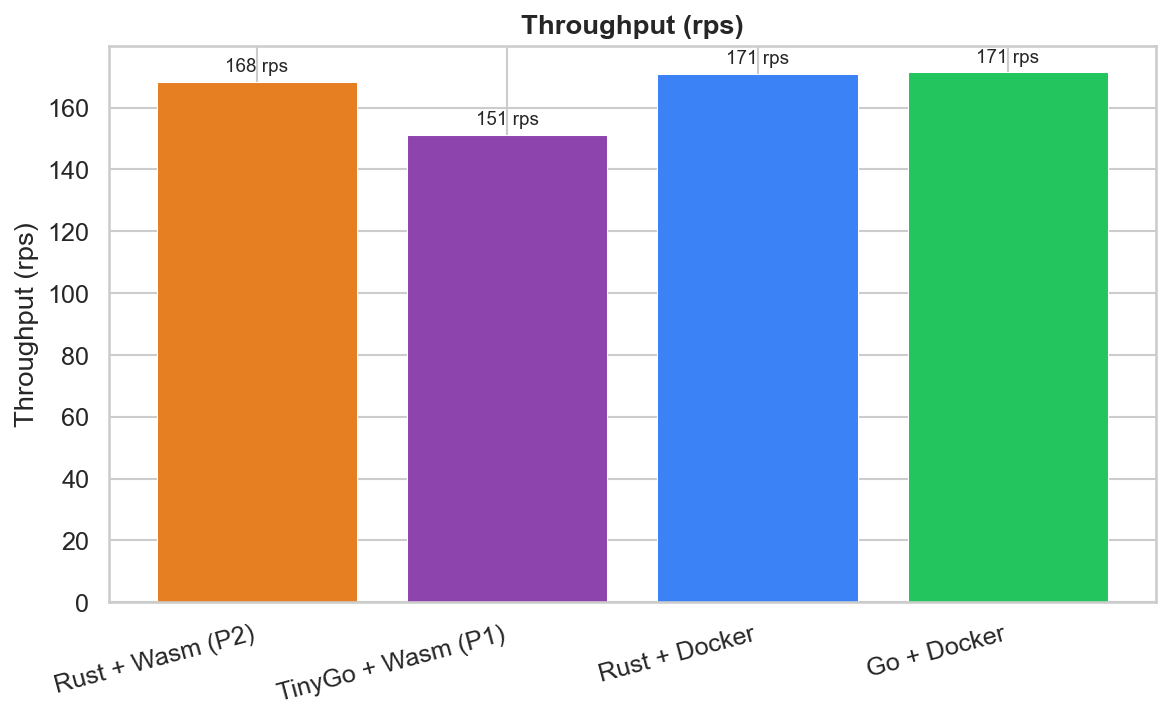
\includegraphics[width=0.49\textwidth]{figures/04-json-roundtrip/limited/throughput.png}%
        \label{fig:jsontx_tput_lim}}
    \hfill
    \subfloat[Throughput (unlimited).]{%
        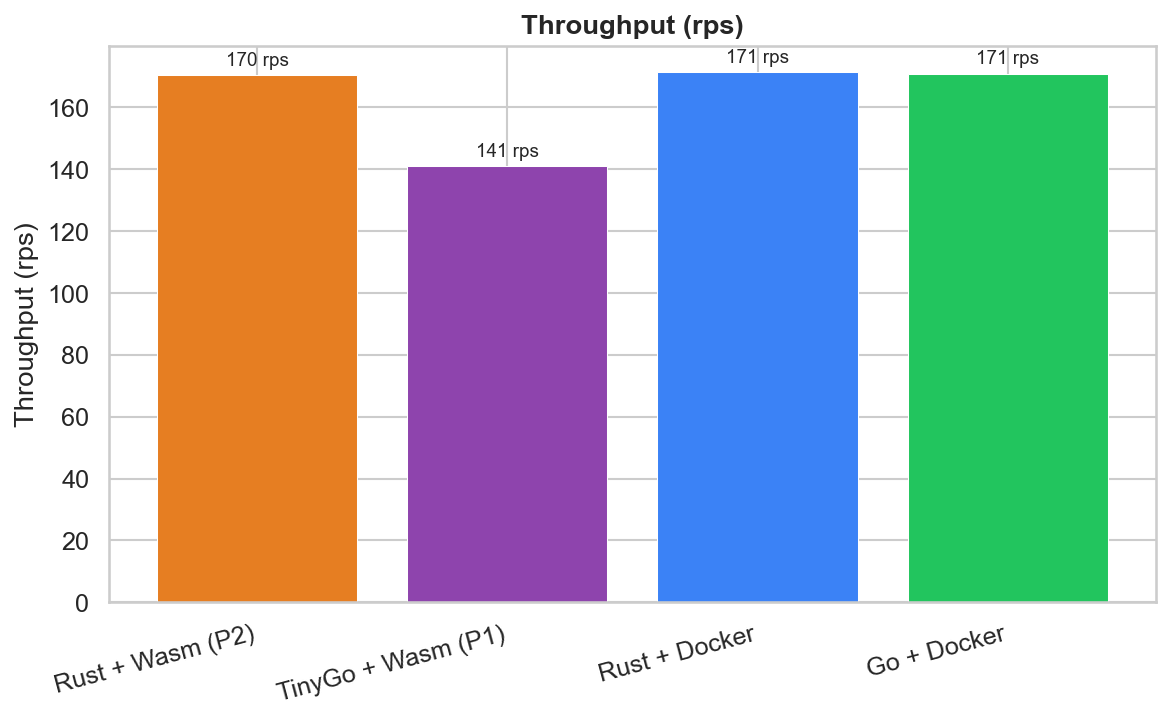
\includegraphics[width=0.49\textwidth]{figures/04-json-roundtrip/unlimited/throughput.png}%
        \label{fig:jsontx_tput_unl}}
    \caption{JSON round-trip: sustained throughput in both scaling modes.}
    \label{fig:jsontx_throughput}
\end{figure}

\begin{figure}[htbp]
    \centering
    \subfloat[Latency (limited).]{%
        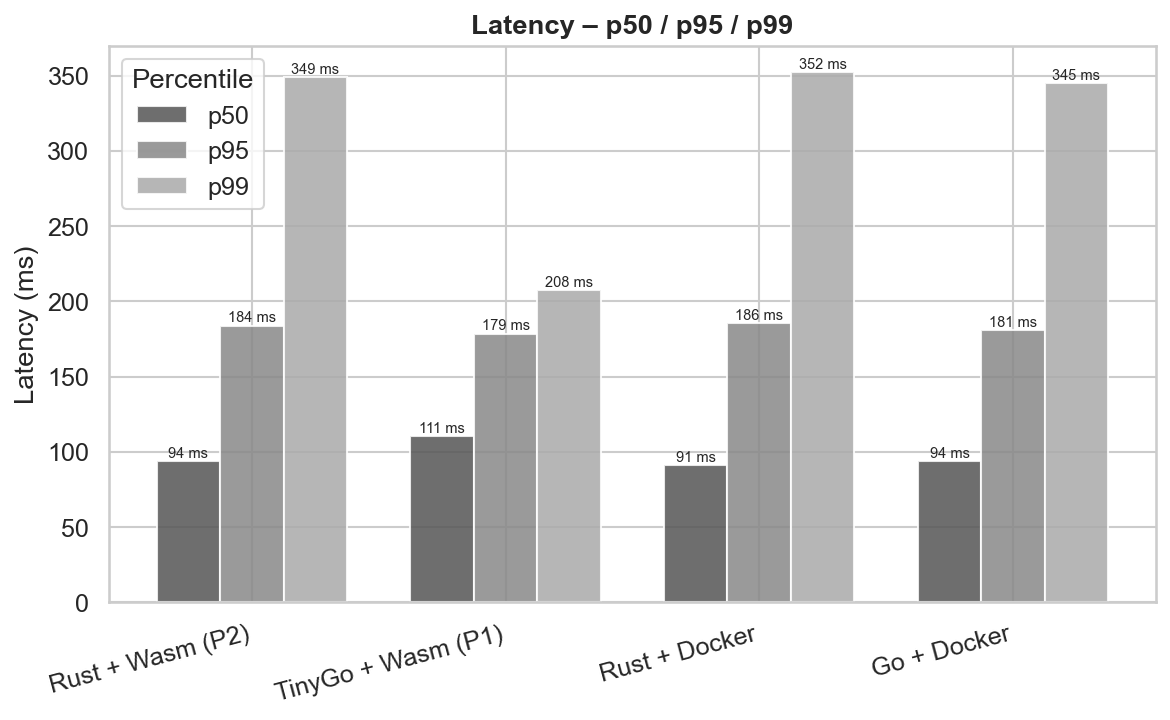
\includegraphics[width=0.49\textwidth]{figures/04-json-roundtrip/limited/latency.png}%
        \label{fig:jsontx_lat_lim}}
    \hfill
    \subfloat[Latency (unlimited).]{%
        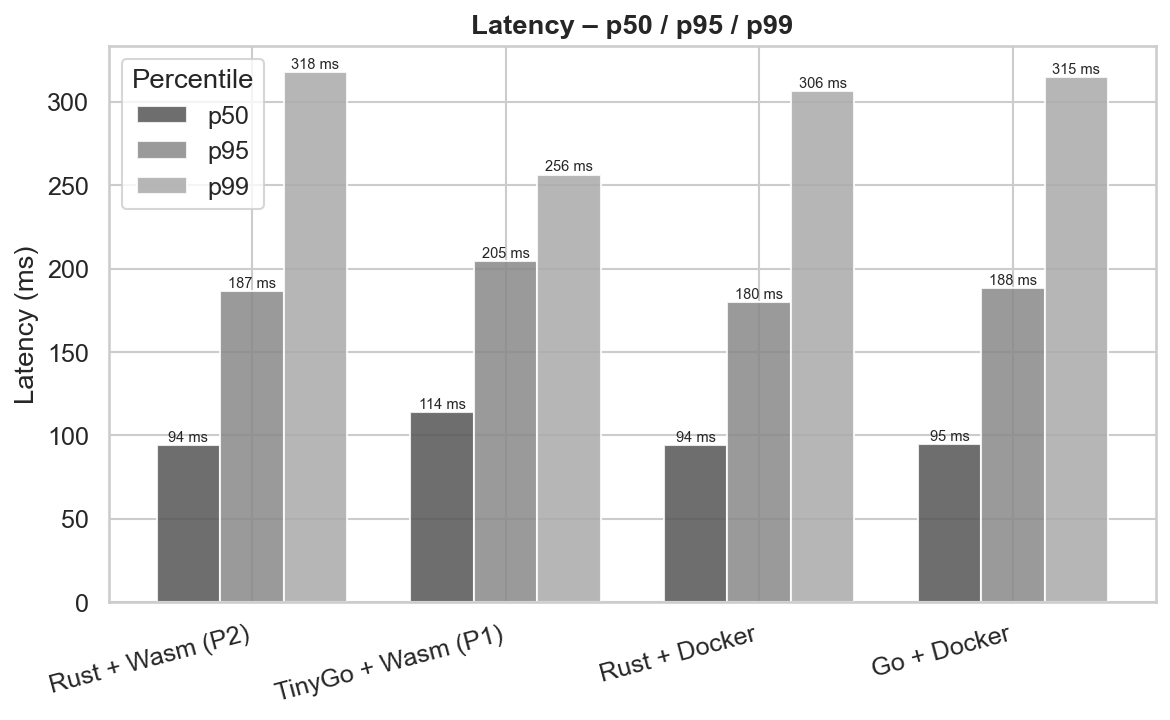
\includegraphics[width=0.49\textwidth]{figures/04-json-roundtrip/unlimited/latency.png}%
        \label{fig:jsontx_lat_unl}}
    \caption{JSON round-trip: p50/p95/p99 end-to-end latency.}
    \label{fig:jsontx_latency}
\end{figure}

\begin{figure}[htbp]
    \centering
    \subfloat[Error rate.]{%
        \includegraphics[width=0.49\textwidth]{figures/04-json-roundtrip/limited/error_rate.png}%
        \label{fig:jsontx_err}}
    \hfill
    \subfloat[Memory footprint (idle vs peak).]{%
        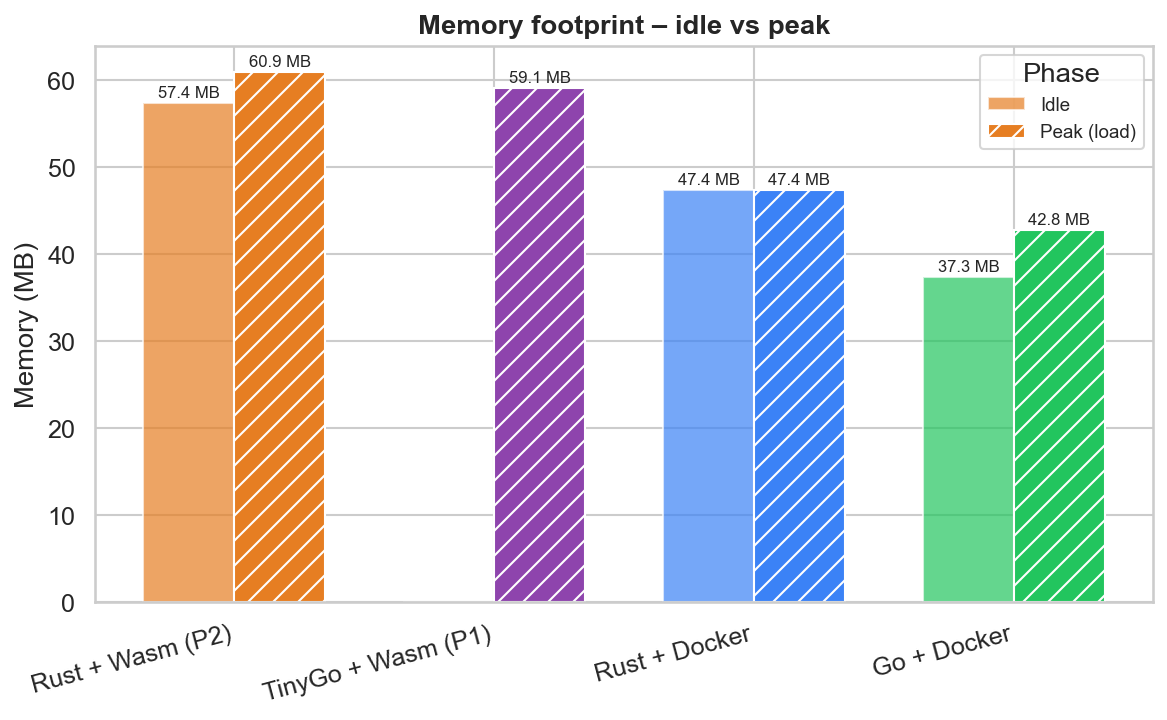
\includegraphics[width=0.49\textwidth]{figures/04-json-roundtrip/limited/memory.png}%
        \label{fig:jsontx_mem}}
    \caption{JSON round-trip: error rate and memory footprint.}
    \label{fig:jsontx_quality}
\end{figure}

\begin{figure}[htbp]
    \centering
    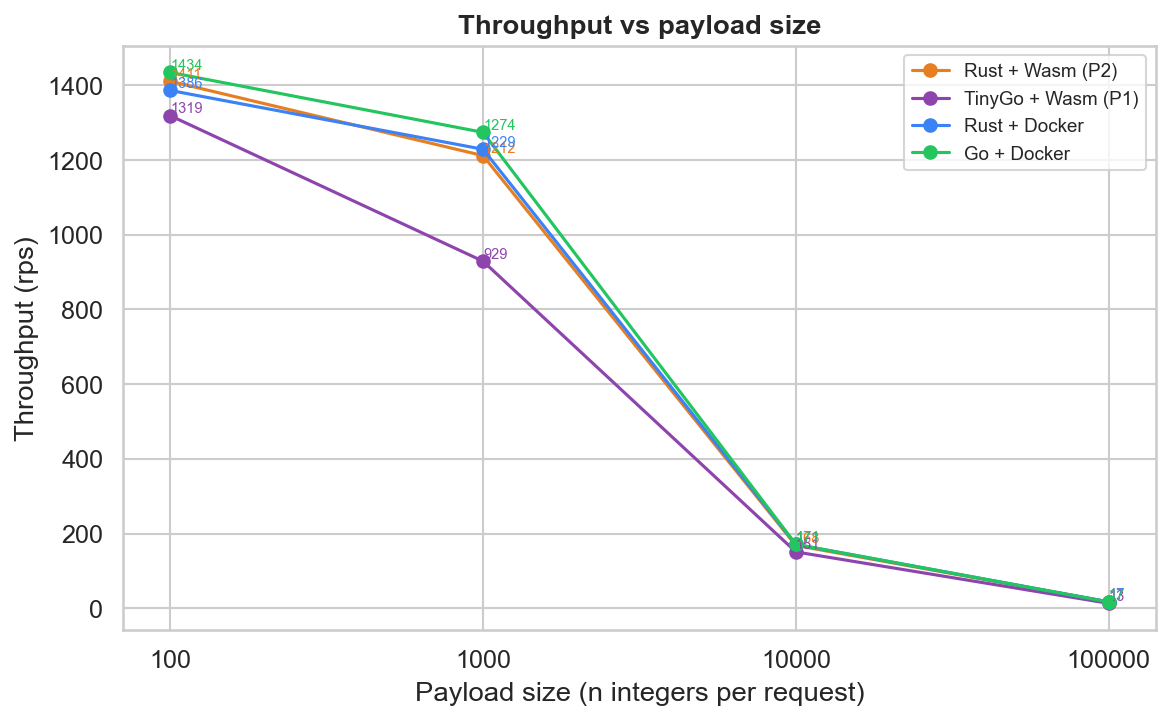
\includegraphics[width=0.75\textwidth]{figures/04-json-roundtrip/limited/n_sweep.png}
    \caption{JSON round-trip: throughput vs.\ request-array length $N$ (log-scale horizontal axis), one curve per variant. The sweep exposes the per-byte cost of the host-to-guest \acs{HTTP}-body copy across the \acs{WASI}~P2 boundary as well as the allocator's behaviour under churn from many small \acs{JSON} objects.}
    \label{fig:jsontx_nsweep}
\end{figure}

At small $N$ ($N=100$) all four variants serve nearly the same throughput (~1300--1430\,RPS) because the parse/sort/aggregate cost is dwarfed by the \acs{HTTP} framing overhead. As $N$ grows, the wasm-rust, docker-rust, and docker-golang curves stay nearly indistinguishable from each other: at $N=10\,000$ they sit within 3\,RPS of one another (~168--171\,RPS), and at $N=100\,000$ all three are at ~17\,RPS. The wasm-tinygo curve separates from the other three at every $N$ above 100, lagging by ~25\% at $N=1000$ and by ~12\% at $N=10\,000$; at $N=100\,000$ the spread between the fastest (docker-rust at 17.4\,RPS) and slowest (wasm-tinygo at 13.5\,RPS) variant is 1.29$\times$. The flatness of the wasm-rust curve relative to docker-rust is the headline result: under \acs{WASI}~P2 with \texttt{serde\_json}, the per-byte host-to-guest \acs{HTTP}-body copy is not measurable as a slope divergence at payloads up to 100\,000 i64s---it would only become legible at request bodies in the 10--100\,MiB range, which exceeds the scope of this study. The visible separation between wasm-tinygo and the other three is attributable to TinyGo's conservative \acs{GC} per-object allocator overhead, not to the \acs{WASI}~P2 boundary itself.

\section{Developer Experience}
\label{sec:eval_dx}

This section provides the qualitative assessment of the engineering effort required to build, test, and deploy each variant (addressing \acs{RQ4}). Four dimensions are evaluated on a four-point friction scale (Low / Medium / High / Very High). Table~\ref{tab:dx_assessment} summarises the assessment.

\begin{table}[htbp]
    \centering
    \caption{Developer experience friction assessment per variant and dimension.}
    \label{tab:dx_assessment}
    \adjustbox{max width=\linewidth}{%
    \begin{tabular}{lllll}
        \hline
        \textbf{Dimension}            & \textbf{wasm-rust} & \textbf{wasm-tinygo} & \textbf{docker-rust} & \textbf{docker-golang} \\
        \hline
        Toolchain setup               & Low-Medium & Medium     & Low-Medium & Low    \\
        Dependency compatibility      & Low        & Low        & Low        & Low    \\
        K8s cluster integration       & Low-Medium & Low-Medium & Low        & Low    \\
        Debugging and observability   & Medium     & Medium     & Low        & Low    \\
        \hline
    \end{tabular}}
\end{table}

\subsection{Toolchain Setup}

The Docker variants require only a standard \texttt{docker build} workflow. Go~1.26's toolchain is a single binary download; Rust~1.94 requires \texttt{rustup} but is well-documented and cross-platform.

The wasm-rust variant adds \texttt{cargo-component} (\texttt{cargo install cargo-component}) and the \texttt{wasm32-wasip2} Rust target (\texttt{rustup target add wasm32-wasip2}). The \texttt{spin} \acs{CLI} is required for \texttt{spin registry push}. These are all first-party tools with stable documentation. The friction is rated Low-Medium because \texttt{cargo-component} is a separate install step not yet integrated into the \texttt{cargo} core toolchain.

The wasm-tinygo variant requires TinyGo~0.40.0 (installed as a \texttt{.tar.gz} release, no stable \texttt{apt} package on Ubuntu) and the \texttt{spin} \acs{CLI}. The \texttt{-target=wasip1} flag is required: TinyGo's \texttt{wasip2} target hardwires the \texttt{wasi:cli/command} world and cannot export \texttt{wasi:http/incoming-handler}. The Spin Go \acs{SDK} (\texttt{github.com/spinframework/spin-go-sdk/v2}) provides \texttt{spinhttp.Handle()} via a \acs{CGo} layer, exporting \texttt{fermyon:spin/inbound-http}, allowing the TinyGo handler to use standard \texttt{net/http} types.

\subsection{Dependency Compatibility}

The Docker variants had no dependency issues. All crates and packages compile without modification.

The wasm-rust variant uses only the \texttt{spin-sdk~=~"5.2.0"} crate and standard library dependencies. No proprietary socket crates are required; \texttt{wasm32-wasip2} is a Tier~2 stable Rust target since Rust~1.82.

The wasm-tinygo variant uses \texttt{spinhttp.Handle()} from the official Spin \acs{SDK} for Go (\texttt{github.com/spinframework/spin-go-sdk/v2}). Standard \texttt{net/http} types work without modification; no \texttt{//go:wasmimport} socket directives or custom \texttt{server.go} are required.

\subsection{Kubernetes Integration}

Docker variants require standard \acs{K8s} manifests with no special configuration.

The Spin variants require: (1) a cluster-level \texttt{RuntimeClass} object (\texttt{wasmtime-spin}), (2) the SpinOperator \acs{CRD} and Helm chart (installed once via \texttt{make deploy}), and (3) \texttt{SpinApp} \acs{CRD} manifests instead of standard \texttt{Deployment} + \texttt{Service} manifests. The \texttt{SpinApp} resource is more opinionated than a raw \texttt{Deployment} but conceptually simpler (no pod template, no replica management outside the \acs{CRD}). The cluster setup (\texttt{containerd-shim-spin-v2} installation, containerd plugin registration) is automated by \texttt{cloud-init.sh} and requires no manual intervention after initial provisioning.

The SpinKube integration is comparable in operational complexity to standard \acs{K8s} Helm-chart workflows: \texttt{containerd-shim-spin-v2} is a static binary installed by \texttt{cloud-init}, and the SpinOperator is delivered as a Helm chart with a single \texttt{kubectl apply} for the supporting \texttt{RuntimeClass} and \acs{CRD}s.

\subsection{Debugging and Observability}

Docker containers support the full debugging toolkit: \texttt{kubectl exec} for interactive shell access, \texttt{docker logs} for stdout/stderr, and native debuggers (Delve for Go, \texttt{rust-gdb} for Rust) can be attached to running processes.

Spin \acs{Wasm} pods support stdout/stderr log output (via \texttt{kubectl logs}). \texttt{kubectl exec} cannot open a shell into a \acs{Wasm} pod because the \acs{WASI} environment does not expose a shell binary or an interactive \acs{PTY} interface. No debugger can attach to a running Wasmtime process from outside the \acs{Wasm} sandbox. The absence of debugger support increases the iteration cycle when diagnosing runtime failures; in practice most issues surface at build time as standard Rust or Go compilation errors rather than at runtime.

\section{Summary of Findings}
\label{sec:eval_summary}

\textit{Quantitative summary will be populated once benchmark measurements are complete. The qualitative developer experience findings are complete above.}

The key qualitative finding is that SpinKube/\acs{WASI}~P2 provides a low-friction Wasm development experience. All four dependency compatibility ratings sit at Low because standard \texttt{net/http} and standard Rust networking abstractions work correctly without proprietary workarounds. K8s integration friction is low because \texttt{containerd-shim-spin-v2} is a static binary installed by \texttt{cloud-init} without source compilation. The remaining friction (Medium for toolchain setup and debugging) is inherent to the \acs{Wasm}/\acs{WASI} execution model and is expected to decrease as the ecosystem matures.

\chapter{Discussion and Future Work}
\label{chap:discussion}

\section{The Trade-off: Maturity vs. Efficiency}
Discussion on the "Ecosystem Gap." While Wasm is more efficient, Golang/Docker has vastly superior library support and tooling availability.

\section{Security Implications}
How the "deny-by-default" security posture of Wasm changes the cluster security model compared to root-access risks in Docker.

\section{Migration Recommendations}
Guidelines for companies (like Akamai or Cloudflare customers) on when to switch to Wasm (e.g., high-scale serverless functions) versus staying with Docker (stateful monoliths).
\chapter{Conclusion}
\label{chap:conclusion}
Summary of findings confirming whether Wasm/Rust serves as a viable alternative for the specific use case of high-density microservices.

% 4. Backmatter & Appendices
\appendix
\chapter{Reproducibility}
\label{app:reproducibility}

\section{Abstract}

The artefacts supporting this thesis are distributed across three public Git repositories: an infrastructure repository that provisions a single-node Kubernetes 1.34 cluster on Hetzner Cloud via Terraform plus \texttt{cloud-init} plus \texttt{kubeadm}; an experiments repository containing the four benchmark variants (\texttt{wasm-rust}, \texttt{wasm-tinygo}, \texttt{docker-rust}, \texttt{docker-golang}) across the two stateless \acs{HTTP} workloads (prime sieve, memory bandwidth), the k6 load-generator scripts, and the Prometheus / chart-regeneration helpers; and this thesis source. The end-to-end reproduction path is two \texttt{make} invocations against the infrastructure repository followed by a per-benchmark \texttt{run\_experiment.sh} script in the experiments repository, on a single Hetzner ccx23 \acs{VM} (4 vCPU, 16\,GB \acs{RAM}). The multi-node scaling experiments referenced as future work in Section~\ref{sec:future_work_multinode} are deferred and are not part of this artefact.

\section{Artifact check-list (meta-information)}

\begin{description}
    \item[Program:] Sieve of Eratosthenes \acs{HTTP} service (benchmark 01) and heap-allocation~+~SHA-256 \acs{HTTP} service (benchmark 02), each implemented as four variants (\texttt{wasm-rust}, \texttt{wasm-tinygo}, \texttt{docker-rust}, \texttt{docker-golang}).
    \item[Compilation:] Rust 1.94 with \texttt{cargo} and \texttt{cargo-component}, Go 1.26, TinyGo 0.40.0 (\texttt{-target=wasip1 -gc=conservative -opt=2}).
    \item[Run-time environment:] Ubuntu 24.04 LTS, Kubernetes 1.34 via \texttt{kubeadm}, containerd 2.0.2, \texttt{containerd-shim-spin-v2} v0.17.0, Flannel CNI, local-path-provisioner.
    \item[Hardware:] One Hetzner Cloud ccx23 \acs{VM} (4$\times$ AMD EPYC vCPU, 16\,GB \acs{RAM}, 160\,GB NVMe), location \texttt{nbg1}.
    \item[Metrics:] Requests per second; end-to-end latency p50/p95/p99; cold- and warm-start latency; container \acs{RSS} at idle and at peak load; \acs{CPU} consumption in millicores; on-disk \acs{OCI} artifact size.
    \item[Output:] Per-variant \texttt{*\_summary.json} files (aggregate k6 metrics), per-variant \texttt{*\_k6.json} files (raw k6 output), and per-mode aggregates \texttt{cold\_start.json}, \texttt{warm\_start.json}, \texttt{resource\_metrics.json}, \texttt{image\_sizes.json}, together with the PNG charts under \texttt{thesis-experiments/results/0\{1,2\}-*/\{limited,unlimited\}/} that Chapter~\ref{chap:evaluation} embeds.
    \item[Experiments:] \texttt{01-prime-sieve} and \texttt{02-memory-bandwidth}, each run in both \emph{limited} (single worker thread / single replica) and \emph{unlimited} (\texttt{GOMAXPROCS=4}, \texttt{TOKIO\_WORKER\_THREADS=4}, \texttt{SpinApp~spec.replicas:~4}) modes.
    \item[Approximate disk space:] A few \acs{GB} total, dominated by raw k6 \acs{JSON} output and the Prometheus \acs{PVC}.
    \item[Approximate wall-clock to reproduce:] ${\sim}30$\,min for cluster provisioning, plus ${\sim}20$\,min per benchmark mode, totalling ${\sim}2$\,h end-to-end.
    \item[Publicly available:] Yes; the three repositories are cited as \cite{musaev2026thesisinfra, musaev2026thesisexperiments, musaev2026thesissource}.
\end{description}

\section{Description}
\subsection{How to access}
\label{sec:repro_how_to_access}

The complete set of artefacts supporting the experiments in this thesis is distributed across three public Git repositories hosted on GitHub. Each repository is referenced from its corresponding chapter; this subsection groups them together as a single point of entry.

\begin{itemize}
    \item \textbf{Infrastructure setup} \textendash{} \cite{musaev2026thesisinfra}.
          Kubernetes (\texttt{kubeadm}) and SpinKube cluster provisioning, Hetzner Cloud Terraform modules, cloud-init bootstrap scripts, and the \texttt{containerd}~/ \texttt{containerd-shim-spin-v2} installation manifests used to build the four-variant experimental cluster described in \hyperref[chap:implementation]{Chapter~\ref{chap:implementation}}.

    \item \textbf{Benchmark implementations and result data} \textendash{} \cite{musaev2026thesisexperiments}.
          The four primary benchmark variants (\texttt{docker-golang}, \texttt{docker-rust}, \texttt{wasm-rust}, \texttt{wasm-tinygo}), the k6 load-generator configurations, the Prometheus scrape rules, and the raw \texttt{results/} directory referenced throughout \hyperref[chap:evaluation]{Chapter~\ref{chap:evaluation}}.

    \item \textbf{Thesis source} \textendash{} \cite{musaev2026thesissource}.
          The \LaTeX{} source of this document, including all chapter \texttt{.tex} files, the bibliography, TikZ figure sources, and the build instructions in the \texttt{Makefile}.
\end{itemize}

All three repositories are tagged at the commit corresponding to thesis submission so that a reader can clone the exact state of the artefacts that produced the reported results.

\subsection{Hardware dependencies}
\label{sec:repro_hardware}

The single-node measurement environment requires one Hetzner Cloud ccx23 \acs{VM} (4$\times$ AMD EPYC vCPU, 16\,GB \acs{RAM}, 160\,GB NVMe \acs{SSD}). The Hetzner default 8-core account quota is sufficient. The Terraform module accepts the location \texttt{nbg1} (Nuremberg) by default; any other Hetzner Cloud location should work without changes. An admin workstation with outbound \acs{SSH} (port 22) and \texttt{kubectl} (port 6443) connectivity to the \acs{VM}'s public \acs{IP} is required for provisioning and benchmark execution. The deferred multi-node mode (Section~\ref{sec:future_work_multinode}) would require additional Hetzner instances under the same account, but is not exercised by this artefact.

\subsection{Software dependencies}
\label{sec:repro_software}

On the admin workstation: Terraform $\geq 1.6$, \texttt{kubectl} matching cluster version 1.34, Helm~3, \texttt{make}, Docker~26 (to build and push the two Docker variants to a registry), Rust~1.94 with \texttt{rustup target add wasm32-wasip2} and \texttt{cargo install cargo-component --locked}, Go~1.26, TinyGo~0.40.0 (installed from the upstream \texttt{.tar.gz} release; no stable \texttt{apt} package on Ubuntu), the Spin \acs{CLI} v3+, k6 (installable via the Grafana \texttt{apt} repository), and Python~3 with \texttt{matplotlib} for chart regeneration.

On the provisioned cluster, the following components are installed automatically by \texttt{cloud-init} and by the \texttt{make deploy} target and therefore do not need to be installed manually: containerd~2.0.2, \texttt{runc}~1.2.4, CNI plugins~1.6.2, \texttt{containerd-shim-spin-v2}~v0.17.0, \texttt{cert-manager}~v1.16.3, SpinOperator~v0.6.1 (Helm chart \texttt{spinframework/spin-operator}), and \texttt{kube-prometheus-stack} (community Helm chart, with the values in \texttt{observability-values.yaml}).

\section{Installation}
\label{sec:repro_installation}

The following procedure provisions the single-node cluster end-to-end. All \texttt{make} targets referenced below are defined in \texttt{thesis-infra-setup/Makefile} and are idempotent: re-running \texttt{make deploy} against an established cluster is a no-op.

\begin{enumerate}
    \item Clone the three repositories side-by-side under a common parent directory (for example \texttt{\textasciitilde/coding/master-thesis/}). The Terraform Makefile and the per-benchmark \texttt{run\_experiment.sh} scripts assume this sibling layout.
    \item Populate \texttt{thesis-infra-setup/terraform.tfvars} with a Hetzner Cloud API token (\texttt{hcloud\_token}), an \acs{SSH} public key (\texttt{ssh\_public\_key}), and the admin workstation's egress \acs{IP}/CIDR (\texttt{admin\_ip\_cidr}). Leave \texttt{worker\_count = 0}, which is the single-node default.
    \item Provision the cluster: \texttt{make up}. This runs \texttt{terraform apply}, waits for \texttt{cloud-init} to complete, runs \texttt{kubeadm init} for Kubernetes 1.34, installs the Flannel CNI plug-in and the local-path-provisioner, registers \texttt{containerd-shim-spin-v2} with containerd, and removes the control-plane taint so that the single node can also schedule workload pods.
    \item Fetch the cluster's kubeconfig: \texttt{make configure}. This writes \texttt{hetzner-thesis.yaml} into the repository root and rewrites the API-server endpoint to the \acs{VM}'s public \acs{IP}.
    \item Label the node for SpinKube pod scheduling: \texttt{make label}.
    \item Install the cluster add-ons: \texttt{make deploy}. This installs \texttt{cert-manager}~v1.16.3, the SpinOperator Helm chart (v0.6.1) together with the \texttt{wasmtime-spin} \texttt{RuntimeClass}, and \texttt{kube-prometheus-stack} parameterised by \texttt{observability-values.yaml} (5\,s scrape interval, Grafana exposed as a \acs{NodePort}).
    \item Sanity-check the runtime path: \texttt{make test} applies \texttt{test-spin.yaml} (a Spin ``hello'' sample) and expects an \acs{HTTP}~200 response.
\end{enumerate}

Steps~1--7 typically complete in ${\sim}30$\,minutes of wall-clock time.

\section{Experiment workflow}
\label{sec:repro_workflow}

The two benchmarks share the same four-variant structure, the same NodePort assignment (30081 \texttt{wasm-rust}, 30082 \texttt{wasm-tinygo}, 30083 \texttt{docker-rust}, 30084 \texttt{docker-golang}), and the same orchestrator script layout. They are run sequentially because the two benchmarks share NodePorts; the \texttt{02-memory-bandwidth} script automatically tears down the \texttt{01-prime-sieve} \texttt{SpinApp}s and \texttt{Deployment}s before deploying its own.

\subsection{Benchmark 01 --- prime sieve}
\label{sec:repro_workflow_01}

Build and push the four variant images:

\begin{itemize}
    \item \textbf{\texttt{wasm-rust}:} \texttt{cd wasm/rust/01-prime-sieve \&\& cargo component build --release} followed by \texttt{spin registry push docker.io/<user>/prime-sieve-wasm-rust:latest}. Build path: \texttt{thesis-experiments/wasm/rust/01-prime-sieve/}.
    \item \textbf{\texttt{wasm-tinygo}:} \texttt{cd wasm/tinygo/01-prime-sieve \&\& tinygo build -target=wasip1 -gc=conservative -opt=2 -o app.wasm .} followed by \texttt{spin registry push docker.io/<user>/prime-sieve-wasm-tinygo:latest}. Build path: \texttt{thesis-experiments/wasm/tinygo/01-prime-sieve/}.
    \item \textbf{\texttt{docker-rust}:} \texttt{docker build -t <reg>/prime-sieve-docker-rust:latest docker/rust/01-prime-sieve/} followed by \texttt{docker push}. The \texttt{Dockerfile} uses \texttt{rust:1.94-*} as the builder and a \texttt{scratch} runtime stage.
    \item \textbf{\texttt{docker-golang}:} \texttt{docker build -t <reg>/prime-sieve-docker-golang:latest docker/golang/01-prime-sieve/} followed by \texttt{docker push}. The \texttt{Dockerfile} uses \texttt{golang:1.26-alpine} as the builder.
\end{itemize}

Deploy the four variants: \texttt{kubectl apply -f k8s/01-prime-sieve/namespace.yaml \&\& kubectl apply -f k8s/01-prime-sieve/}. The manifests bind the four NodePorts listed above; the variant order matches the NodePort-ascending convention used throughout this thesis.

Run the experiment: \texttt{./benchmarks/01-prime-sieve/run\_experiment.sh -{}-scaling-experiment both}. The script exports \texttt{KUBECONFIG=../thesis-infra-setup/hetzner-thesis.yaml}, reads the node's public \acs{IP} from \texttt{terraform output -raw instance\_public\_ip}, sequentially drives k6 (50 \acp{VU}, 20\,s ramp, 60\,s hold) against each variant in both the \emph{limited} and \emph{unlimited} configurations, queries Prometheus for \texttt{container\_memory\_rss} and \texttt{container\_cpu\_usage\_seconds\_total}, runs the cold-start (\texttt{kubectl scale --replicas=0} $\to$ 1) and warm-start measurement sequences, captures \acs{OCI} artifact sizes via \texttt{docker inspect} (and, for the Spin variants, via the compiled \texttt{.wasm} artifact on disk), and finally invokes \texttt{analyze.py} to regenerate the per-mode PNG charts under \texttt{results/01-prime-sieve/\{limited,unlimited\}/}.

\subsection{Benchmark 02 --- memory bandwidth}
\label{sec:repro_workflow_02}

The procedure is identical in shape. Build paths are \texttt{thesis-experiments/\{docker,wasm\}/\{rust,golang,tinygo\}/02-memory-bandwidth/}. Deploy with \texttt{kubectl apply -f k8s/02-memory-bandwidth/}; the script first tears down any \texttt{01-prime-sieve} pods because both benchmarks share the four NodePorts. Run with \texttt{./benchmarks/02-memory-bandwidth/run\_experiment.sh -{}-scaling-experiment both}. The endpoint is \texttt{GET /membw?size\_kb=64\&no\_hash=0}; the k6 ramp / hold parameters, the Prometheus queries, and the cold/warm-start sequence mirror benchmark~01.

The limited-mode configuration uses \texttt{GOMAXPROCS=1} (\texttt{docker-golang}), \texttt{TOKIO\_WORKER\_THREADS=1} (\texttt{docker-rust}), and \texttt{SpinApp~spec.replicas:~1} (both \acs{Wasm} variants). The unlimited-mode configuration raises these to \texttt{GOMAXPROCS=4}, \texttt{TOKIO\_WORKER\_THREADS=4}, and \texttt{SpinApp~spec.replicas:~4}, and additionally raises the Kubernetes \texttt{limits.cpu} to \texttt{4000m} so that cgroup CPU bandwidth control does not throttle the additional worker threads in the 4-vCPU environment of the Hetzner ccx23 host.

\section{Evaluation and expected results}
\label{sec:repro_evaluation}

Each experiment run materialises a deterministic on-disk layout under \texttt{thesis-experiments/results/0\{1,2\}-*/\{limited,unlimited\}/}: per-variant \texttt{*\_summary.json} files containing the aggregated k6 metrics, per-variant \texttt{*\_k6.json} files containing the raw k6 output for percentile recomputation, and the four per-mode aggregates \texttt{cold\_start.json}, \texttt{warm\_start.json}, \texttt{resource\_metrics.json}, and \texttt{image\_sizes.json}. The PNG charts that \texttt{chapters/06\_evaluation.tex} embeds are written into the same directory by \texttt{analyze.py}.

A successful reproduction should yield, on \texttt{01-prime-sieve} in limited mode, approximately \texttt{docker-golang}~3250\,\acs{RPS} (p50 11.6\,ms), \texttt{wasm-rust}~3058\,\acs{RPS} (p50 12.8\,ms), \texttt{docker-rust}~2073\,\acs{RPS} (p50 20.7\,ms), and \texttt{wasm-tinygo}~1419\,\acs{RPS} (p50 29.5\,ms); on \texttt{02-memory-bandwidth} in limited mode, the four variants fall within the brackets reported in Section~\ref{sec:eval_performance}. Cold-start latency for both \acs{Wasm} variants and \texttt{docker-rust} sits in a ${\sim}25$--$35$\,ms band; \texttt{docker-golang}'s cold-start measurement should land in the multi-second range (${\sim}3.7$--$4.8$\,s). Absolute \acs{RPS} values may shift by a few percent between runs because of per-host EPYC-core variance, but the relative ordering of the four variants and the order-of-magnitude artifact-size gap (\texttt{wasm-rust} ${\sim}30\times$ smaller than \texttt{docker-golang}) are stable.

The chapter-6 figures can be regenerated \emph{without} re-running the benchmarks by invoking \texttt{python3 benchmarks/01-prime-sieve/analyze.py -{}-mode limited} and \texttt{-{}-mode unlimited}, and the equivalents under \texttt{benchmarks/02-memory-bandwidth/}. The script reads the existing \acs{JSON} files under \texttt{results/} and emits the exact PNG filenames that the evaluation chapter includes.

\section{Notes}
\label{sec:repro_notes}

The single-node measurement environment was chosen so that the four-variant comparison isolates runtime overhead from inter-node scheduling, kube-proxy load balancing, and network-fabric latency. The chapter-6 numbers therefore characterise per-pod behaviour rather than cross-host distributed behaviour; the deferred multi-node validation (different host fabric, replicas placed on distinct workers) is scoped in Section~\ref{sec:future_work_multinode} and is intentionally not part of this artefact.

Wasmtime runs in its default \acf{JIT} mode (Cranelift) throughout. Wasmtime's \acf{AOT} pre-compilation pathway via the \texttt{wasmtime compile} command is expected to narrow the throughput gap with native code, as discussed in Section~\ref{sec:future_work_aot}; the reported numbers therefore represent a conservative lower bound on the Wasmtime throughput attainable on this hardware.

The four variants' source code, \texttt{Dockerfile}s, \texttt{SpinApp} \acs{CRD} manifests, and \texttt{spin.toml} configurations are also discussed in \hyperref[chap:implementation]{Chapter~\ref{chap:implementation}}. This appendix focuses on the operational view (commands, version pins, output shape, regeneration path) so that the chapter prose and the appendix do not duplicate hardware and software detail.


% --- 5. Backmatter (Lists & Bibliography) ---
\cleardoublepage

% These commands generate the lists based on your content
\listofabbreviations
\clearpage
\listoffigures
\clearpage
\listoftables
\clearpage

% Bibliography
\printbibliography

\end{document}